%
%
% UCSD Doctoral Dissertation Template
% -----------------------------------
% http:\\ucsd-thesis.googlecode.com
%
%
% ----------------------------------------------------------------------
% WARNING: 
%
%  This template has not endorced by OGS or any other official entity.
%  The official formatting guide can be obtained from OGS.
%  It can be found on the web here:
%  http://ogs.ucsd.edu/AcademicAffairs/Documents/Dissertations_Theses_Formatting_Manual.pdf
%
%  No guaranty is made that this LaTeX class conforms to the official UCSD guidelines.
%  Make sure that you check the final document against the Formatting Manual.
%  
%  That being said, this class has been used successfully for publication of 
%  doctoral theses.  
%
%  The ucsd.cls class files are only valid for doctoral dissertations.
%
%
% ----------------------------------------------------------------------
% GETTING STARTED:
%
% Lots of information can be found on the project wiki:
% http://code.google.com/p/ucsd-thesis/wiki/GettingStarted
%
%
% To make a pdf from this template use the command:
%  pdflatex template
%
%
% To get started please read the comments in this template file 
% and make changes as appropriate.
%
%
% ----------------------------------------------------------------------
%
% A thesis using this template and class file was last successfully 
% submitted on 2009/03/19 (at least as far as I know).
%
% If you successfully submit a thesis with this package please let us
% know.
%
% ----------------------------------------------------------------------
% If you desire more control, please see the attached files:
%
%   * ucsd.cls    -- Class file
%   * uct10.clo   -- Configuration files for font sizes 10pt, 11pt, 12pt
%     uct11.clo                            
%     uct12.clo
%
% ----------------------------------------------------------------------



% Setup the documentclass 
% default options: 11pt, oneside, final
%
% fonts: 10pt, 11pt, 12pt -- are valid for UCSD dissertations.
% sides: oneside, twoside -- note that two-sided theses are not accepted 
%                            by OGS.
% mode: draft, final      -- draft mode switches to single spacing, 
%                            removes hyperlinks, and places a black box
%                            at every overfull hbox (check these before
%                            submission).
% chapterheads            -- Include this if you want your chapters to read:
%                              Chapter 1
%                              Title of Chapter
%
%                            instead of
%
%                              1 Title of Chapter
\def\RELEASE{}
\ifdefined\RELEASE
    \documentclass[12pt,chapterheads]{ucsd}
\else
    \documentclass[12pt,chapterheads,draft]{ucsd}
\fi


% Include all packages you need here.  
% Some standard options are suggested below.
%
% See the project wiki for information on how to use 
% these packages. Other useful packages are also listed there.
%
%   http://code.google.com/p/ucsd-thesis/wiki/GettingStarted



%% AMS PACKAGES - Chances are you will want some or all 
%    of these if writing a dissertation that includes equations.
%  \usepackage{amsmath, amscd, amssymb, amsthm}

%% GRAPHICX - This is the standard package for 
%    including graphics for latex/pdflatex.
\usepackage{graphicx}

\usepackage{booktabs}
\usepackage{tabularx}
\usepackage{array}
\newcolumntype{P}[1]{>{\centering\arraybackslash}p{#1}}
\newcolumntype{M}{>{\centering\arraybackslash} m{2cm} }

\usepackage{hyphenat} % allow for hyphenated words to be further hyphenated
                      % https://tex.stackexchange.com/a/2715
\usepackage{rotating}
\usepackage{multirow}
\usepackage{textcomp}
\usepackage{amssymb}
\usepackage{url}
\urlstyle{same}

%% SUBFIGURE - Use this to place multiple images in a
%    single figure.  Subfigure will handle placement and
%    proper captioning (e.g. Figure 1.2(a))
% \usepackage{subfigure}

%% LATIN MODERN FONTS (replacements for Computer Modern)
% \usepackage{lmodern}
% \usepackage[T1]{fontenc}


%% INDEX
%   Uncomment the following two lines to create an index: 
\usepackage{makeidx}
\makeindex
%   You will need to uncomment the \printindex line near the
%   bibliography to display the index.  Use the command
% \index{keyword} 
%   within the text to create an entry in the index for keyword.

%% HYPERLINKS
%   To create a PDF with hyperlinks, you need to include the hyperref package.
%   THIS HAS TO BE THE LAST PACKAGE INCLUDED!
%   Note that the options plainpages=false and pdfpagelabels exist
%   to fix indexing associated with having both (ii) and (2) as pages.
%   Also, all links must be black according to OGS.
%   See: http://www.tex.ac.uk/cgi-bin/texfaq2html?label=hyperdupdest
%   Note: This may not work correctly with all DVI viewers (i.e. Yap breaks).
%   NOTE: hyperref will NOT work in draft mode, as noted above.
 \usepackage[colorlinks=true, pdfstartview=FitV, 
             linkcolor=black, citecolor=black, 
             urlcolor=black, plainpages=false,
             pdfpagelabels]{hyperref}
% \hypersetup{ pdfauthor = {Your Name Here}, 
%              pdftitle = {The Title of The Dissertation}, 
%              pdfkeywords = {Keywords for Searching}, 
%              pdfcreator = {pdfLaTeX with hyperref package}, 
%              pdfproducer = {pdfLaTeX} }


\usepackage{verbatim}
\usepackage{adjustbox}
\usepackage{setspace}

\usepackage[toc,nopostdot,style=alttree]{glossaries}
\glssetwidest{PERMANOVAX}% widest name
\makeglossaries

\begin{document}


%% FRONT MATTER
%
%  All of the front matter.
%  This includes the title, degree, dedication, vita, abstract, etc..
%
%
% UCSD Doctoral Dissertation Template
% -----------------------------------
% http:\\ucsd-thesis.googlecode.com
%
%


% REQUIRED FIELDS -- Replace with the values appropriate to you

% No symbols, formulas, superscripts, or Greek letters are allowed
% in your title.
\title{Benchmarking and Acceleration of Machine Learning and Analytics Pipelines for Large Microbiome Datasets}

\author{George Wesley Armstrong}
\degreeyear{2022}

% Master's Degree theses will NOT be formatted properly with this file.
\degreetitle{Doctor of Philosophy} 

\field{Bioinformatics and Systems Biology}
\chair{Professor Rob Knight}
% Uncomment the next line iff you have a Co-Chair
% \cochair{Professor Cochair Semimaster} 
%
% Or, uncomment the next line iff you have two equal Co-Chairs.
%\cochairs{Professor Chair Masterish}{Professor Chair Masterish}
\cochair{Professor Pieter Dorrestein}

%  The rest of the committee members  must be alphabetized by last name.
\othermembers{
Professor Vineet Bafna\\
Professor  Gal Mishne\\
Professor  Glenn Tesler\\
}
\numberofmembers{5} % |chair| + |cochair| + |othermembers|


%% START THE FRONTMATTER
%
\begin{frontmatter}

%% TITLE PAGES
%
%  This command generates the title, copyright, and signature pages.
%
\makefrontmatter 

%% DEDICATION
%
%  You have three choices here:
%    1. Use the ``dedication'' environment. 
%       Put in the text you want, and everything will be formated for 
%       you. You'll get a perfectly respectable dedication page.
%   
%
%    2. Use the ``mydedication'' environment.  If you don't like the
%       formatting of option 1, use this environment and format things
%       however you wish.
%
%    3. If you don't want a dedication, it's not required.
%
%
\begin{dedication} 
	To my parents, family, and friends.
\end{dedication}

% You are responsible for formatting here.
%\begin{mydedication} 
%  \vspace{1in}
%  \begin{flushleft}
%    To me.
%  \end{flushleft}
%   
%   \vspace{2in}
%   \begin{center}
%     And you.
%   \end{center}
%
%  \vspace{2in}
%  \begin{flushright}
%    Which equals us.
%  \end{flushright}
%\end{mydedication}



%% EPIGRAPH
%
%  The same choices that applied to the dedication apply here.
%

% The style file will position the text for you.
\begin{epigraph} 
  \emph{Computers are good at following instructions, but not at reading your mind. }\\
  ---Donald Knuth

    \vspace{2.3in}

\end{epigraph}

%% SETUP THE TABLE OF CONTENTS
%
\tableofcontents

%%
%% This block was needed to re-format the title of the glossary to match the
%% headings of the list of figures and list of tables.
%%
%% start hack:
\renewcommand{\glossarysection}[2][]{
\newpage
\noindent
\centerline{LIST OF ABBREVIATIONS}
\addcontentsline{toc}{chapter}{List of Abbreviations}
}
%% end hack

% \printglossary[title=List of Abbreviations,toctitle=List of Abbreviations,nonumberlist ]
\listoffigures  % Uncomment if you have any figures
\listoftables   % Uncomment if you have any tables

%% ACKNOWLEDGEMENTS
%
%  While technically optional, you probably have someone to thank.
%  Also, a paragraph acknowledging all coauthors and publishers (if
%  you have any) is required in the acknowledgements page and as the
%  last paragraph of text at the end of each respective chapter. See
%  the OGS Formatting Manual for more information.
%
\begin{acknowledgements}

Firstly, I would like to thank my parents, Douglas and Marjory Armstrong, for prioritizing education and doing everything within their power for over two and a half decades to empower me to achieve my goals. I would not be in this position today if it had not been for their ongoing love and support.

I would also like to recognize my loving partner, teammate, and confidant, Connie Chiang, who has unconditionally encouraged me to pursue my passions and been there to see me through some of the most difficult aspects of the last few years.

Working on a Ph. D. and figuring out what to do next has been the largest, least-structured challenge I have encountered to date. For  that reason, I would like to thank my advisor, Rob Knight for providing his expertise, rational outlook, and flexibility. This work, along with my next steps, would not have been possible without him.

Mentorship does not just come from a single source---I also received invaluable and immeasurable support from Yoshiki V\'azquez-Baeza, Cameron Martino, and Daniel McDonald. Many others I crossed paths with in the Knight Lab have also made this work possible through miscellaneous conversations, encouragement, and friendship: Gibraan Rahman, Dan Hakim, Marcus Fedarko, Imran McGrath, Kalen Cantrell, Lisa Marotz, Celeste Allaband, Justin Shaffer, Antonio Gonzalez Pena, and Shi Huang.

A doctoral dissertation is not complete without a committee---I would like to thank my committee members Gal Mishne, Glenn Tesler, Pieter Dorrestein, and Vineet Bafna for their collaboration and encouragement on this work.

Finally, I would like to extend my gratitude to many people from various stages of life who have contributed to this work influencing the path I took to get here: Ahmet Ay, Will Cipolli, Darren Strash, Michael Hay, Duke Writer, Dan Crowe, Diana Virgo, Sundaram Thirukkurungudi, Ben Apple, Tanner Gill, Ha Vu, Ben Harris, Adam Officer, Owen Chapman, and the 2018 BISB/BMI cohort.

Chapter~\ref{chapter_review}, in full, is a reprint of the material as it appears in ``Applications and Comparison of Dimensionality Reduction Methods for Microbiome Data.'' George Armstrong, Gibraan Rahman, Cameron Martino, Daniel McDonald, Antonio Gonzalez, Gal Mishne, and Rob Knight. \textit{Frontiers in Bioinformatics 2}, 2022. The dissertation author was the primary investigator and co-first author of this paper.

Chapter~\ref{chapter_faiths_pd}, in full, is a reprint of the material as it appears in ``Efficient computation of Faith's phylogenetic diversity with applications in characterizing microbiomes.'' George Armstrong, Kalen Cantrell, Shi Huang, Daniel McDonald, Niina Haiminen, Anna Paola Carrieri, Qiyun Zhu, Antonio Gonzalez, Imran McGrath, Kristen Beck, Daniel Hakim, Aki S Havulinna, Guillaume Méric, Teemu Niiranen, Leo Lahti, Veikko Salomaa, Mohit Jain, Michael Inouye, Austin D Swafford, Ho-Cheol Kim, Laxmi Parida, Yoshiki Vázquez-Baeza and Rob Knight. \textit{Genome Research 31}, 2021. The dissertation author was the primary investigator and the first author of this paper.

Chapter~\ref{chapter_umap}, in full, is a reprint of the material as it appears in ``Uniform Manifold Approximation and Projection (UMAP) Reveals Composite Patterns and Resolves Visualization Artifacts in Microbiome Data.'' George Armstrong, Cameron Martino, Gibraan Rahman, Antonio Gonzalez, Yoshiki Vázquez-Baeza, Gal Mishne, and Rob Knight.  \textit{mSystems 6}, 2021. The dissertation author was the primary investigator and the first author of this paper.

Chapter~\ref{chapter_host_filtering}, in full, is a reprint of the material as it appears in ``Swapping metagenomics preprocessing pipeline components offers speed and sensitivity increases.'' George Armstrong, Cameron Martino, Justin Morris, Behnam Khaleghi, Jaeyoung Kang, Jeff DeReus, Qiyun Zhu, Daniel Roush, Daniel McDonald, Antonio Gonzalez, Justin Shaffer, Carolina Carpenter, Mehrbod Estaki, Stephen Wandro, Sean Eilert, Ameen Akel, Justin Eno, Ken Curewitz, Austin D. Swafford, Niema Moshiri, Tajana Rosing, and Rob Knight. \textit{mSystems e0137821}, 2022. The dissertation author was a primary investigator and co-first author of this paper.


\end{acknowledgements}


%% VITA
%
%  A brief vita is required in a doctoral thesis. See the OGS
%  Formatting Manual for more information.
%
\begin{vitapage}
\begin{vita}
  \item[2014--2018] B.~A. in Mathematics, Colgate University
  \item[2021] Software Engineering Intern, Thermo Fisher Scientific
  \item[2021--2022] Bioinformatics Artificial Intelligence Intern, NVIDIA Corporation
  \item[2018--2022] Ph.~D. in Bioinformatics and Systems Biology, University of California San Diego
\end{vita}


\begin{publications}

    \item \textsl{Author names marked with $\dagger$ indicate shared first co-authorship}.

    \item \textbf{George Armstrong}$\dagger$, Gibraan Rahman$\dagger$, Cameron Martino, Daniel McDonald, Antonio Gonzalez, Gal Mishne, and Rob Knight. ``Applications and Comparison of Dimensionality Reduction Methods for Microbiome Data.'' \textit{Frontiers in Bioinformatics 2}, 2022.
    
    \item \textbf{George Armstrong}, Kalen Cantrell, Shi Huang, Daniel McDonald, Niina Haiminen, Anna Paola Carrieri, Qiyun Zhu, Antonio Gonzalez, Imran McGrath, Kristen Beck, Daniel Hakim, Aki S Havulinna, Guillaume M\'eric, Teemu Niiranen, Leo Lahti, Veikko Salomaa, Mohit Jain, Michael Inouye, Austin D Swafford, Ho-Cheol Kim, Laxmi Parida, Yoshiki V\'azquez-Baeza and Rob Knight. ``Efficient computation of Faith's phylogenetic diversity with applications in characterizing microbiomes.'' \textit{Genome Research 31}, 2021.
    
    \item \textbf{George Armstrong}, Cameron Martino, Gibraan Rahman, Antonio Gonzalez, Yoshiki V\'azquez-Baeza, Gal Mishne, and Rob Knight. ``Uniform Manifold Approximation and Projection (UMAP) Reveals Composite Patterns and Resolves Visualization Artifacts in Microbiome Data.'' \textit{mSystems 6}, 2021.
    
    \item \textbf{George Armstrong}$\dagger$, Cameron Martino$\dagger$, Justin Morris, Behnam Khaleghi, Jaeyoung Kang, Jeff DeReus, Qiyun Zhu, Daniel Roush, Daniel McDonald, Antonio Gonzalez, Justin Shaffer, Carolina Carpenter, Mehrbod Estaki, Stephen Wandro, Sean Eilert, Ameen Akel, Justin Eno, Ken Curewitz, Austin D. Swafford, Niema Moshiri, Tajana Rosing, and Rob Knight. `Swapping metagenomics preprocessing pipeline components offers speed and sensitivity increases.''  \textit{mSystems e0137821}, 2022.

    \item \noindent\rule[0.5ex]{\linewidth}{0.5pt}

    \textsl{The following publications were not included as part of this dissertation, but were also significant byproducts of my doctoral training.}

    \item Cameron Martino, Liat Shenhav, Clarisse A Marotz, \textbf{George Armstrong}, Daniel McDonald, Yoshiki V\'azquez-Baeza, James T Morton, Lingjing Jiang, Maria Gloria Dominguez-Bello, Austin D Swafford, Eran Halperin, Rob Knight. ``Context-aware dimensionality reduction deconvolutes gut microbial community dynamics.'' \textit{Nature biotechnology 39}, 2021.
    
    \item  Kalen Cantrell, Marcus W. Fedarko, Gibraan Rahman, Daniel McDonald, Yimeng Yang, Thant Zaw, Antonio Gonzalez, Stefan Janssen, Mehrbod Estaki, Niina Haiminen, Kristen L. Beck https://orcid.org/0000-0002-4603-0235, Qiyun Zhu, Erfan Sayyari, James T. Morton, \textbf{George Armstrong}, Anupriya Tripathi, Julia M. Gauglitz, Clarisse Marotz, Nathaniel L. Matteson, Cameron Martino, Jon G. Sanders, Anna Paola Carrieri, Se Jin Song, Austin D. Swafford, Pieter C. Dorrestein, Kristian G. Andersen, Laxmi Parida, Ho-Cheol Kim, Yoshiki Vázquez-Baeza, Rob Knight. ``EMPress Enables Tree-Guided, Interactive, and Exploratory Analyses of Multi-omic Data Sets.'' \textit{mSystems e01216-20}, 2021.
    
    \item Qiyun Zhu, Shi Huang, Antonio Gonzalez, Imran McGrath, Daniel McDonald, Niina Haiminen, \textbf{George Armstrong}, Yoshiki Vázquez-Baeza, Julian Yu, Justin Kuczynski, Gregory D. Sepich-Poore, Austin D. Swafford, Promi Das, Justin P. Shaffer, Franck Lejzerowicz, Pedro Belda-Ferre, Aki S. Havulinna, Guillaume Méric, Teemu Niiranen, Leo Lahti, Veikko Salomaa, Ho-Cheol Kim, Mohit Jain, Michael Inouye, Jack A. Gilbert, Rob Knight. ``Phylogeny-Aware Analysis of Metagenome Community Ecology Based on Matched Reference Genomes while Bypassing Taxonomy.'' \textit{mSystems e00167-22}, 2022.
    
    \item Clarisse Marotz, Pedro Belda-Ferre, Farhana Ali, Promi Das, Shi Huang, Kalen Cantrell, Lingjing Jiang, Cameron Martino, Rachel E Diner, Gibraan Rahman, Daniel McDonald, \textbf{George Armstrong}, Sho Kodera, Sonya Donato, Gertrude Ecklu-Mensah, Neil Gottel, Mariana C Salas Garcia, Leslie Y Chiang, Rodolfo A Salido, Justin P Shaffer, Karenina Sanders, Greg Humphrey, Gail Ackermann, Niina Haiminen, Kristen L Beck, Ho-Cheol Kim, Anna Paola Carrieri, Laxmi Parida, Yoshiki Vázquez-Baeza, Francesca J Torriani, Rob Knight, Jack Gilbert, Daniel A Sweeney, Sarah M Allard. ``SARS-CoV-2 detection status associates with bacterial community composition in patients and the hospital environment.'' \textit{Microbiome 9}, 2021.
    
    \item Igor Sfiligoi, \textbf{George Armstrong}, Antonio González, Daniel McDonald, Rob Knight. ``Optimizing UniFrac with OpenACC yields \>1000x speed increase''. \textit{Under Review at mSystems}, 2022.
    
    \item  Cameron Martino, Daniel McDonald, Kalen Cantrell, Amanda Hazel Dilmore, Yoshiki Vázquez-Baeza, Liat Shenhav, Justin P. Shaffer, Gibraan Rahman, \textbf{George Armstrong}, Celeste Allaband, Se Jin Song, Rob Knight. ``Compositionally aware phylogenetic beta-diversity measures better resolve microbiomes associated with phenotype.'' \textit{In Press at mSystems}, 2022.
    

\end{publications}

\end{vitapage}


%% ABSTRACT
%
%  Doctoral dissertation abstracts should not exceed 350 words. 
%   The abstract may continue to a second page if necessary.
%
\begin{abstract}

Within the past decade, the number of publicly available microbiome sequencing samples has increased dramatically. Consequently, bottlenecks have arisen in common analysis steps, such as processing the sequencing data and characterizing the content of the microbial communities. Over this timespan, new tools have also been developed for steps such as alignment and dimensionality reduction that scale better or handle the additional complexity of high-dimensional data, however, their characteristics on microbiome data were previously uncharacterized. In this thesis, we accelerate the analysis of microbiomes by introducing new methods or benchmarking alternatives. Additionally, we compare the results of novel methodology to existing best-practices on gold-standard datasets to determine whether the methods adequately address the specific challenges of microbiome data.

In the first part of this thesis, Chapter 1 reviews many aspects of microbiome data that necessitate the use of microbiome-specific techniques for analyzing collections of microbial communities. Chapter 2 then introduces SFPhD, a novel approach for calculating phylogenetic alpha diversity that leverages the characteristics of microbiome data to speed up and reduce the memory requirements of a costly single-sample characterization.

In the second part of the thesis, we apply recently developed tools for machine learning and sequencing pre-processing to demonstrate their potential for elucidating complex relationships in microbial data and reducing the lead time for supporting clinical applications of metagenomic sequencing, respectively. Chapter 3 demonstrates how Uniform Manifold Approximation and Projection (UMAP) provides succinct representations of data compared to the long-time standard method of microbial ecology, Principal Coordinates Analysis (PCoA). Importantly, UMAP provides different guarantees about the preservation of local/global geometry in its representation and careful consideration should be given to its application. In Chapter 4, we show that the \textit{de facto} metagenomic preprocessing pipeline of Atropos for adapter trimming and Bowtie2 for host filtering can be replaced by a substantially faster combination of Fastp and Minimap2, respectively. Furthermore, we have determined that the results this new pipeline produces are qualitatively comparable to the outputs produced by the original pipeline.

\end{abstract}


\end{frontmatter}



%% DISSERTATION

\chapter{Applications and comparison of dimensionality reduction methods for microbiome data
}\label{chapter_review}


\glsresetall

% \section{Abstract}

Dimensionality reduction techniques are a key component of most microbiome studies, providing both the ability to tractably visualize complex microbiome datasets and the starting point for additional, more formal, statistical analyses. In this review, we discuss the motivation for applying dimensionality reduction techniques, the special characteristics of microbiome data such as sparsity and compositionality that make this difficult, the different categories of strategies that are available for dimensionality reduction, and examples from the literature of how they have been successfully applied (together with pitfalls to avoid). We conclude by describing the need for further development in the field, in particular combining the power of phylogenetic analysis with the ability to handle sparsity, compositionality, and non-normality, as well as discussing current techniques that should be applied more widely in future analyses.

\section{Introduction: what is dimensionality reduction and why do we do it?} 

To a first approximation, life on Earth consists of complex microbial communities, with “familiar” multicellular organisms such as plants and animals being rounding errors in terms of cell count and biomass. The genetic repertoire of such a community is called a “microbiome” \cite{Turnbaugh2007-nr}, although the term “microbiome” is often also loosely applied to the collection of microbes that make up the community. In either sense, microbiomes are typically incredibly complex, containing vast numbers of species and genes, and how samples relate, even in well-studied contexts, are not predetermined. For example, in the Earth Microbiome Project (EMP) \cite{Thompson2017-pu} and the work leading up to it \cite{Lozupone2007-yr,Caporaso2011-xp,Ley2008-cu}, an ontology constructed from the microbe’s perspective based on community similarities and differences revealed many surprises, such as a deep separation between free-living and host-associated samples, and between saline- and non-saline samples. Accordingly, to truly understand the microbial perspective, we must get acquainted with the structure of the data in human-interpretable formats. This is especially important when we need to separate new biological discoveries from technical artifacts, such as distinguishing clusters related to different habitats on the human body from artifacts caused by different sequencing methodologies such as PCR primers \cite{The_Human_Microbiome_Project_Consortium2012-og}.

When microbiome sequencing data are arranged into count tables, such as those that count 16S amplicon sequence variants (ASVs) or the microbial genes present in a sample, the number of features being counted across all of the samples often vastly outnumbers the number of samples observed. This phenomenon of having many features, and particularly having far more features than samples, is a hallmark of  high-dimensionality. For example, the EMP  \cite{Thompson2017-pu} contained 23,828 samples and represented 307,572 ASVs, where each of these measures a dimension of the resulting ASV count table. This degree of high feature dimensionality creates difficulties for interpreting data and calculating meaningful statistics, since humans cannot visualize more than 3 dimensions, many of the features are noisy or redundant, the number of hypotheses that explain the data is far greater than the number of observations, and the number of features can cause run-time issues for downstream analysis. These are all common consequences of the ``curse of dimensionality". Dimensionality reduction transforms a high-dimensional dataset into a representation with fewer dimensions, while retaining the key relationships among samples from the full dataset, making analysis tractable. Accordingly, dimensionality reduction is a core step in microbiome analyses, both for creating human-understandable visualizations of the data and as the basis for further analysis.  The EMP used dimensionality reduction   to produce plots of the same samples using 3 coordinates (in contrast to the the 307,572 ASVs) that demonstrate the large difference between host-associated and non-host associated microbiomes, and between saline and non-saline free-living microbiomes (Figure~\ref{review_fig1}). These differences in microbial communities were subsequently statistically validated. This example is particularly salient because it shows the value of preserving the structure of the data while using much less information to represent it. Owing to its importance, dimensionality reduction methods are included in many analysis packages, including QIIME 2 \cite{Bolyen2019-fq}, mothur \cite{Schloss2009-zs}, and phyloseq \cite{McMurdie2013-kz}, as well as online software such as Qiita \cite{Gonzalez2018-ez} and MG-RAST \cite{Keegan2016-vk}.  

\begin{figure}[htbp]
\centering
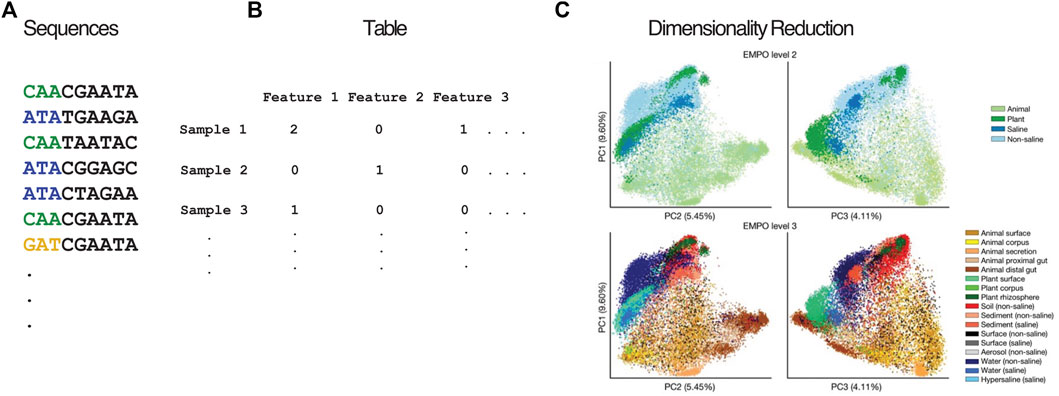
\includegraphics[width=\textwidth]{review-figures/figure01.jpeg}
\caption[Overview of dimensionality reduction pipeline.]{\textbf{Overview of dimensionality reduction pipeline.} (A)  Nucleotide sequences from a biological experiment are organized in a feature table (B) containing the abundance of each feature (e.g., OTU, ASV, MAG) in each sample. (C) Beta diversity plots showing unweighted UniFrac coordinates of EMP annotated by EMPO levels 2 and 3. (C) is a derivative of Figure 2C from “A communal catalogue reveals Earth’s multiscale microbial diversity” by Thompson et al. (2017) used under CC BY 4.0.}
\label{review_fig1}
\end{figure}

In this review, we describe how the characteristics of microbiome data complicate dimensionality reduction. We then discuss common strategies for dimensionality reduction (Table\ref{review_table1}), examining in detail whether and how they address each of the aspects that, in conjunction, confound e microbiome analysis. Tried-and-true techniques, although useful, often have conceptual and practical problems that limit their utility in the microbiome, due to the inability to handle the data's most salient traits simultaneously (Table~\ref{review_table2}). In this light, we then focus on examples of how dimensionality reduction techniques have been used in the literature, highlighting biological findings that have been revealed by each, while also discussing what may have been obscured. We then discuss common artifacts of widely used dimensionality reduction techniques, including specific pitfalls that users of these techniques must avoid in order to draw conclusions that are robust, reproducible, and well-supported by their data. We end with guidance on how dimensionality reduction should be used responsibly by practitioners in the field, and with an outlook describing how additional techniques that are seldom used today might provide valuable advances.

\begin{table}[]
\caption{Common characteristics of strategies for dimensionality reduction address different aspects of the data.}
\label{review_table1}
\centering
\begin{tabular}{p{5cm}p{9cm}}
\hline
Term & Definition \\ \hline
Compositionally   aware & Transforms data to account for   non-independence of features in sequence count data. \\
Pseudo-counts   or imputation & Requires no/minimal zeroes in   the feature table due to numerical issues (such as logarithm transform being   undefined on zeroes). \\
Able to   incorporate phylogeny & Method is calculated with   awareness of how each sampled microbial community is evolutionarily   represented relative to other samples. \\
Operates   on beta-diversity dissimilarities & Dimensionality reduction step is   performed on pairwise dissimilarities (arbitrary metric) between samples,   rather than the feature table itself. \\
Linear & Lower dimensional coordinates   are computed via linear transform of features. \\
Repeated   measures & Subjects are sampled multiple   times. Commonly sampled longitudinally. \\
Feature   relationships are interpretable & The method indicates the   relevance of input microbial features with regard to its output coordinates. \\
Supervised   component & Method takes explanatory sample   variables as an additional input.
\end{tabular}
\end{table}

\begin{sidewaystable}[]
\caption{Dimensionality reduction methods each have their own characteristics. x indicates that the characteristic applies to the method. Examples of software capable of performing each method are included in the last column. }
\label{review_table2}
\centering
\begin{tabular}{p{1.8cm}p{1.6cm}p{1.6cm}p{2cm}p{2cm}p{1.3cm}p{1.3cm}p{1.6cm}p{1.5cm}p{3.2cm}}
\hline
 & Composit-ionally aware & Avoids pseud-counts or imputation & Able to incorporate phylogeny & Operates on beta-diversity   dissimilarities & Linear & Repeat-ed Measures & Feature relationships are   interpretable & Supervised component & \multicolumn{1}{c}{Software} \\ \hline\hline
PCoA &  & x & x & x & x &  &  &  & QIIME 2, CRAN phyloseq, mothur \\\hline
PCA &  & x &  &  & x &  & x &  & scikit-learn, R built-in, mothur \\\hline
UMAP &  & x & x & x &  &  &  &  & umap-learn, CRAN umap, QIIME 2 \\\hline
t-SNE &  & x & x & x &  &  &  &  & scikit-learn, CRAN tsne \\\hline
nMDS &  & x & x & x &  &  &  &  & scikit-learn, CRAN vegan, mothur,   CRAN phyloseq \\\hline
CCA &  &  &  &  & x &  & x & x & scikit-bio, CRAN vegan, CRAN   phyloseq \\\hline
PLS-DA &  &  &  &  & x &  & x & x & CRAN mixOmics \\\hline
Aitchison   PCA & x &  &  &  & x &  & x &  & scikit-bio, QIIME 2 \\\hline
RPCA & x & x &  &  & x &  & x &  & gemelli, QIIME 2, vegan \\\hline
CTF & x & x &  &  & x & x & x &  & Gemelli, QIIME 2 \\\hline
\end{tabular}
\end{sidewaystable}

\section{Specific features of microbiome data that complicate dimensionality reduction}

“Microbiome data” most often refers to sequencing results from two primary methodologies. The first class of microbiome sequencing is known as “amplicon sequencing” where a specific gene or region of a gene is targeted in each sample. 16S, 18S, and ITS sequencing approaches all fall under this class of methods. Variants of the targeted nucleotide sequences are used as a proxy for discrete microbial taxa. These unique sequences can be clustered by sequence similarity into “operational taxonomic units” (OTUs) or used by themselves as individual units after denoisers, such as DADA2 & Deblur, resolve the individual sequence variants from error-prone sequences \cite{Callahan2017-ap,Amir2017-sk}. These filtered sequences are often called amplicon sequence variants (ASVs) \cite{Callahan2017-ap} or sub-OTUs (sOTUs). The second class of microbiome sequencing is shotgun or whole metagenome sequencing. In this method, the DNA from a sample is collected and sequenced broadly. The reads are then mapped to a reference database to determine the corresponding units, which can range from taxonomic identities to gene families or genes from a specific reference genome or metagenome-assembled genomes (MAG).

The result of these sequence analysis pipelines is typically a “feature table” that counts the microbial “units” or features (OTU, ASV, MAG, etc., [Figure~\ref{review_fig1}B]) associated with each sample. Additionally, information about the relationship between features, such as taxonomic identity or gene family, can optionally be used to “collapse” the feature table to a lower resolution sum of its units.  At this point, the data are generally ready to pursue exploratory analysis with dimensionality reduction. 
However, there are several  features common to  microbiome data that can make standard dimensionality reduction techniques difficult to apply or to interpret. Each method must therefore handle each of these key issues, or be benchmarked carefully to determine that these issues do not strongly affect the results in ways that are problematic for biological interpretation.

\subsection{High dimensionality} In this context, “dimensionality” refers to the number of features in a feature table. Microbiome data typically have far more features than samples. Across studies ranging from tens of samples to tens of thousands of samples, the number of features for taxonomic data typically exceeds the number of samples by 20-fold or more. With gene oriented data, the number of genes represented in a metagenomic study typically exceeds samples by several orders of magnitude. This can lead many statistical methods to overfit or to produce artifactual results.

\subsection{Sparsity} Most microbes are not found in most samples, even of the same biospecimen type, for example, most human stool specimens from the same population have relatively low shared taxa \cite{Allaband2019-rv}. As a result, a feature table containing counts of each microbe in each sample often has many zeros corresponding to unobserved microbes. Most 16S microbiome datasets do not have even as many as 10\% of the possible entries observed in most of the specimens. Feature tables with this over-abundance of unobserved counts are said to be “sparse”, posing problems for statistical analysis. Moreover, the proportion of observed values tends to decrease as additional samples are sequenced, often leading to tables with density well below 1\% \cite{Hamady2009-jd,McDonald2012-go}.

\subsection{Compositionality} In any high-throughput sequencing experiment, we impose an implicit limitation and randomness to the number of reads from a given sample due to many factors, including the random sub-sampling occurring both in the process of collecting samples as well as in the normalization of DNA in sequencing libraries. This limitation, termed “compositionality”, should always be kept in mind when performing any microbiome analysis on abundance data. The total number of sequences per sample can affect the distances between samples \cite{Weiss2017-iv}. Strategies such as rarefaction and relative abundance normalization are common for normalizing differences in sequencing depth. However, the relative amount of one feature in the sample is not independent from the counts of the other features–a difference in just one feature of the original sample can induce an observation that many other features are also changing \cite{Morton2019-me} and neither rarefaction or relative abundance sampling solve this issue. Due to this effect, many dimensionality reduction methods, such as principal component analysis (PCA), will emphasize false correlations in the data.

\subsection{Repeated measures} One of the most challenging experimental aspects to account for in dimensionality reduction is repeated measures data, e.g., multiple timepoints from the same subject where the variation between subjects may be greater than the variation between timepoints \cite{Wu2011-py}. In the context of dimensionality reduction, subjects or sites with multiple samples represented (such as in longitudinal studies or replicate analysis) provide an additional source of variation that can inhibit interpretation of the experimental effect of interest; the samples from a single subject can be highly correlated, resulting in between-subject differences dominating the ordination (e.g., \cite{Song2016-wt}). 

\subsection{Feature interpretation} Analysis of high-dimensional microbiome data is often motivated to find microbial biomarkers associated with observed differences in sample communities \cite{Fedarko2020-oy}. This line of inquiry is of interest for diagnosis and/or prognosis of disease status, dysbiosis, and a host of other biological questions. Although this task is often addressed with differential abundance methods, those methods make specific statistical assumptions and may not correspond to the group separation observed in an exploratory analysis performed with any dimensionality reduction method \cite{Lin2020-vq}. Thus, methods that offer a quantitative justification of their representation in terms of the microbial features are often desirable. However, methods with feature importance that are not specifically designed for the microbiome often fail to account for compositionality, which can include many false positives due to the induced correlation of features, and sparsity, where important but infrequently observed features will not be detected (false negatives).

\subsection{Complex patterns} Microbiome data are often assumed to contain clusters or gradients \cite{Kuczynski2010-gu}. For example, multiple samples swabbed from one's own keyboard are more likely to be similar to each other than samples from another individual's keyboard \cite{Fierer2010-dp}, and the microbial composition of soils is expected to vary continuously with soil pH \cite{Lauber2009-jo}. However, with larger and larger datasets with many covariates and metadata on these being collected, more complex patterns can be detected \cite{Debelius2016-ym}, such as grouping by both biological and technical factors in the case of the Human Microbiome Project \cite{The_Human_Microbiome_Project_Consortium2012-og}. Furthermore, many conventional dimensionality reduction methods, such as PCA, assume the data lie in a linear subspace, and this assumption is violated by microbiome data \cite{Potvin1993-fl,Tabachnick2013-vn,Ginter1979-ja,Greig-Smith1980-pt}.

\section{Strategies for dimensionality reduction in the microbiome}
The problems that complicate dimensionality reduction in microbiome data are scattered throughout the analysis pipeline. Difficulties can arise immediately from the raw sequence count data. Many can be corrected before the dimensionality reduction step, with careful preprocessing, though this can raise other issues. Furthemore, beta-diversity analysis, which seeks to quantify the pairwise differences in microbial communities among all samples with dissimilarity metrics (tailored to microbiome data), is often helpful for addressing many of the aforementioned circumstances \cite{Pielou1966-hn}. Algorithms that are able to incorporate these metrics are particularly valuable, and this can be done in a variety of ways. Finally, additional constraints can be placed on dimensionality reduction algorithms to account for study design or provide additional information about the correspondence between the features and the reduced dimensions. In this section, we discuss each of these strategies in depth. 

\subsection{Compositionally Aware} Comparisons between and among samples must consider how sampling and sequencing depth can affect projection into low-dimensional space. Traditionally, compositionality has been addressed using logarithmic transformations of feature ratios. Transformations such as the additive log-ratio (ALR), centered log-ratio (CLR), and isometric log-ratio (ILR) can convert  abundance data to the space of real numbers such that analysis and interpretation are less skewed by false positives \cite{Pawlowsky-Glahn2011-qk,Aitchison2002-rt}. After transformation, the Euclidean distance can be taken directly on the log-ratio transformed data (referred to as Aitchison distance)  \cite{Aitchison2002-rt}. Dimensionality reduction methods that incorporate log-ratio transformations attempt to preserve high-dimensional dissimilarities while taking into account the latent non-independence of microbial counts.

\subsection{Pseudocounts and Imputation} High-dimensional microbiome data is almost always plagued by problems of “sparsity”, or an overabundance of zeroes. The data transformations to address compositionality (as outlined above) are often based on logarithmic functions which are undefined at zero. The simplest solution is to add a small positive pseudocount to each entry of the feature table so that logarithmic functions can be applied. However, downstream analyses based on this approach are sensitive to the choice of pseudocount \cite{Kumar2018-or} and there does not exist a standardized way to choose such a value. Other options include imputation of zeros \cite{Martin-Fernandez2003-oe} through inference of the latent vector space. Fundamentally, zero handling is complicated by the inherent unknowability of the zero generating processes for each zero instance. In \cite{Silverman2020-zl}, they characterize the three different types of zero-generating processes (ZGP) as sampling, biological, and technical and demonstrate how the results of different zero-handling processes are affected by the (unknowable) mix of ZGPs in a given dataset. Recently Martino et. al. introduced a version of the CLR transform that only computes the geometric mean on the non-zero components of a given sample \cite{Martino2019-op}. This avoids the problem of logarithms being undefined at 0 and thus dimensionality reduction through this method is thus robust to the high levels of sparsity in microbiome data.

\subsection{Incorporating Phylogeny} Organisms identified using microbiome data can be related to one another through hierarchical structures that describe their evolutionary relationships. Typically, these structures take the form of either a taxonomy or a phylogeny. A taxonomy is a description of the organism relationships, generally derived subjectively using multiple biological criteria. A phylogeny, in contrast, is an inference of a tree, commonly with branch lengths, derived from quantitative algorithms that are typically applied to microbial, nucleic acid, or protein sequence data. Taxonomies have the advantage of being more directly interpretable because hierarchical structures correspond to a defined organization and classification pattern curated by experts in the field. However, these assignments and hierarchies are often putative and subject to change as more information about microbial taxa emerges. In contrast, phylogenies are derived from quantitative measures of sequence similarity from sample reads. These data structures are more easily incorporated into statistical analyses but often at the cost of less interpretability as the hierarchical structures do not necessarily map to pre-defined microbial relationships. These evolutionary relationships, particularly phylogenies, add information to microbiome analysis, because related organisms are more likely to exhibit similar phenotypes (although counterexamples do exist, especially closely related taxa such as \textit{Escherichia} and \textit{Shigella}, which are very similar genetically but produce different clinical phenotypes).

When comparing the similarity of pairs of microbial communities, it is possible to utilize these hierarchical structures, and derive a metric that computes a distance as a function of shared evolutionary history \cite{Lozupone2005-aj}. Specifically, communities that are very similar will share most of their evolutionary history, whereas those that are very dissimilar will have relatively little in common. A popular form of phylogenetically-aware distances is the suite of UniFrac metrics, which includes both quantitative \cite{Lozupone2007-gw} and qualitative \cite{Lozupone2005-aj} forms. Numerous extensions to UniFrac have been developed \cite{Chen2012-ti,Chang2011-gt}, including variants that account explicitly for the compositional nature of microbiome data \cite{Wong2016-sx}. Because these metrics all utilize not only exactly observed features, but also the relationships among features, they can better account for the sparsity of microbiome data which manifests at the tips of a phylogenetic tree (because most microbes are not observed in most environments). In contrast, a metric like the Euclidean distance is limited to only the information at the tips of these hierarchies, and, worse, assumes that all features at the tips are equally related to one another (so that in a tree consisting of a mouse, a rat, and a squid, there is no allowance for the fact that the two rodents are much more similar to each other than they are to the squid). Neither phylogenetic nor non-phylogenetic beta-diversity measures explicitly model differences in sequencing depth per sample (this occurs because of uncontrolled variation in how efficiently each sample is amplified and incorporated into molecular libraries for sequencing), although these differences in depth can be standardized through rarefaction \cite{Weiss2017-iv}. 

\subsection{Operates on Generalized Beta-Diversity Matrix} Many of the issues outlined above can be easily addressed at the sample dissimilarity level rather than directly through dimensionality reduction algorithms. A number of dissimilarity/distance metrics have been developed to account for factors such as phylogenetic data incorporation, compositionality, or sparsity that output a sample by sample matrix estimating high-dimensional dissimilarity. These dissimilarity matrices represent the overall community differences between pairwise samples calculated by a chosen beta-diversity metric. Dimensionality reduction methods that operate on arbitrary dissimilarity metrics are attractive options because the complex handling of the various feature table issues can be split into the choice of dissimilarity metric and the choice of dimensionality reduction algorithm. This adds a layer of flexibility for researchers to analyze their data depending on their needs. Methods based on multidimensional scaling approaches such as PCoA \cite{Kruskal1978-xx} and nMDS \cite{Kruskal1964-dn}attempt to preserve as much as possible the pairwise distances between subjects. Other methods such as t-distributed stochastic neighbor embedding (t-SNE) \cite{Van_der_Maaten2008-af} and Uniform Manifold Approximation and Projection (UMAP) \cite{McInnes2018-zd} are non-linear dimensionality reduction techniques that aim to find a low-dimensional representation such that similar data points are placed closed together and dissimilar points are pushed apart. A caveat of these methods is that they can be very sensitive to the choice of dissimilarity used. Patterns that may appear from one measure of dissimilarity may not be as apparent in a different measure. As an example, phylogenetic metrics such as UniFrac may differ from non-phylogenetic metrics such as Bray-Curtis depending on the strength of phylogenetic contribution \cite{Shankar2017-af}. The choice of dissimilarity metric should therefore be considered carefully, as different dimensionality reduction techniques yield visually and statistically very different results on the same data \cite{Kuczynski2011-yx}.

\subsection{Linear vs. Non-Linear Methods} Principal coordinates analysis (PCoA) and PCA are popular dimensionality reduction techniques that fall under the ``linear" category. Linear techniques attempt to reduce or transform the data such that an approximation of the original data can be reconstructed by a weighted sum of the resulting coordinates. These methods typically involve computing decompositions/factorizations of the data that are highly computationally efficient and work well on data that is naturally linear. Various other techniques, such as robust Aitchison PCA (RPCA) \cite{Martino2019-op}, and nonnegative matrix factorization (NMF) \cite{Lee1999-bu} also fall under this class of techniques.

Other methods fall under the ``non-linear" category, which perform more complex transformations that often excel at preserving different patterns that may not be linear. This category includes methods such as the non-metric multidimensional scaling (nMDS), t-SNE, and UMAP. These methods can more succinctly represent complex patterns, but possibly at the expense of additional computation. Furthermore, these models tend to have randomness (such as from initialization) and more hyperparameters that the output can be highly sensitive to, so it is usually necessary to run these algorithms multiple times to ensure the conclusions are reproducible. Other non-linear methods that have seen less frequent use in the microbiome data (and bioinformatics generally) include kernel PCA \cite{Scholkopf1999-nw}, locally linear embeddings \cite{Roweis2000-jp}, Laplacian eigenmaps \cite{Belkin2001-ip}, and ISOMAP \cite{Tenenbaum2000-dy}.

Unlike its close, linear counterpart PCoA, nMDS performs the ordination onto a pre-specified number of dimensions and operates on the ranks of the dissimilarities, rather than the dissimilarities themselves. This rank-based approach can be beneficial for representing data that departs from the assumptions of linearity. Other non-linear methods, such as t-SNE and UMAP, also transform the data onto a pre-specified number of dimensions, and operate by assuming the high-dimensional data follows a non-linear structure that can be represented with fewer dimensions. 

\subsection{Repeated Measures} If the biological variable of interest occurs at the subject level, repeated samples (such as through a longitudinal study design) can artificially inflate how tight a cluster appears in low-dimensional space. Dimensionality reduction methods for microbiome need to be designed for the purpose of handling this kind of data, with the intent to represent the relationships between explanatory variables while accounting for the inherent similarity between samples from the same subject. Methods to account for repeated measures can incorporate the relationship between individual samples and subjects by machine learning approaches \cite{Martino2021-wa}. There has also been discussion about incorporating prior sample relationship information into ordinations through Bayesian methods \cite{Ren2017-pu}. Nevertheless, methods that incorporate repeated measures remain an underexplored area in dimensionality reduction literature.

\subsection{Feature Importance} When the lower-dimensional representation of microbial communities shows separation between sample groups, a natural next question is what microbes or groups of microbes are driving such a separation. Dimensionality reduction methods that return a quantitative relationship between individual microbial features and the latent lower-dimensional space are a powerful class of methods that can demystify the construction of the lower-dimensional axes. However, certain methods that attempt to find high-dimensional patterns, such as non-linear methods, do not have an explicit interpretable correspondence between the output coordinates and the input features.

The most relevant category of methods that do provide feature importance is the biplot ordination family of approaches. Biplots display both the samples and the driving variable vectors in reduced dimension space (Figure~\ref{review_fig2} A,D,E,H). For example, PCA naturally quantifies the contribution of each microbe to the principal component axes through matrix factorization into linear combinations of features. RPCA modifies this approach to account for compositionality and sparsity while retaining interpretable feature loadings \cite{Martino2019-op}. Another set of ecologically motivated matrix factorization methods is the correspondence analysis (CA) family. The general CA method can be thought of as an implementation of PCA that operates on count data. It is also possible to explicitly incorporate sample metadata into these dimensionality reduction methods. Researchers are often interested in the explanatory power of their sample metadata (site, pH, subject, etc.). Certain dimensionality reduction methods can take as input both a feature table and a table of sample metadata to jointly estimate the low-dimensional representation of samples as well as the relative contribution of the provided metadata vectors. The general goal of these methods is to determine whether and/or which explanatory variables may be driving the differences in microbial communities among samples. Canonical correspondence analysis (CCA) is an extension of CA that incorporates sample variables of interest to determine which covariates are associated with the placement of samples and feature vectors in low-dimensional space \cite{Ter_Braak1985-ge}. The results of CCA can be visualized as a “tri-plot” where samples are simultaneously visualized with the relative contribution of features and explanatory variables near related samples. \cite{Ruiz-Perez2020-tb,Paliy2016-az} Partial least squares discriminant analysis (PLS-DA) is a similar approach that uses only categorical sample metadata (classification) in the construction of lower-dimensional axes \cite{Barker2003-ce,Ruiz-Perez2020-tb}. The contribution of these sample variables can then be quantified and visualized in the projection, motivating subsequent statistical analysis of associations between sample metadata and specific microbial taxa.

\begin{figure}[htbp]
\centering
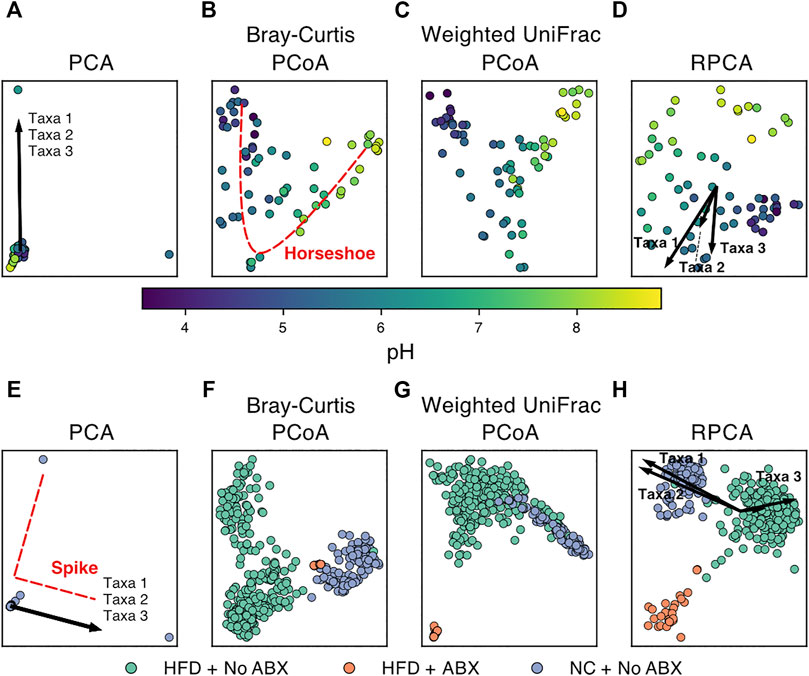
\includegraphics[width=\textwidth]{review-figures/figure02.jpeg}
\caption[Examples of dimensionality reduction techniques applied to publicly available microbiome data]{\textbf{Examples of dimensionality reduction techniques applied to publicly available microbiome data.} (Top) Beta-diversity plots of soil samples colored by pH from \cite{Lauber2009-jo}. (Bottom) Beta-diversity plots of murine fecal samples colored by diet and antibiotics usage from \cite{Shalapour2017-iv}. (HFD = high-fat diet, NC = normal chow, ABX = antibiotics). PCA plots (A,E) show extremely high sample overlap due to outliers and characteristic “spike” artifacts. The top three taxa driving variation also overlap as shown by arrow superposition. (B) “Horseshoe” pattern emerges for samples following ecological gradients such as pH. RPCA plots (D,H) show the top three taxa driving separation of groups. (F) and (G) show strong overlap of HFD + ABX samples resolved by (H).}
\label{review_fig2}
\end{figure}

\section{Uses of dimensionality reduction for microbiome data}

Over the past decade, PCoA has seen an increase in use in microbiome analyses, and it is the primary ordination method for beta-diversity included by default in workflows such as QIIME2 \cite{Bolyen2019-fq}. It is typically used for exploratory visualization, as it excels at rendering biologically relevant patterns, such as clusters and gradients \cite{Kuczynski2010-gu}. When used as an exploratory tool, observed patterns are often followed with statistical analysis on the original feature tables or dissimilarity matrices \cite{Galloway-Pena2020-fg}, such as ANOSIM \cite{Clarke1993-ad}, PERMANOVA (aka Adonis) \cite{Anderson2017-og}, ANCOM \cite{Mandal2015-pm}, or bioenv \cite{Clarke1993-ad}. It should also be noted that some of these statistical techniques use the full table or dissimilarity matrix, not the reduced dimension matrix as visualized (at least by default), and may therefore introduce incongruent results between the statistics and the visualization.

Exploratory visualizations have revealed microbial-associated patterns in applications ranging from host-associated gut microbiomes to soil, ocean, and other environmental microbiome contexts. For example, studies have applied PCoA to demonstrate differences between host groups, such as differences between humans', chimpanzees', and gorillas' gut microbial taxa \cite{Campbell2020-hj}, or the correspondence between human gut microbiomes and westernization \cite{Campbell2020-hj,Yatsunenko2012-wv}. Host microbiome-disease associations have also been identified using PCoA, such as in the case of colorectal cancer \cite{Young2021-ho} in humans and metritis in cows \cite{noauthor_2019-us}. Uses also extend to host-environment relationships, such as demonstrating the differences between oyster digestive glands, oyster shells, and their surrounding soils \cite{Arfken2017-hy}. The microbiome-shaping roles of environmental factors such as salinity in shaping free-living environments \cite{Lozupone2007-yr}, pH in arctic soils \cite{Malard2019-rk} and depth in the ocean \cite{Sunagawa2015-gg} have also been elucidated with PCoA. In many of these cases, the PCoA visualizations demonstrating separation between groups were subsequently followed by statistical validation with PERMANOVA or ANOSIM.

In numerous other instances, PCoA has also been used to make claims that extend beyond exploratory group differences followed by statistical analysis. For example, Halfvarson et al. fit a plane to the healthy subjects in the first three coordinates of a PCoA and then used the distance to this plane to associate dissimilarities in the microbiome with the severity of irritable bowel disease (IBD) \cite{Halfvarson2017-se}; this approach has subsequently been replicated \cite{Gonzalez2018-ez}. Others have used regression of participant and microbiome characteristics (e.g., age and alpha diversity, respectively) on PCoA coordinates to determine whether the given factors have a significant relationship with microbial community composition in the context of dietary interventions \cite{Lang2018-io}. In one case, while providing visualization with PCoA and statistical confirmation with ANOSIM, Vangay et al. additionally plotted ellipses for visualizing cluster centers/spread in their PCoA coordinates \cite{Vangay2018-qf}. In another instance, Metcalf et al. showed the correspondence of dissimilarities between the 16S rRNA profiles and chloroplast marker profiles by performing a Procrustes analysis on the separate ordinations of the different data types \cite{Metcalf2017-me}.

We note that the choice of dissimilarity metric can have a significant impact on the low-rank embedding depending on the dataset. Shi et. al. review the effect of high and low-abundance operational taxonomic units have on unsupervised clustering of Bray-Curtis and unweighted UniFrac \cite{Shi2021-ln}. Marshall et. al compare Bray-Curtis ordination with weighted UniFrac on marine sediment samples and note that the most relevant clustering variable differed depending on the dissimilarity used \cite{Marshall2019-nc}. These results imply that interpretation of low-dimensional embeddings and the putative driving variables must be performed in the context of the choice of dissimilarity. Metrics such as Bray-Curtis and weighted UniFrac take into consideration the abundance of individual microbes in each sample which can be important for datasets with many rare taxa. In contrast, some dissimilarity metrics such as Jaccard and unweighted UniFrac are only defined on presence-absence data, which may mask this property.  Furthermore, phylogenetic metrics such as the UniFrac suite of metrics are best when the evolutionary relationships among microbial features is of interest in the context of sample communities. These metrics may also be more appropriate than other methods for datasets with particularly high sparsity.

PCA is arguably the most widely used and popular form of dimensionality reduction, which does not allow generalized beta-diversity distances (e.g., PCoA or UMAP), but does allow for the direct interpretation of feature importances relative to sample separations in the ordination. However, due to compositionality and sparsity, PCA often leads to spurious results on microbiome data \cite{Morton2017-bs,Hamady2009-jd}. Aitchison PCA attempts to fix these issues by using log transformation, but imputation is required (because the log of zero is undefined). Therefore, \cite{Martino2019-op} proposed the adoption of RPCA for dimensionality reduction. This method has been shown to discriminate between sample groups in a wide array of biological contexts, including fecal microbiota transplants \cite{Goloshchapov2019-pe}, cancer \cite{Bali2021-nw}, and HIV \cite{Parbie2021-mm}. Moreover, the generalized version of this technique accounts for repeated measures, allowing for large improvements in the ability to discriminate subjects by phenotypes across time or space \cite{Martino2021-wa}. This advantage has been crucial in the statistical analysis of complicated longitudinal experimental designs such as early infant development models \cite{Song2021-bi}. Feature loadings from these PCA-based methods can be used to inform selection of microbial features for log-ratio analysis \cite{Fedarko2020-oy,Morton2019-me}, leading to novel biomarker discovery.

For feature interpretation, CCA is the most commonly used CA-based method for analyzing high dimensional microbiome data, due to its ability to incorporate sample metadata into the low-rank embeddings. This strategy has shown success in differentiating clinical outcomes following stem cell transplantation \cite{Ingham2019-ei} as well as diarrhea status in children \cite{Dinleyici2018-ka}. CCA has also shown success in projecting environmental samples into lower-dimensional space such as in rhizosphere microbial communities \cite{Benitez2017-xy,Perez-Jaramillo2017-vt}, and aerosol samples \cite{Souza2021-ce}. Another approach designed for microbial feature interpretation has been posed by \cite{Xu2021-uk}, explicitly modeling the ZGP through a zero-inflation model. This method attempts to optimize a statistical model for jointly estimating the “true” zero-generating probability as well as the Poisson rate of each microbial count.

Of non-linear methods, nMDS has historically been more widely used in microbiome data analysis, in part because it can incorporate an arbitrary dissimilarity measure. Furthermore, since nMDS is a rank-based approach, it is less likely than linear methods to be highly influenced by outliers in beta-diversity dissimilarities. Recent uses have involved using nMDS to show differences in the gastric microbiome between samples from patients with gastric cancer cases against the control of gastric dyspepsia (recurrent indigestion without apparent cause) \cite{Castano-Rodriguez2017-ns} and demonstrating differences in the gut microbiome based on diabetes status \cite{Das2021-dw}. In both of these cases, the visual distinction between groups was supported by PERMANOVA.

Other non-linear methods have been increasingly used for analyzing other types of sequencing data, especially in the single-cell genomics field, but have not yet been widely deployed in the microbiome. The most popular of these methods for visualization, t-SNE and UMAP, are starting to see more use in the microbiome field. \cite{Xu2020-ht} developed a method to classify microbiome samples using t-SNE embeddings. We recently reviewed the usage and provided recommendations for implementing UMAP for microbiome data \cite{Armstrong2021-tr}. UMAP with an input beta-diversity dissimilarity matrix can reveal biological signals that may be difficult to see with traditional methods such as PCoA. 

\section{Artifacts and cautionary tales in dimensionality reduction}

Dimensionality reduction is incredibly useful and has led to many interesting biological conclusions. However, when using dimensionality reduction techniques, one must be careful how results are interpreted. There are known examples of patterns that are induced by the properties of the data alone (rather than the relationships among specific samples or groups of samples), and others that are a product of the method itself. Here, we discuss several known issues, as well as insights to evaluating the degree to which an ordination represents the actual data.

One of the most well-known artifacts in microbial ecology is the horseshoe effect \cite{Podani2002-vg}, wherein the ordination has a curvilinear pattern along what otherwise appears to be a linear gradient. This pattern can occur when a variable, such as soil pH \cite{Lauber2009-jo} or length of time of corpse decay \cite{Metcalf2016-iq} corresponds with drastic changes in microbiome composition on a continuous scale. Since the characteristic ``bend'' in the horseshoe typically occurs along the second coordinate of a PCoA (Figure~\ref{review_fig2}), it can obfuscate additional gradients/associations along that axis. Recent research in the topic has also identified that indeed, it is unlikely the horseshoe appears from a real effect, and instead it is a product of the limitations of many distance metrics to capture distance along a gradient when no features are shared between many of the samples (i.e., saturation) \cite{Morton2017-bs}, which can be an issue with many common metrics, such as Euclidean, Jaccard, and Bray-Curtis distances\cite{Morton2017-bs}. As a result, a possible remedy for the artifact is to use a distance metric  that considers the relationships between features, such that two samples that share no features do not necessarily have the same dissimilarity as two different samples that share no features, e.g., UniFrac or weighted UniFrac. If a phylogenetic metric does not resolve the issue, it may be possible to avoid the horseshoe artifact by using RPCA or a non-linear method (e.g., UMAP).  "Spikes" are another artifact, more prevalent on cluster-structured data, where outliers dominate the embedding and it fails to separate into clusters in the visualization \cite{Vazquez-Baeza2017-yp}. Spikes also appear to be mitigated with an appropriate choice in distance metric, such as UniFrac \cite{Hamady2009-jd}. In both cases, since the issues are with representing the distances between distant or extreme samples, non-linear methods (such as UMAP or nMDS) that disregard the distance values of outliers to provide a potential workaround to reveal secondary gradients or the obfuscated cluster structures \cite{Armstrong2021-tr}. Though it is possible that the benefits offered by non-linear methods for the horseshoe effect are limited by the aspect ratio of the gradient \cite{Kohli2021-fk}, and potentially the parameters of the algorithms.

Dimensionality reduction is also commonly used in other bioinformatic disciplines. Particularly, single-cell transcriptomics has used dimensionality reduction prolifically, with many publications using PCA, t-SNE, or UMAP visualizations. Furthermore, single-cell RNA-seq data shares many properties with microbiome data, including sparsity/zero-inflation, sequencing depth differences, and even phylogenetic relationships \cite{Lahnemann2020-ky}. This connection is further strengthened by the fact that researchers in both disciplines investigate similar types of questions, albeit with different underlying data. Microbiome researchers often ask whether there is a difference between different treatments or disease-statuses \cite{Llorens-Rico2021-dr,David2013-ps}, and which microbes contribute to those differences (i.e., differential abundance analysis). Similarly, transcriptomics may investigate parallel scenarios \cite{Ocasio2019-lb,Taavitsainen2021-ib}, where the goal is to discover transcripts whose expression stratifies the desired groups (i.e., differential expression).

Despite these similarities, the most popular methods for dimensionality reduction in microbiome and single-cell publications differ significantly, with PCoA being more prevalent among microbiome publications, and t-SNE (or variants \cite{Linderman2019-mt}) and UMAP more prevalent in single-cell publications \cite{Kobak2019-gk}. Given the similarities in hypotheses and the properties of the data, but use of different methods, it is reasonable to suppose that methods such as t-SNE and UMAP have potential utility in the microbiome. However, global distances are not necessarily preserved in these methods, therefore distances between different clusters should not be interpreted as demonstrating similarity or dissimilarity. Consequently, recent research concerning the representation of single-cell RNA-seq research should also be taken into account when applying these methods to microbiome data.

First, t-SNE and UMAP are fairly complex algorithms that have many hyperparameters that can be adjusted, so it is important to be able to evaluate the faithfulness of the embeddings they produce. The evaluation of dimensionality reduction has been performed with many different measures, each of which has its own characteristics. Some measures reward embeddings that adequately preserve the local-scale structures in the embedding but do not necessarily penalize inaccurate representations of large distances in the original high-dimensional data, like the KNN evaluation measure \cite{Kobak2019-gk}, which takes the average accuracy of the k=10 nearest neighbors in the reduced dimensions compared to the original space. Others, such as the correlation (either Pearson or Spearman) between distances in the original space and reduced dimensions have been used \cite{Kobak2019-gk,Kobak2021-ih,Becht2019-hm}. The correlation measure generalizes whether the two representations overall are similar, i.e. close points in the original space are close in the low-dimensional space, and similar for far points. However, high correlation does not guarantee that the fine-scale structures have been preserved. Additionally, measures that use additional metadata about known classes can be used, such as the KNC measure \cite{Kobak2019-gk}, which measures whether the closest class/category centers to a given center are preserved in the embedding. KNC emphasizes the preservation of relationships between classes, but not necessarily structures within the classes or between distant classes. These measures have been used to evaluate the quality of several dimensionality reduction methods across a variety of parameter settings on complex datasets. Notably, Kobak and Berens (2019) demonstrated on several single-cell transcriptomics datasets, that t-SNE with the default value for ``perplexity" performed well at representing the relationships between nearby points (KNN), but poorly at representing the large-scale patterns (KNC and CPD). However, when they increased the perplexity parameter, they achieved improved KNC and CPD at the expense of a decreased KNN score \cite{Kobak2019-gk}. Kobak and Linderman (2021) observed with CPD that the best method (between t-SNE and UMAP) can vary by dataset \cite{Kobak2021-ih}. So, in practice, it may be necessary to compare multiple dimensionality reduction methods (and parameter settings) on a dataset using the measure that best suits the question, e.g., use the CPD measure when seeking a visualization of earth microbiomes by environment to show which environments are similar to each other.

Furthermore, since UMAP and t-SNE are algorithms that require configurable (possibly random) initializations, particular attention has been paid to their reproducibility. A metric to evaluate reproducibility comes from \cite{Becht2019-hm}, which measures the preservation of pairwise distances in the embeddings by comparing an embedding on a subset of the points to location of those points in the embedding of the entire dataset. In its original application, the reproducibility measure was used to demonstrate UMAP providing more reproducible results than t-SNE and variants of t-SNE. However, \cite{Kobak2021-ih} showed that with appropriate (spectral) initialization, t-SNE can perform just as well by this metric as UMAP. While reproducibility is important, this metric should be applied carefully, because it fails to account for rotations in the embedding. Another important concern related to reproducibility is whether even random noise will yield apparent clusters. This phenomenon has been observed with t-SNE \cite{Wattenberg2016-oh}, and whether other dimensionality reduction techniques are also susceptible to this effect warrants further systematic investigation. However, because these benchmarks are all performed within transcriptomics, further validation is needed to determine whether the conclusions generalize to microbiome data.  These measures provide a starting point for evaluating the application of non-linear dimensionality reduction techniques on microbiome data.

Finally, literature from mathematics and computer science that has not been as widely applied to dimensionality reduction in bioinformatics may also be relevant. Of particular interest is the study of distortion, which is applicable when the goal of the embedding is to preserve distances, like one might expect for an exploratory analysis. Similar to the previously described correlation measure, distortion measures summarize the extent to which the distances in high dimensions match the distances in low-dimensions, however, distortion is defined in terms of the expansions and contractions of distances between points. Furthermore, there are many ways to summarize the expansions and contractions, including the worst-case, average-case and local-case, which are all detailed more in \cite{Vankadara2018-sm}. 

\section{Discussion}

The above examples illustrate that dimensionality reduction is an extremely powerful technique that has enhanced a wide range of microbiome studies. However, with great power comes great responsibility. It is unlikely that any one method will excel at representing all datasets, so responsible users of dimensionality reduction should try out several techniques, ideally guided by characteristics of the data rather than as a fishing expedition to see whether any one of many techniques produce results that “look good” (which may even happen in random data for some techniques and parameters) or that fulfill pre-conceived hypotheses and biases. We need standard protocols and software interfaces for choosing the algorithm that suits your data best, rather than the algorithm that shows what you want to see if you squint at it correctly. Methods are needed both for diagnosing the issues that may be most prevalent in your data and affecting your representation, and for rationally choosing among different methods that could be applied to a given dataset. Developing these methods is a key priority for the field.

Dimensionality reduction for the purposes of visualization has somewhat different goals from dimensionality reduction for other purposes, and developing a better appreciation of this distinction is important for practice in the field. The goal of dimensionality reduction for visualization is primarily for exploratory overview by human observers (do groups differ from one another, is there overall structure such as gradients in the data). As such, visualization is usually done with three dimensions (more can be examined through parallel plots), while the intrinsic dimensionality of the data may be higher. Visualization is typically only the first step in the data analysis pipeline, and is followed by downstream analysis, such as multivariate analysis/regression (PERMANOVA, ANOSIM, PERMDISP) either on the original distances or on a dimensionality-reduced version of the data (which can be higher than three dimensions). These results can also be used to motivate supervised differential abundance modeling, such as to determine which groups separate and then determine which microbes are driving these separations.

Dimensionality reduction is thus often an early step in a multi-step pipeline. What downstream analyses is dimensionality reduction a step towards, and how are these accomplished? Feature loadings (i.e., the importance of particular taxa or genes) can be interpreted using log ratios in tools such as DEICODE, which can then be visualized in Qurro. Classification can be accomplished using machine learning techniques such as random forests, allowing estimates of classifier accuracy and group stability, and also allowing tests of the reusability of these models, e.g., applying a model of human inflammatory bowel disease to dogs \cite{Vazquez-Baeza2016-sq} or models of aging between different human populations \cite{Huang2020-iw}. A popular strategy is to use a lower-dimensional embedding for traditional statistical analysis, such as using PCA or PCoA coordinates as inputs for regression, classification, clustering, and other analyses. However, as we have seen, many dimensionality reduction methods induce various kinds of artifacts or distortions, and cannot generalize well beyond the data on which the model was initially optimized on, including, PCoA, nMDS, RPCA/CTF, and UMAP/t-SNE. Consequently, analyses on these coordinates should be performed with caution. Furthermore, since the parameters and software versions used with these methods have the potential to be highly influential to their results, we recommend that these always be reported for dimensionality reduction methods.

Given the large numbers of publications that have used dimensionality reduction on microbiome data, we can start to draw conclusions about which dimensionality reduction strategies should be more widely used, and which less widely used. On larger, sparser, compositional datasets, we recommend against the use of conventional PCA, Bray-Curtis and Jaccard distances, and pseudocounts. Conventional PCA presents the clearest case of a method that should not be used on microbiome data due the sparsity and compositional nature of the data. UniFrac and weighted UniFrac are essentially phylogenetically informed versions of Jaccard and Bray-Curtis beta-diversity metrics respectively. Due to the current default generation of a phylogeny in most 16S and shotgun analyses, there is no reason not to use the phylogenetic counterparts, which have been shown to have better discriminatory power. Pseudocounts should not be used because the choice of pseudocount impacts the lower-dimensional embedding, and there is no clear method for determining which pseudocount value is best.

In contrast, CTF and non-linear methods should be used more in microbiome contexts. As the cost of acquiring microbiome data continues to decrease, experimental designs are getting increasingly complex, and include repeated measures, longitudinal studies, batch effects, etc. We therefore need methods that can determine which biological signals are relevant among all these confounding factors. Additionally, we are increasingly recognizing that many relationships between/among samples are non-linear. Using non-linear methods can potentially explain more of such datasets with fewer dimensions, although additional benchmarking is required to understand the performance of these methods. 

Our analyses suggest some important gaps in the field that could be important areas for future development. There are no dimensionality reduction methods yet that are both able to incorporate phylogeny and are compositionally aware. Several methods, such as Robust PCA and CTF, control for the sparsity, non-normality, compositionality, and are adaptable to specific study-designs of microbiome data but do not incorporate phylogenetic information. In contrast, phylogenetic techniques do not account for sparsity and compositionality, and some also perform poorly with non-normality. A unified method that is appropriate for any microbiome study is therefore still in the future, despite many important recent advances. The ability to perform this task using a generalizable dissimilarity measure would be particularly useful, because it would allow for full utilization of PCoA and non-linear methods including nMDS and UMAP.

Taken together, we conclude that dimensionality reduction is a key part of many, if not most, of the highest-impact microbiome studies performed to date. We can expect this situation to continue into the future, especially as larger study designs and datasets continue to accumulate, and additional method development advances increase the speed and range of applicability of these techniques.






\section{Acknowledgments}

This work was supported in part by grants NSF 2038509, NIH U24CA248454, NIH 1DP1AT010885, and by CRISP, one of six centers in JUMP, a Semiconductor Research Corporation (SRC) program sponsored by DARPA.

Chapter~\ref{chapter_review}, in full, is a reprint of the material as it appears in ``Applications and Comparison of Dimensionality Reduction Methods for Microbiome Data.'' George Armstrong, Gibraan Rahman, Cameron Martino, Daniel McDonald, Antonio Gonzalez, Gal Mishne, and Rob Knight. \textit{Frontiers in Bioinformatics 2}, 2022. The dissertation author was the primary investigator and co-first author of this paper.







\chapter{Efficient computation of Faith’s phylogenetic diversity with applications in characterizing microbiomes}\label{chapter_faiths_pd}


\glsresetall

% \section{Abstract}
The number of publicly available microbiome samples is continually growing. As dataset size increases, bottlenecks arise in standard analytical pipelines. Faith’s phylogenetic diversity is a highly utilized phylogenetic alpha diversity metric that has thus far failed to effectively scale to trees with millions of vertices. Stacked Faith's Phylogenetic Diversity (SFPhD) enables calculation of this widely adopted diversity metric at a much larger scale by implementing a computationally efficient algorithm.  The algorithm reduces the amount of computational resources required, resulting in more accessible software with a reduced carbon footprint, as compared to previous approaches. The new algorithm produces identical results to the previous method. We further demonstrate that the phylogenetic aspect of Faith's PD provides increased power in detecting diversity differences between younger and older populations in the FINRISK study's metagenomic data.

\section{Introduction}

In microbiome research, particular attention is given to evaluating the diversity of microbes within samples \cite{McDonald2018-uf,The_Human_Microbiome_Project_Consortium2012-og,Thompson2017-pu}.  Alpha diversity (within sample diversity), in particular, can summarize the breadth of microbial diversity present in a sample. There are many examples of associations between various host factors and alpha diversity, including country \cite{McDonald2018-uf}, disease status \cite{Gevers2014-bs,Vazquez-Baeza2016-sq}, diet \cite{McDonald2018-uf}, and age \cite{Yatsunenko2012-wv} among many others \cite{Youngblut2019-pk,Jeffery2016-rc}.
Modern DNA sequencing instruments have enabled microbiome studies at the scale of tens of thousands of samples, which presents a computational challenge for metrics that rely on a phylogeny, such as Faith’s Phylogenetic Diversity (Faith’s PD) \cite{Faith1992-gh}. Faith’s PD is computed by summing the branch lengths (edge weights) of the phylogeny that exclusively represent the sequences contained in a biological sample. The amount of memory and number of necessary operations needed to calculate Faith's PD depends on the number of edges in the phylogenetic tree, as well as the number of samples in the underlying data table.
In today’s increasingly large and sparse datasets and meta-analyses, these phylogenetic trees and tables can exceed 100,000s of samples and millions of tree tips \cite{McDonald2018-qq}. Recent advances have enabled efficient computation of the UniFrac metric for beta diversity, which is also a metric computed over phylogenetic trees \cite{Lozupone2005-aj}. Specifically, Striped UniFrac \cite{McDonald2018-qq} improves upon previous UniFrac implementations \cite{Hamady2010-dg} by using space- and time-efficient tree data structures \cite{Cordova2016-vf} and reducing the number of vectors required to store intermediate scores in the tree. 
Additionally, the usefulness of techniques like Faith’s PD and UniFrac remains underexplored for metagenomics sequencing. Recent molecular protocol optimizations, such as SHOGUN \cite{Hillmann2018-vk}, have enabled the metagenomic characterization of large human cohorts  \cite{Salosensaari2020-tx,Borodulin2015-uz,Kaplan2019-yo}. In this context, the applicability of Faith’s PD has largely been limited by the technical difficulties associated with constructing phylogenies from metagenomic features \cite{Zhu2019-od}. Efforts like the Web of LIfe (WoL) \cite{Zhu2019-od} and Genome Taxonomy Database (GTDB) \cite{Parks2020-cg,Parks2018-gb} are now addressing this issue by providing a phylogenomic tree as part of their database releases that can be used for phylogeny-informed analysis.

Motivated by these advances in algorithms and resources for analyzing phylogenies, phylogenomic trees, and sparse data, we developed a new algorithm and implementation, Stacked Faith's Phylogenetic Diversity (SFPhD), for rapidly computing Faith’s PD. SFPhD produces identical results to those of previous algorithms for computing this metric while producing a speedup of up to 64x and requiring as little as 0.21\% of the memory in our benchmarks (Table~\ref{faiths_pd_table1}). The key advances of SFPhD are using a sparse matrix representation, an efficient tree structure, and partial aggregation of metric constituents. Our BSD-licensed implementation of this algorithm is available in the `unifrac' package (via PyPI and bioconda \cite{Gruning2018-fw}), which has 50,714 total conda downloads and 34,141 conda downloads since the introduction of SFPhD, as of the time of writing (May 13, 2021). The package produces a C/C++ shared library with Python bindings and is additionally linkable by any programming language (https://github.com/biocore/unifrac). Additionally, by investigating the previously documented relationship between age and bacterial richness of the gut microbiome \cite{De_la_Cuesta-Zuluaga2019-zr}, we demonstrate that accounting for phylogeny in metagenomic data can increase the statistical power for detecting group differences. 

% \usepackage{colortbl}

\begin{sidewaystable}
\caption[Average memory improvement and speedup of SFPhD compared to the reference implementation.]{Average memory improvement and speedup of SFPhD compared to the reference implementation.}
\label{faiths_pd_table1}
\centering
\begin{tabular}{|c|rrr|rrr|}
\hline
\multicolumn{1}{|l|}{} & \multicolumn{3}{l|}{Time (s)}                                                                                         & \multicolumn{3}{l|}{Memory (kbytes)}                                                                                      \\ \hline
\textbf{\# of Samples} & \multicolumn{1}{c|}{\textbf{skbio}} & \multicolumn{1}{c|}{\textbf{SFPhD}} & \multicolumn{1}{c|}{\textbf{Speedup (x)}} & \multicolumn{1}{c|}{\textbf{skbio}} & \multicolumn{1}{c|}{\textbf{SFPhD}} & \multicolumn{1}{c|}{\textbf{Improvement (x)}} \\ \hline
\textbf{1250}          & \multicolumn{1}{r|}{18.6}           & \multicolumn{1}{r|}{4.67}           & 3.98                                      & \multicolumn{1}{r|}{10001242.8}     & \multicolumn{1}{r|}{312815.6}       & 31.97                                         \\ \hline
\textbf{2500}          & \multicolumn{1}{r|}{32.8}           & \multicolumn{1}{r|}{5.12}           & 6.41                                      & \multicolumn{1}{r|}{19114300.4}     & \multicolumn{1}{r|}{313834.8}       & 60.91                                         \\ \hline
\textbf{5000}          & \multicolumn{1}{r|}{79.75}          & \multicolumn{1}{r|}{6.31}           & 12.64                                     & \multicolumn{1}{r|}{36727706.4}     & \multicolumn{1}{r|}{315124}         & 116.55                                        \\ \hline
\textbf{10000}         & \multicolumn{1}{r|}{270.34}         & \multicolumn{1}{r|}{8.76}           & 30.86                                     & \multicolumn{1}{r|}{75866321.6}     & \multicolumn{1}{r|}{317413.2}       & 239.01                                        \\ \hline
\textbf{20000}         & \multicolumn{1}{r|}{910.62}         & \multicolumn{1}{r|}{14.17}          & 64.26                                     & \multicolumn{1}{r|}{152783905.2}    & \multicolumn{1}{r|}{320837.6}       & 476.2                                         \\ \hline
\textbf{40000}         & \multicolumn{1}{l|}{*}              & \multicolumn{1}{r|}{25.58}          & \multicolumn{1}{l|}{N/A}                  & \multicolumn{1}{l|}{*}              & \multicolumn{1}{r|}{326895.2}       & \multicolumn{1}{l|}{N/A}                      \\ \hline
\textbf{80000}         & \multicolumn{1}{l|}{*}              & \multicolumn{1}{r|}{47.26}          & \multicolumn{1}{l|}{N/A}                  & \multicolumn{1}{l|}{*}              & \multicolumn{1}{r|}{339670}         & \multicolumn{1}{l|}{N/A}                      \\ \hline
\multicolumn{7}{l}{* No jobs were able to be completed with the prescribed resources.}
\end{tabular}
\end{sidewaystable}


\section{Results}
\subsection{Stacked Faith's PD provides a faster and memory-efficient implementation over the previous state-of-the-art algorithm.}

\begin{figure}[htbp]
\centering
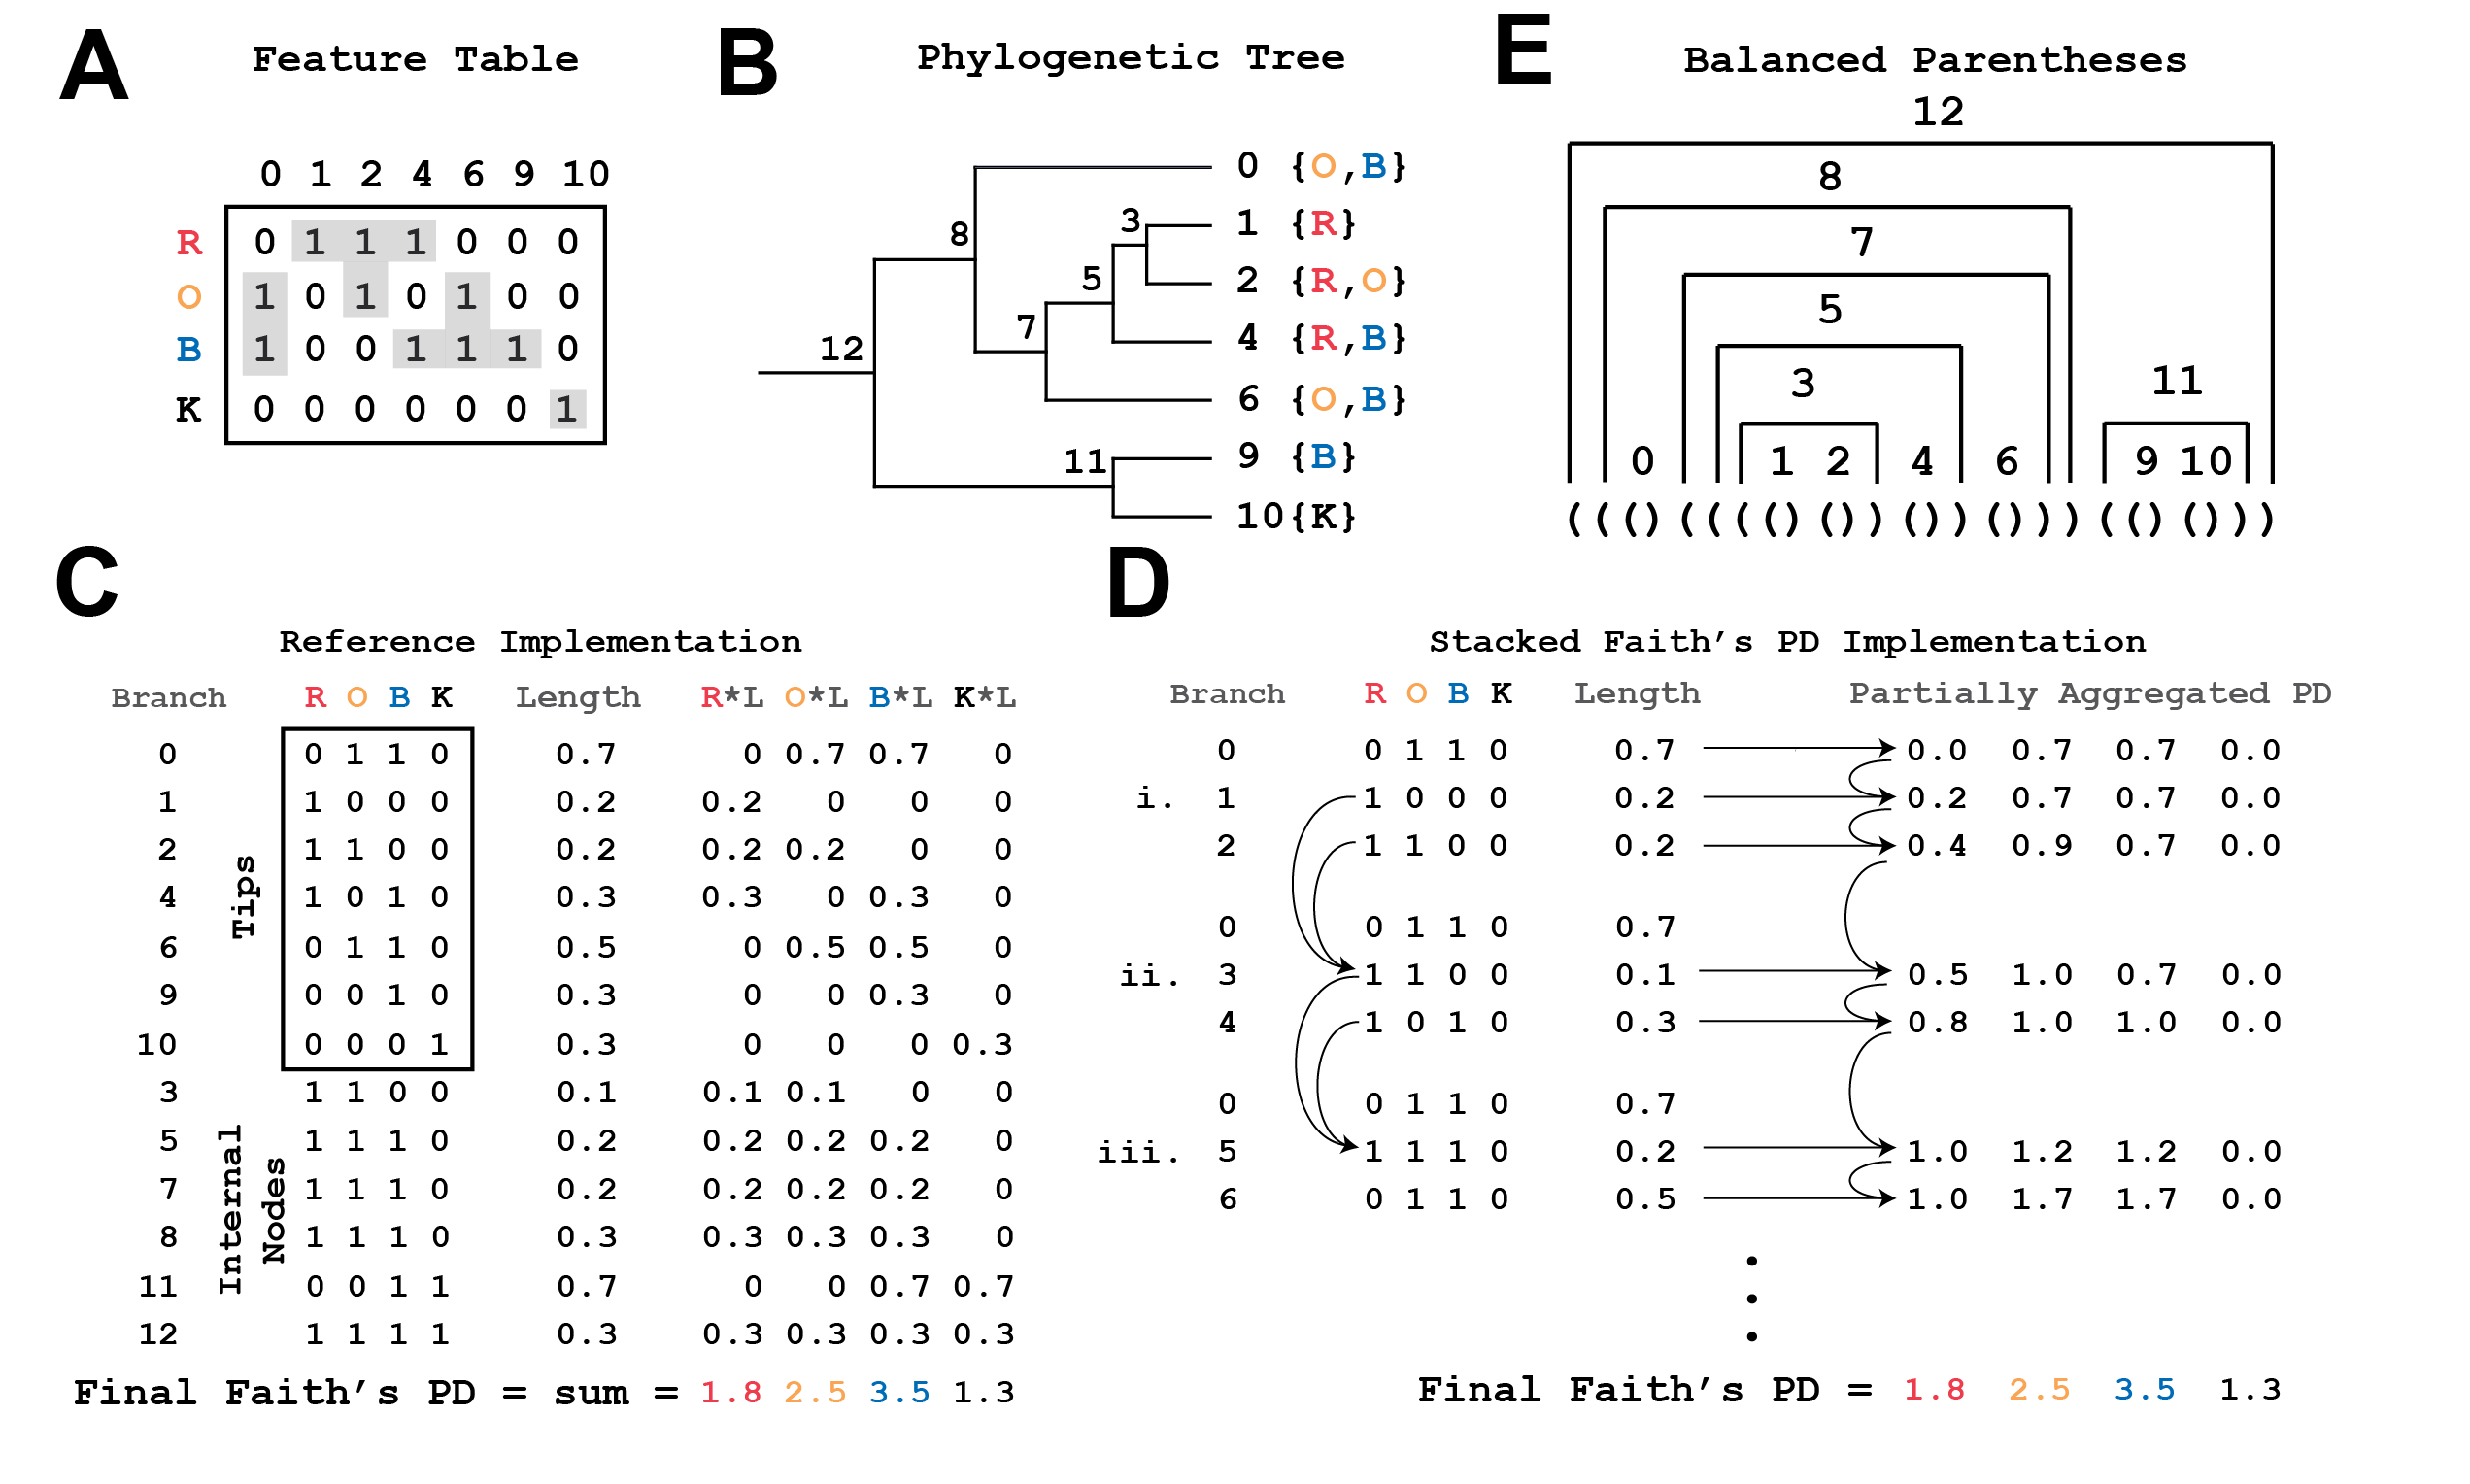
\includegraphics[width=\textwidth]{faiths-pd-figures/figure01.png}
\caption[Partially aggregating branch lengths reduces the space complexity of the algorithm.]{\textbf{Partially aggregating branch lengths reduces the space complexity of the algorithm.} (A) Faith's PD calculation depends on the representation of features present in samples. In the table, the letters (R, O, B, K) represent samples and the numbers (0, 1, 2, 4, 6, 9, 10) represent features. A 1 in an entry indicates the presence of a feature in the sample. SFPhD uses sparse table data structures, which reduce memory by only keeping track of the non-zero values in a matrix (highlighted in gray). (B) A mock reference phylogenetic tree is shown, with the features from (A) as tips. Labels for the samples from (A) are located next to tips that they contain. The nodes are labeled by their order in a post-order traversal of the tree. (C) Graphic depiction of the reference implementation's calculation of Faith's PD by first aggregating the presence/absence information for each branch in the tree, followed by multiplication by the branch lengths to get the metric constituents, and finally a sum over the entire branch ×metric constituent table. (D) Graphic representation of the execution of SFPhD. On the left, the stack of presence/absence information is shown at three points during the algorithm's execution (i, ii, ii). Each of these times shows the stack immediately before memory is freed. On the right, the state of the partially aggregated phylogenetic diversity (PD) is shown after each node is added to the stack. Each row represents the vector after a step in the algorithm. In practice, there is only one such vector. (E) The balanced parentheses representation for the phylogenetic tree from (B).}
\label{faiths_pd_fig1}
\end{figure}

We introduce Stacked Faith’s PD (SFPhD), a novel algorithm and implementation to compute Faith’s Phylogenetic Diversity that uses the structure of microbiome data along with other practical considerations to achieve decreased time and memory requirements. An example feature table is shown in Figure~\ref{faiths_pd_fig1}A, with a corresponding phylogenetic tree in Figure~\ref{faiths_pd_fig1}B. Note that for a given tree $\mathcal{T}$, Faith's PD can be expressed as
\begin{align}
PD_i = \sum_{j\in \mathcal{T}} I_{ij} \times \text{branchLen}_{j}(\mathcal{T})
\end{align}
where $PD_i$ is Faith's PD for sample $i$, $I_{ij}$ indicates if sample $i$ has any features that descend from node $j$, and $\text{branchLen}_j(\mathcal{T})$ indicates the length of the branch to node $j$ in the tree $\mathcal{T}$.

The previous state-of-the-art reference implementation (\href{http://scikit-bio.org/}{scikit-bio}) computes Faith's PD for a batch of samples by first fully computing $I_{ij}$. $I_{ij}$ is computed by traversing the entire phylogenetic tree in a post-order traversal and setting all $I_{ij}$ for a given node $j$ by determining the features present in all children of node $j$. Subsequently, the $I_{ij} \times \text{branchLen}_j(\mathcal{T})$ for all branches is calculated. The final results are obtained by summing over the branches for each sample (Figure~\ref{faiths_pd_fig1}C). However, this approach tends to use much more space than is actually needed.

Microbiome data are known to be sparse \cite{Martino2019-op,Kumar2018-or,Morton2017-bs}, i.e., of the entries in a data table, many are likely to be zero. This issue is exacerbated in large datasets, where many microbes are only observed in a handful of samples. In extreme cases, such as the table from \cite{McDonald2018-qq} with 113,721 samples rarefied at 500 sequences per sample, 0.0126\% of the entries are non-zero. Sparse representations have been used previously for storing microbiome data \cite{McDonald2012-go}, and have been applied for accelerating microbiome analyses \cite{McDonald2018-qq}, however, they have not been previously applied to Faith’s PD. We identified that a major downfall of the state-of-the-art implementation in scikit-bio is that it uses a full, dense table to represent all of $I_{ij}$ in memory at once. A key advancement of our approach is to use a sparse matrix implementation for storing information on the taxa present for each sample and feature (Figure~\ref{faiths_pd_fig1}A). 

Another key advancement is the partial aggregation of Faith's PD (Figure~\ref{faiths_pd_fig1}D). Note that the $I_{ij} \times \text{branchLen}_j(\mathcal{T})$, which we will call a metric constituent, can be added in any order, and that $I_{ij}$ only depends on the children of node $j$. Thus, if node $k$ is a child of node $j$, $I_{ik}$ is no longer needed once metric constituents for node $k$ have been computed and $I_{ij}$ is known. As a result, we can reduce the memory used to store $I_{ij}$ by traversing the phylogeny with a post-order traversal and freeing $I_{ik}$ after they are no longer needed. Furthermore, we can reduce the storage needed for the metric constituents keeping a running summation of them while traversing the tree. Thus, this approach reduces the expected space complexity for storing the metrics from $O(n k)$, to $O(n \log(k))$, where $n$ is the number of samples and $k$ is the number of vertices in the tree.

In addition to the algorithmic improvements, we have included a number of practical enhancements that improve the performance of the code. The phylogenetic tree (Figure~\ref{faiths_pd_fig1}B) is now represented as balanced-parentheses (Figure~\ref{faiths_pd_fig1}E); this structure has a lower memory footprint and a sequential memory representation which reduces the number of cache misses during a tree traversal \cite{Cordova2016-vf}. Finally, the software is written using C/C++ (with Python extensions using Cython, https://cython.org/) and builds upon the foundation established by Striped UniFrac \cite{McDonald2018-qq}. Reuse of this library facilitated our access to a much faster Newick format parser, which reduces the overhead when reading a tree from disk. These factors make for an improved expected and in-practice performance, despite the time complexity and worst-case memory complexity remaining the same.

To demonstrate the scalability of SFPhD, we used a collection of 307,237 public and anonymized private 16S rRNA V4 microbiome samples amounting to 1,264,796 phylogenetic tree tips (after rarefaction at 500 sequences per sample). The samples were retrieved using the redbiom command line interface \cite{McDonald2019-th} which queried a cache of public and anonymized private studies available in Qiita \cite{Gonzalez2018-ez}. Amplicon sequence variants (ASVs) were placed into the Greengenes \cite{Gonzalez2018-ez,McDonald2012-zv} phylogeny using SEPP \cite{Mirarab2012-jh}. Computing the full alpha diversity vector took SFPhD 1 hour and 5 minutes wall-clock time and required a maximum resident set size of less than 3 GB (see Methods for hardware details). In addition, we iteratively measured runtime and memory consumption for increasingly large random subsets of samples while fixing the size of the tree at 100,000 tips (Figure~\ref{faiths_pd_fig2} A,B). For the iteration with 20,000 samples, the memory usage of the reference implementation exceeded 150 GB and the process ran for over 15 minutes. Contrastingly, with SFPhD, the process took 14 seconds to execute and required less than 0.5 GB of memory. Additionally, using  Green Algorithms \cite{Lannelongue2021-vg}, we estimated the carbon footprint of the scikit-bio reference implementation on the 20,000 sample table be 12.84 g CO2e, whereas we estimated the carbon footprint of SFPhD would be 0.04 g CO2e in the United States, which is a 321-fold reduction in impact on global warming.

\begin{figure}[htbp]
\centering
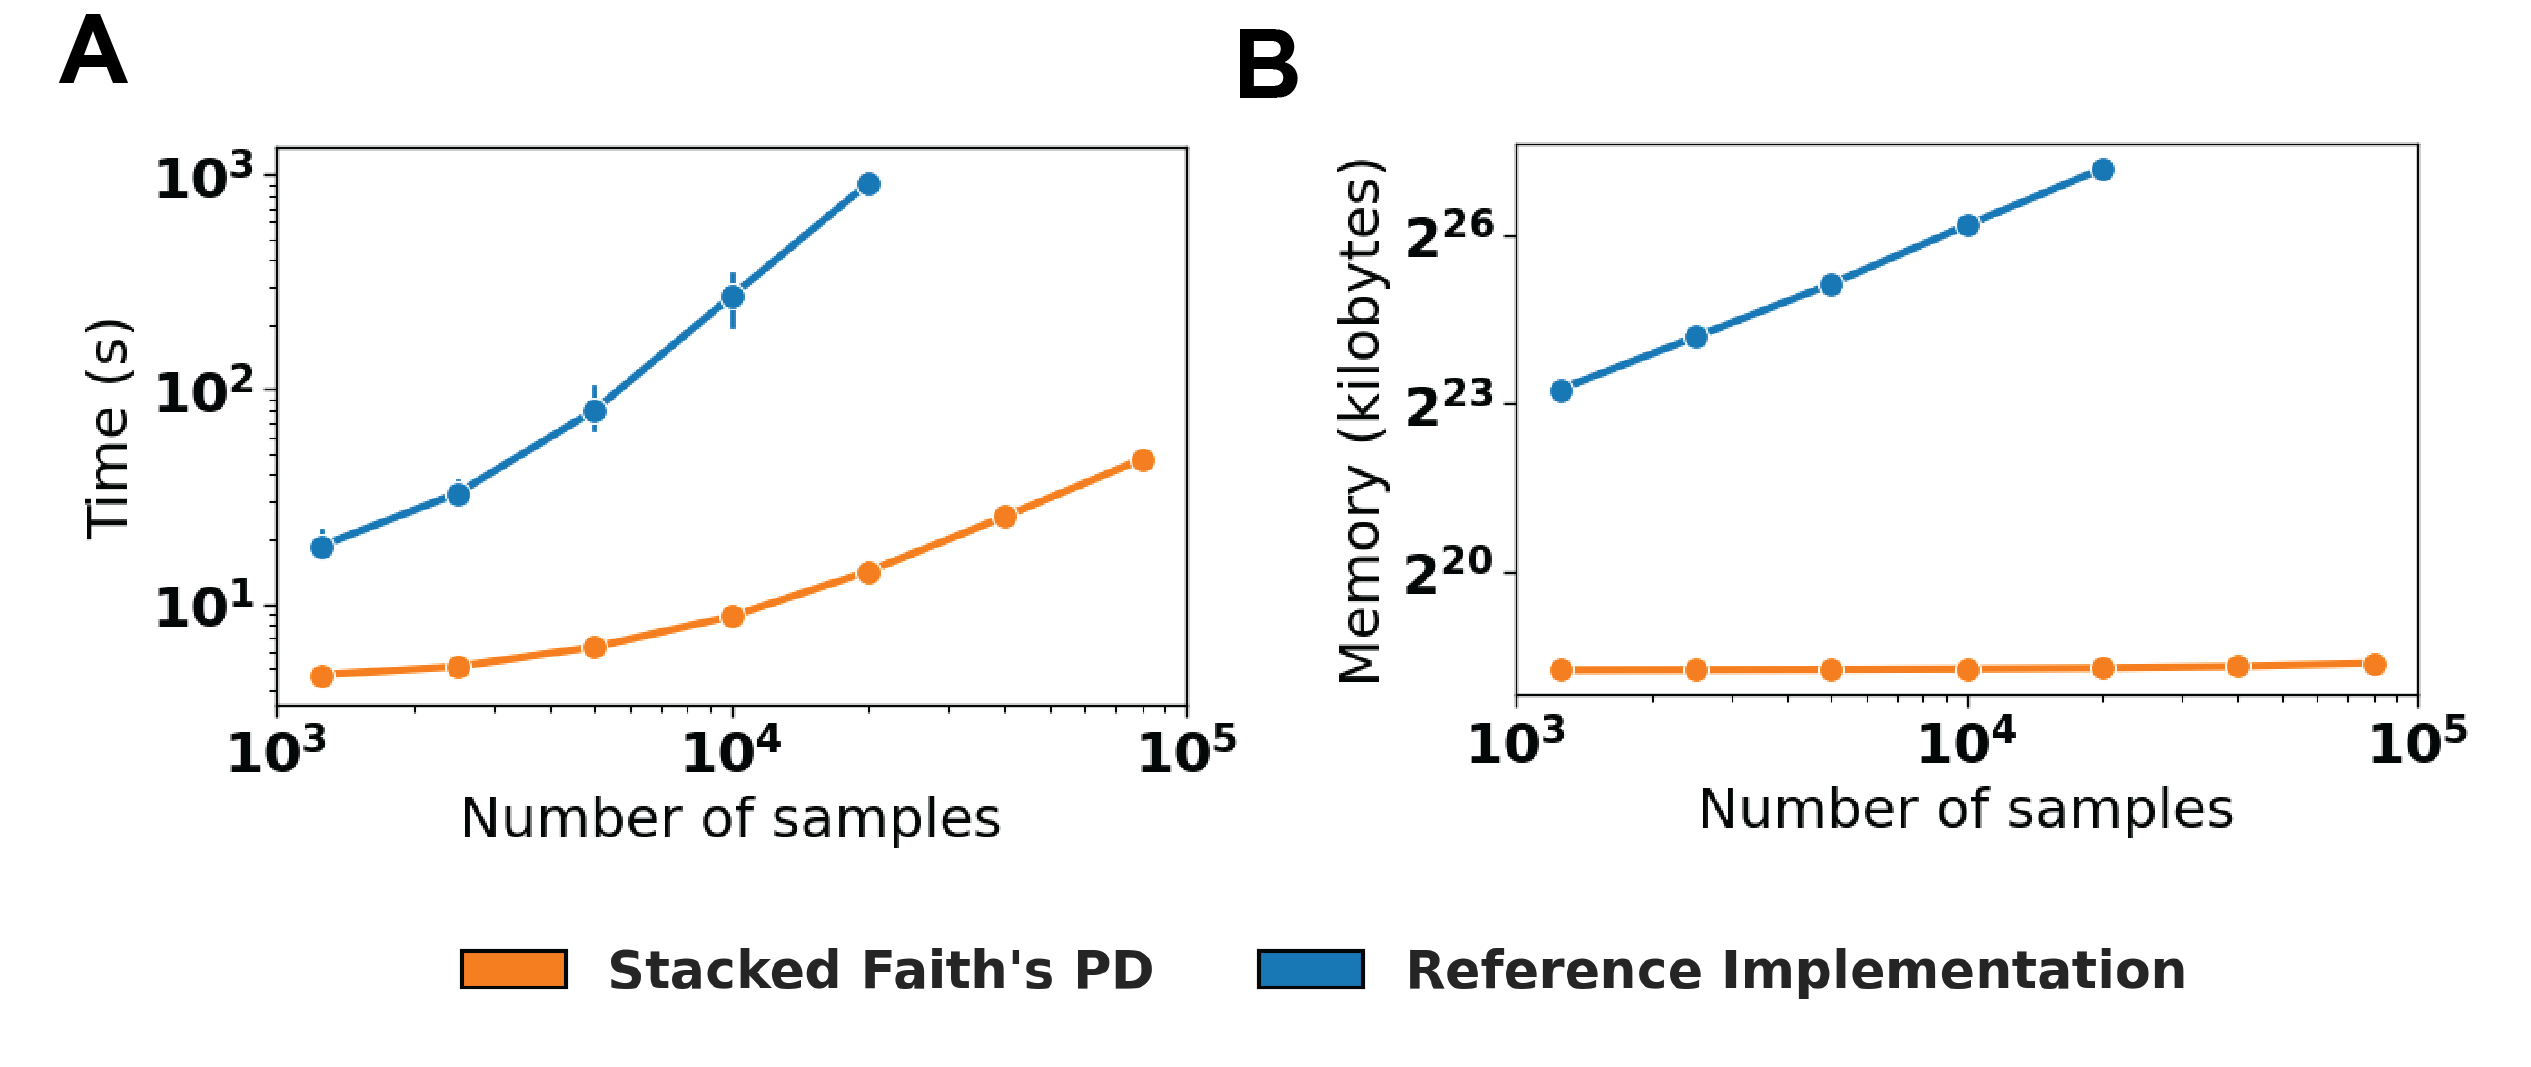
\includegraphics[width=\textwidth]{faiths-pd-figures/figure02.png}
\caption[SFPhD outperforms the reference implementation in terms of runtime and memory usage.]{\textbf{SFPhD outperforms the reference implementation in terms of runtime and memory usage.} (A) Runtime in seconds for computing Faith’s PD on datasets with thousands of samples and 100,000 tips in the phylogeny. Data is independently sub-sampled from a collection of 113,721 public samples in Qiita \cite{Zhu2019-od, Gonzalez2018-ez} as previously processed \cite{McDonald2018-qq}. Mean of n=10 repetitions with 95\% CI error bars. (B) Memory usage for the same experiment as in (A). For both a and b jobs were terminated if they exceeded 250 GB of memory.}
\label{faiths_pd_fig2}
\end{figure}

\subsection{Phylogenetic diversity is a suitable metric to analyze stool metagenomic samples}

To demonstrate SFPhD’s versatility and applicability to newer datasets, we reanalyzed 2,661 paired 16S rRNA and metagenomic data of stool samples from the FINRISK \cite{Borodulin2015-uz,Salosensaari2020-tx,Borodulin2017-sx} study (n=1,563 aged 60 and older, n=1,098 aged 35 and under) \cite{Salosensaari2020-tx,Borodulin2015-uz}. In this experiment, we select random subsets of the full sample set and compare each metric’s (Observed Features and Faith’s PD) ability to detect differences in mean alpha diversity distributions. For each step we randomly select $N$ paired 16S and metagenomic samples, and then compute the difference in mean alpha diversity between samples taken from younger adults (under 35 years) and older adults (over 60 years) together with an empirical p-value. For both 16S and metagenomics, the alpha diversity of younger adults is lower than in older adults. In metagenomics, but not in 16S sequencing, Faith’s PD provides improved statistical power over a phylogenetically-agnostic alternative (Figure~\ref{faiths_pd_fig3} A,B). With 16S data, the difference between the two metrics is subtle (Figure~\ref{faiths_pd_fig3}A). In both cases, the statistical power increases as the number of samples grows. With metagenomic data, the number of observed features shows a weaker effect compared to Faith’s PD regardless of the number of samples (Figure~\ref{faiths_pd_fig3}B). Unlike 16S datasets (5,600 features), metagenomic datasets (1,700 features) are resolution-limited by the reference databases. Whereas the nature of amplicon sequence variants (ASVs) allow for a broader feature space that can capture age-differences without the need for a phylogeny. 

\begin{figure}[htbp]
\centering
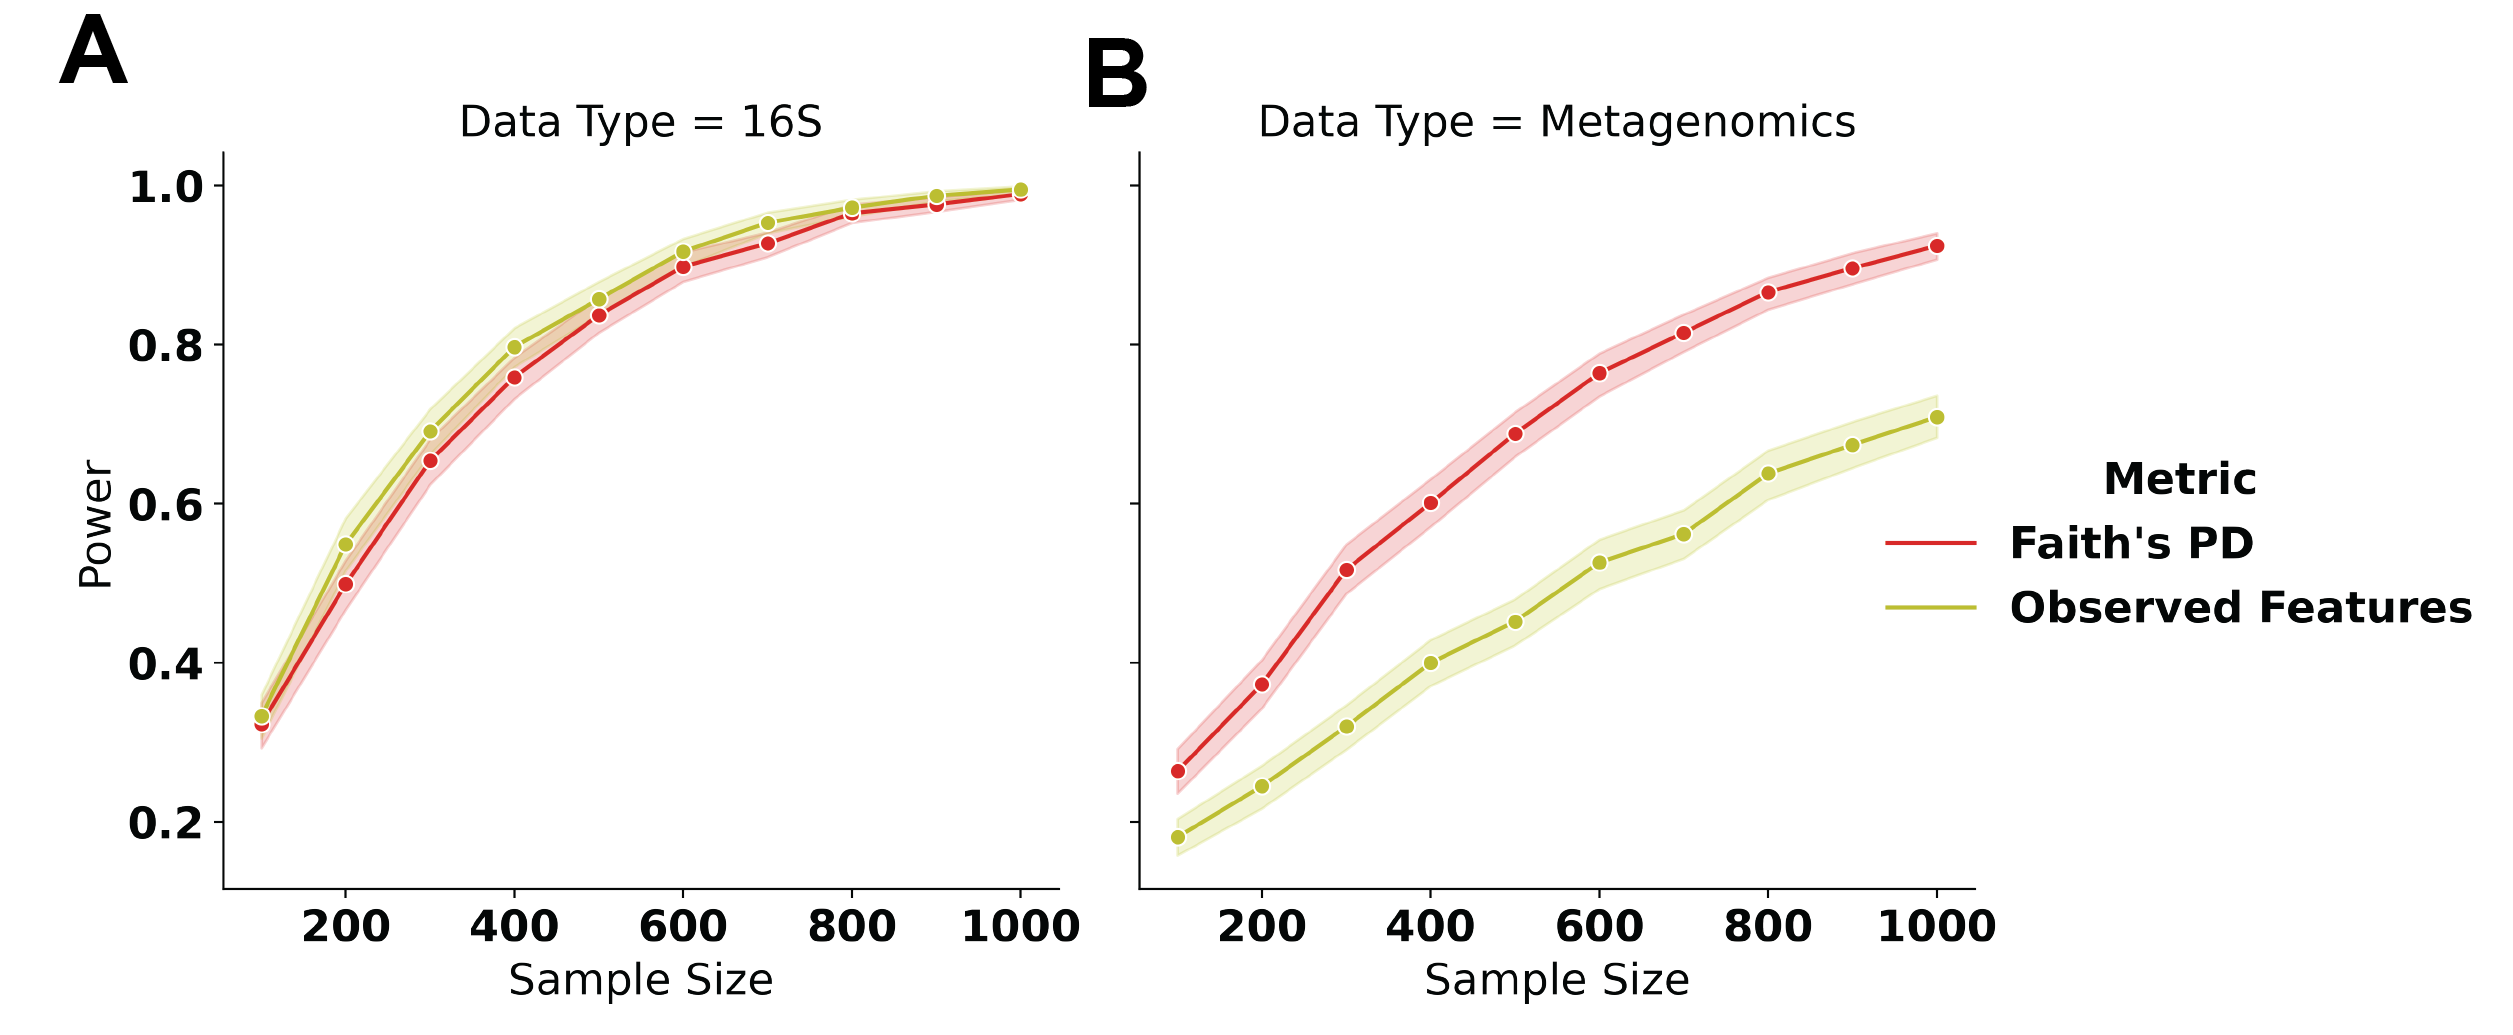
\includegraphics[width=\textwidth]{faiths-pd-figures/figure03.png}
\caption[Phylogenetic diversity provides increased statistical power to differentiate age groups in shotgun metagenomics but not in 16S rRNA sequencing.]{\textbf{Phylogenetic diversity provides increased statistical power to differentiate age groups in shotgun metagenomics but not in 16S rRNA sequencing.}  (A) Statistical power to differentiate young adults from old adults in two alpha diversity metrics at different sample sizes using 16S rRNA sequencing in the FINRISK cohort. (B) Same as (A) but for shallow shotgun metagenomic sequencing.}
\label{faiths_pd_fig3}
\end{figure}

By computing the log of the likelihood ratio of older to younger adult samples present for each branch in the WoL phylogenomic tree \cite{Zhu2019-od}, we were able to identify portions of the WoL tree responsible for the increase in phylogenetic diversity (Figure~\ref{faiths_pd_fig4}B). From this analysis, we found that the majority of the tree is comparably represented in young and old adult samples. However, we also found two clades where older adult samples were more prevalent than younger adult samples (Clade 1 has a log ratio bounded with an 80\% confidence interval of [1.20, 1.45] and Clade 2 has an 80\% confidence interval of [0.55, 0.74]). Clade 1 corresponds to a majority of \textit{Lactobacillales} genomes, and Clade 2 corresponds to \textit{Proteobacteria} genomes. The branches in Clade 1 primarily have a large log likelihood ratio, indicating that the features across the entire clade are more likely to be found in samples from older adults. However, the internal branches in Clade 2 additionally have low log likelihood ratios, indicating that the enrichment of features in older adults is not completely consistent across the entire clade. Lastly, although not confined to a few clades, there are several tips (e.g. \textit{Staphylococcus aureus}, \textit{Bavariicoccus seileri}, \textit{Nitratireductor indicus}, and \textit{Campylobacter ureolyticus}) in the phylogeny that are only associated with younger adults.

\begin{figure}[htbp]
\centering
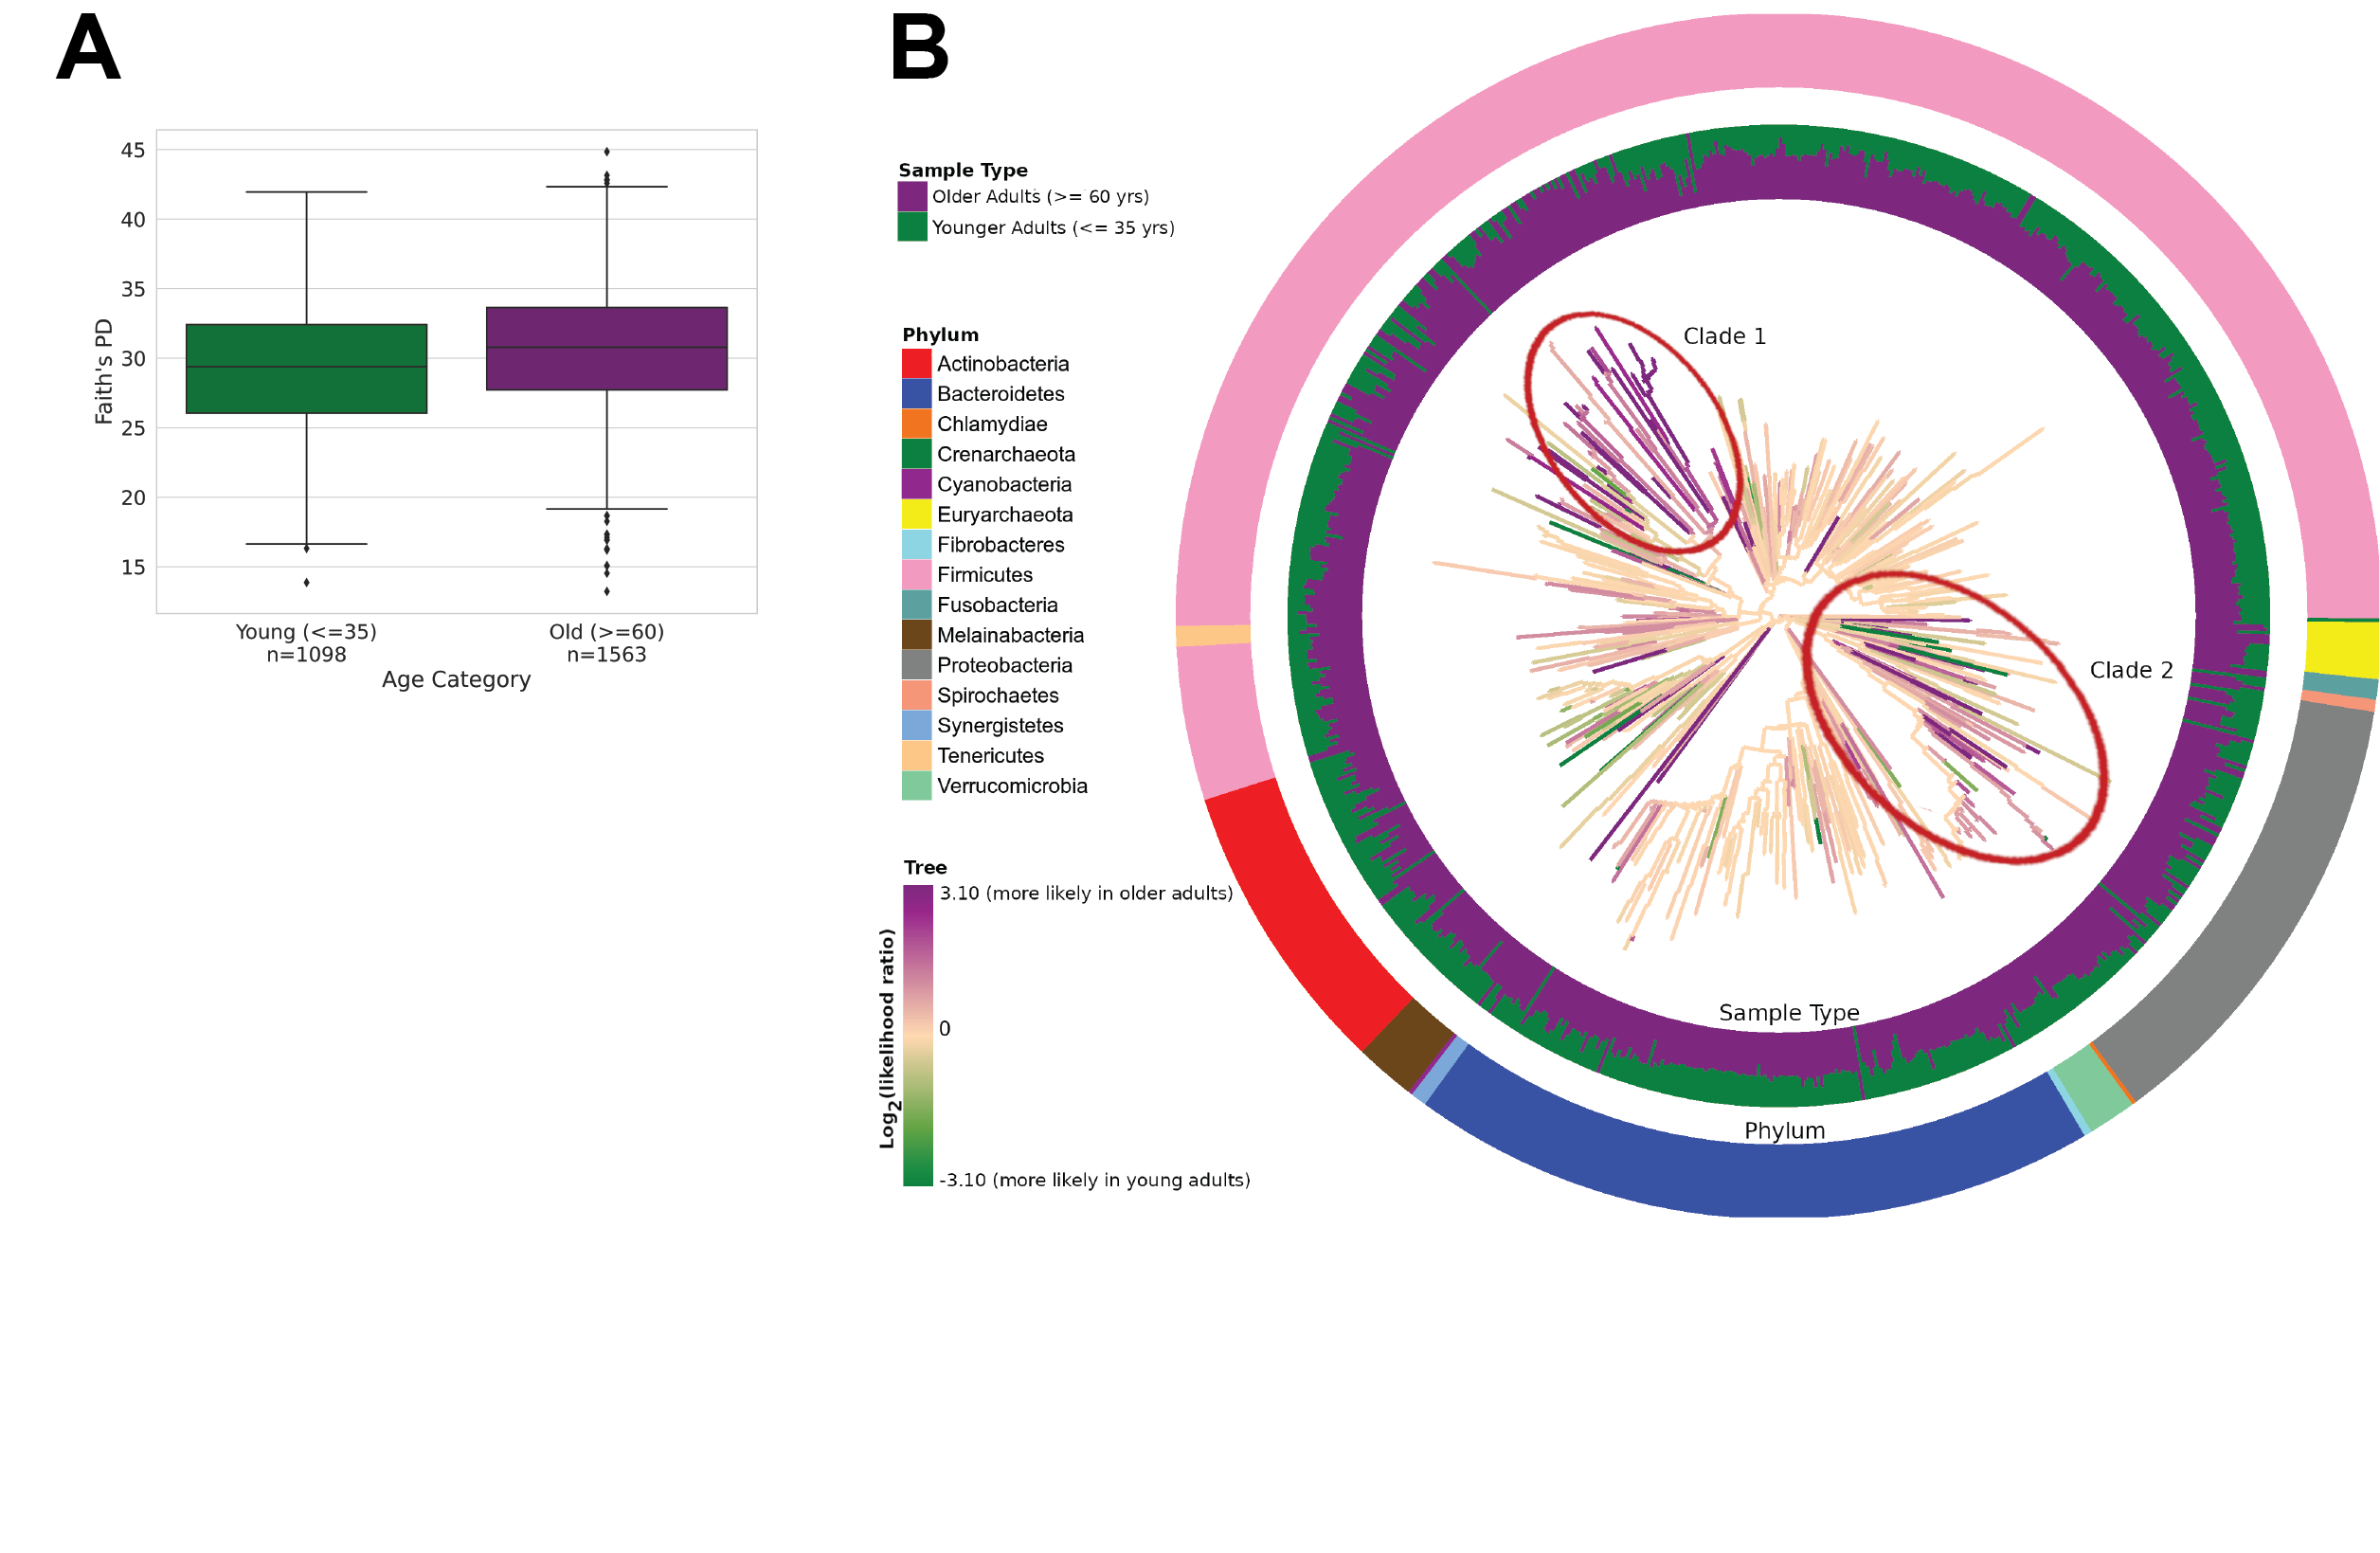
\includegraphics[width=\textwidth]{faiths-pd-figures/figure04.png}
\caption[Phylogenetic tree colored by age-group log of the likelihood ratio of older to younger adults per node]{\textbf{Phylogenetic tree colored by age-group log of the likelihood ratio of older to younger adults per node.}  (A) Distribution of Faith's PD by age group on the full dataset. (B) Web of Life (WoL) Phylogenetic tree with branches colored by the log of likelihood ratio of old adults compared to young adults in descendants of the branch, for the FINRISK dataset. The inner circle is colored by the log of likelihood ratio of older adults compared to younger adults in the tips of the tree. The outer circle is colored by the phylum of the taxon represented by each tree tip. Red ellipses mark two clades enriched for samples from older individuals.}
\label{faiths_pd_fig4}
\end{figure}

\section{Discussion}
By accounting for the relationship between features in a dataset, Faith’s PD is able to mitigate issues with sparsity and heterogeneity common to modern `omics’ datasets. Although this metric was first introduced 30 years ago, the underlying algorithm for computing this metric had largely remained unchanged. In this paper we demonstrated that our novel algorithm, SFPhD, performed efficiently on datasets with hundreds of thousands of samples and millions of tree tips.

An important aspect of SFPhD’s underlying algorithm is substituting calculation of the full presence/absence table over the phylogeny, for a tree traversal that partially aggregates diversity values and frees presence/absence information when no longer needed. The result is a high-performance implementation that demonstrates improved scaling, with the number of samples in the input dataset. Much of the engineering work here was facilitated by the balanced parenthesis tree implementation provided in the UniFrac package \cite{McDonald2018-qq}. Therefore, we believe that increasing the availability of efficient and flexible data structures for bioinformatic analyses, is likely to accelerate and facilitate the development of novel analytical methods. In a broader sense, this is similar to the impact of NumPy’s \cite{McDonald2018-qq,Harris2020-vb} N-dimensional array in image processing, machine learning, neuroscience, and other fields. 

In addition, in a stool metagenomic study Faith’s PD demonstrates increased statistical power compared to Observed Features for differentiating younger from older subjects based on their microbial communities. In this context, we show that while the choice of alpha diversity metric did not make a significant difference for the 16S dataset in this study, Faith's PD consistently provided increased statistical power for determining age-based differences in the shotgun metagenomic sequencing data. While this metric was originally developed to analyze data with vastly different statistical and biological properties, its use here demonstrates the versatility and applicability behind measuring diversity using a tree. Although we show the utility of SFPhD in large and complex microbiome studies, the underlying implementation is not tied to a particular molecular technology. Thus, we envision that this implementation will be relevant to fields outside of microbiology, like nutrition and metabolomics research, that only recently began adopting trees for analytical tasks \cite{Tripathi2021-wf,Johnson2019-nx}.  

\section{Methods}
\subsection{Construction of benchmarking tables}
Data for the benchmarking in this study were subsampled from a BIOM table of 113,721 and 761,003 ASVS, which is composed of studies aggregated from several large sources of publicly available microbiome data in Qiita \cite{Amir2017-sk,Gonzalez2018-ez}. This data table was produced as in \cite{McDonald2018-qq}. The data was subset by uniformly randomly sampling the desired number of ASVs and samples from the table. Ten different tables were created for each number of samples and ASVs. The insertion tree from \cite{McDonald2018-qq} was collapsed to only contain sequences that were selected to be included in the given subsampled table.
The table with 307,237 public and anonymized private 16S rRNA V4 microbiome samples and 1,264,796 phylogenetic tree tips was also prepared as in \cite{McDonald2018-qq}, but included samples with private sequencing data from Qiita.

\subsection{Benchmarking time and memory estimates
}

The SFPhD implementation available in the python package unifrac v0.10.0 was used. The reference implementation uses the Faith's PD implementation from scikit-bio v0.5.4.

All methods were run single-threaded on shared compute nodes that were not running other compute tasks. The nodes all had Intel(R) Xeon(R) CPU E5-2640 v3 @ 2.60GHz processors. A job was terminated if it exceeded 6 hours of wall time or 250 GB of memory (system max). Space was tracked using GNU Time. Time for both implementations was tracked with a python wrapper script. The time needed to parse data is not included in the scikit-bio timings, but is included in the SFPhD timings, due to the lack of access to this information in the unifrac interface. This is acceptable given that it results in a conservative estimate of the speedup with SFPhD.

\subsection{Carbon footprint estimation}
The Green Algorithms interface \cite{Lannelongue2021-vg} was used to estimate the Carbon Dioxide equivalent ($\text{CO}_2\text{e}$) of the benchmarked methods. The Intel(R) Xeon(R) CPU E5-2640 v3 CPUs used in benchmarking have a Thermal Design Power (TDP) per core of the  11.25 TDP / core.

\subsection{FINRISK processing}
The 16S rRNA data were demultiplexed, quality filtered, and denoised with deblur \cite{Amir2017-sk}.The Greengenes \cite{McDonald2012-zv} 13.8 with a clustering level of 99\% was used as the reference phylogeny for open-reference feature picking with SEPP \cite{Mirarab2012-jh}. ASVs with a total frequency fewer than 10 were discarded, and the table was then rarefied to a sampling depth of 1000 reads/sample. The resulting table and insertion tree were used for calculation of Faith's PD.
The shotgun metagenomic data were trimmed and quality filtered using Atropos \cite{Didion2017-pl}. They were aligned to the WoL database using SHOGUN pipeline (v1.0.8) with a Bowtie2 alignment option. A table was generated from the alignments using the OGU workflow \cite{Zhu2021-ap}.  OGUs with a total frequency fewer than 10 were discarded, and the table was then rarefied to a sampling depth of 1000 reads/sample. The WoL phylogenomic tree \cite{Zhu2021-ap,Zhu2019-od} was used for Faith's PD.
Both tables were filtered to include only samples from individuals 35 and younger (younger criteria) or 60 and older (older criteria).

\subsection{Power estimation for mean difference in alpha diversity}
For a given $N$ (shown on horizontal axis in Figure~\ref{faiths_pd_fig3} A,B), the FINRISK processed samples matching the younger/older criteria were sampled to this depth. On the subsampled data, the difference in mean alpha diversity between younger and older adults $\bar{d}$, was computed. A null distribution, $\hat{D}$, was generated by repeating 1000 repetitions of shuffling the  age category associated with an alpha diversity and recomputing the difference of mean alpha diversity between the groups. The p-value was computed by finding the percentile of $\bar{d}$ in $\hat{D}$.
This test procedure was repeated for 1000 repetitions. The power for $N$ is estimated as the proportion of tests found significant at $\alpha = 0.05$.

\subsection{Phylogenetic Visualization}
Tree was visualized using EMPress \cite{Cantrell2021-mx}. A node in the tree was considered old if its $\text{age}_{\text{log}} > 0$ and young if its $\text{age}_{\text{log}} < 0$.

\section{Data Access}
The data used for benchmarking Faith's PD timing and memory usage are available as per the Striped UniFrac paper \cite{McDonald2018-qq}. The code for the benchmarking is available on GitHub (https://github.com/biocore/faiths-pd-benchmarking). The data and code needed for benchmarking the FINRISK metagenomics data are also available on GitHub. The SFPhD code is available in the unifrac python package (https://github.com/biocore/unifrac). 

\section{Acknowledgements}
This work was supported in part by IBM Research AI through the AI Horizons Network, the Center for Microbiome Innovation at UC San Diego, the Academy of Finland grant 321351 and the Emil Aaltonen Foundation (to T.N.), the National Institutes of Health grant R01ES027595 (to M.J.), the Academy of Finland grants 321356 and 335525 (A.S.H), the Academy of Finland grant 295741 (L.L.). MI was supported by the Munz Chair of Cardiovascular Prediction and Prevention. VS was supported by the Finnish Foundation for Cardiovascular Research. 

Chapter~\ref{chapter_faiths_pd}, in full, is a reprint of the material as it appears in ``Efficient computation of Faith's phylogenetic diversity with applications in characterizing microbiomes.'' George Armstrong, Kalen Cantrell, Shi Huang, Daniel McDonald, Niina Haiminen, Anna Paola Carrieri, Qiyun Zhu, Antonio Gonzalez, Imran McGrath, Kristen Beck, Daniel Hakim, Aki S Havulinna, Guillaume Méric, Teemu Niiranen, Leo Lahti, Veikko Salomaa, Mohit Jain, Michael Inouye, Austin D Swafford, Ho-Cheol Kim, Laxmi Parida, Yoshiki Vázquez-Baeza and Rob Knight. \textit{Genome Research 31}, 2021. The dissertation author was the primary investigator and the first author of this paper.


\chapter{Uniform Manifold Approximation and Project (UMAP) reveals composite patterns and resolves visualization artifacts in microbiome data}\label{chapter_umap}


\glsresetall

% \section{Abstract}


Microbiome data are sparse and high-dimensional, so effective visualization of these data requires dimensionality reduction. To date, the most commonly used method for dimensionality reduction in the microbiome is calculation of between-sample microbial differences (beta diversity), followed by Principal Coordinates Analysis (PCoA). Uniform Manifold Approximation and Projection (UMAP) is an alternative method that can reduce the dimensionality of beta diversity distance matrices. Here, we demonstrate the benefits and limitations of using UMAP for dimensionality reduction on microbiome data. Using real data, we demonstrate that UMAP can improve the representation of clusters, especially when the clusters are composed of multiple subgroups. Additionally, we show that UMAP provides improved correlation of biological variation along a gradient with a reduced number of coordinates of the resulting embedding. Finally, we provide parameter recommendations that emphasize the preservation of global geometry. We therefore conclude that UMAP should be routinely used as a complementary visualization method for microbiome beta diversity studies.


\section{Importance}
UMAP provides an additional method to visualize microbiome data. The method is extensible to any beta diversity metric used with PCoA, and our results demonstrate that UMAP can indeed improve visualization quality and correspondence with biological and technical variables of interest. The software to perform this analysis is available under an open-source license and can be obtained at https://github.com/knightlab-analyses/umap-microbiome-benchmarking; additionally, we have provided a QIIME 2 plugin for UMAP at\\ https://github.com/biocore/q2-umap.

\section{Observation}
An important step in microbiome research is visualizing the relationships between samples. In the study of microbial communities through next generation sequencing (NGS), these comparisons are typically done through the visualization of beta diversities with principal coordinates analysis (PCoA) \cite{Kruskal1978-xx} (Figure~\ref{umap_figS1}). Although alternatives such as conventional principal component analysis (PCA), non-metric multidimensional scaling  (NMDS) \cite{Kruskal1964-dn} and t-distributed stochastic neighbor embedding (t-SNE) \cite{Van_der_Maaten2008-af} are sometimes applied, PCoA in particular has been widely adopted by the microbiome community.  Due to the high dimensional and highly sparse nature of the data, which presents challenges on sequence count data \cite{Aitchison1983-mz,Martino2019-op}, one major benefit of PCoA over other methods on untransformed count data is that it accommodates a generalized distance matrix (of beta diversities, for the microbiome).  This allows use of distance metrics that are better-suited for sparse data (e.g., Bray-Curtis \cite{Bray1957-fg}, Jaccard \cite{Jaccard1912-bk}, UniFrac \cite{Lozupone2005-aj}).
Uniform Manifold Approximation and Projection (UMAP) \cite{McInnes2018-zd}  is a method that has gained traction in single-cell genomics analysis \cite{Hao2020-gu}. Whereas PCoA performs an eigendecomposition that focuses on linearly preserving the pairwise distances between the samples (global structure), UMAP uses a non-linear graph construction and embedding method to optimize an objective that allows for a trade-off between emphasizing local structures and preserving distances globally. This trade-off is primarily controlled by the `n\_neighbors' and `min\_dist' parameters of UMAP. The `n\_neighbors' parameter controls the number of neighbors whose local topology is preserved, so global distances are preserved when it is high. The `min\_dist' parameter controls the minimum distance between samples in the embedding, which affects the spread of clusters. Low values of `min\_dist' allow UMAP to emphasize the similarity of dense clusters of samples, whereas larger values of `min\_dist' will focus on preserving distances more broadly.
Both UMAP and PCoA operate on a generalized distance (beta diversity) matrix, appropriate for microbiome data (Figure~\ref{umap_figS1}). While the use of UMAP on microbiome data has been noted (11) the utility of UMAP on microbiome data remains underexplored. Using real datasets, we compared both visual qualities and quantitative measures of UMAP to PCoA on well understood datasets. We additionally applied UMAP to data from the Human Microbiome Project (HMP) \cite{The_Human_Microbiome_Project_Consortium2012-og} to demonstrate its characteristics on a larger dataset with more complex sources of variation.
Discrete clusters are one common pattern that microbial communities can exhibit \cite{Kuczynski2010-gu}. The `keyboard data' from \cite{Fierer2010-dp} contains 16S samples (n = 99, features  = 1399, 5\% dense) from the keyboards and fingers of 3 subjects. PCoA on the Aitchison distances on these samples can recover the cluster structure of the subjects in the data (Figure~\ref{umap_fig1}A). We compared this to UMAP (n\_neighbors = 15 and n\_neighbors = 80, min\_dist = 1) and found that UMAP can also recover the cluster structure of the subjects (Figure~\ref{umap_fig1} B,C). We also saw that UMAP produced two-dimensional coordinates with improved separation within subjects by sample type. This was further supported by improved LDA classification of sample type stratified by subject (Table~\ref{umap_table1}).


\begin{figure}[htbp]
\centering
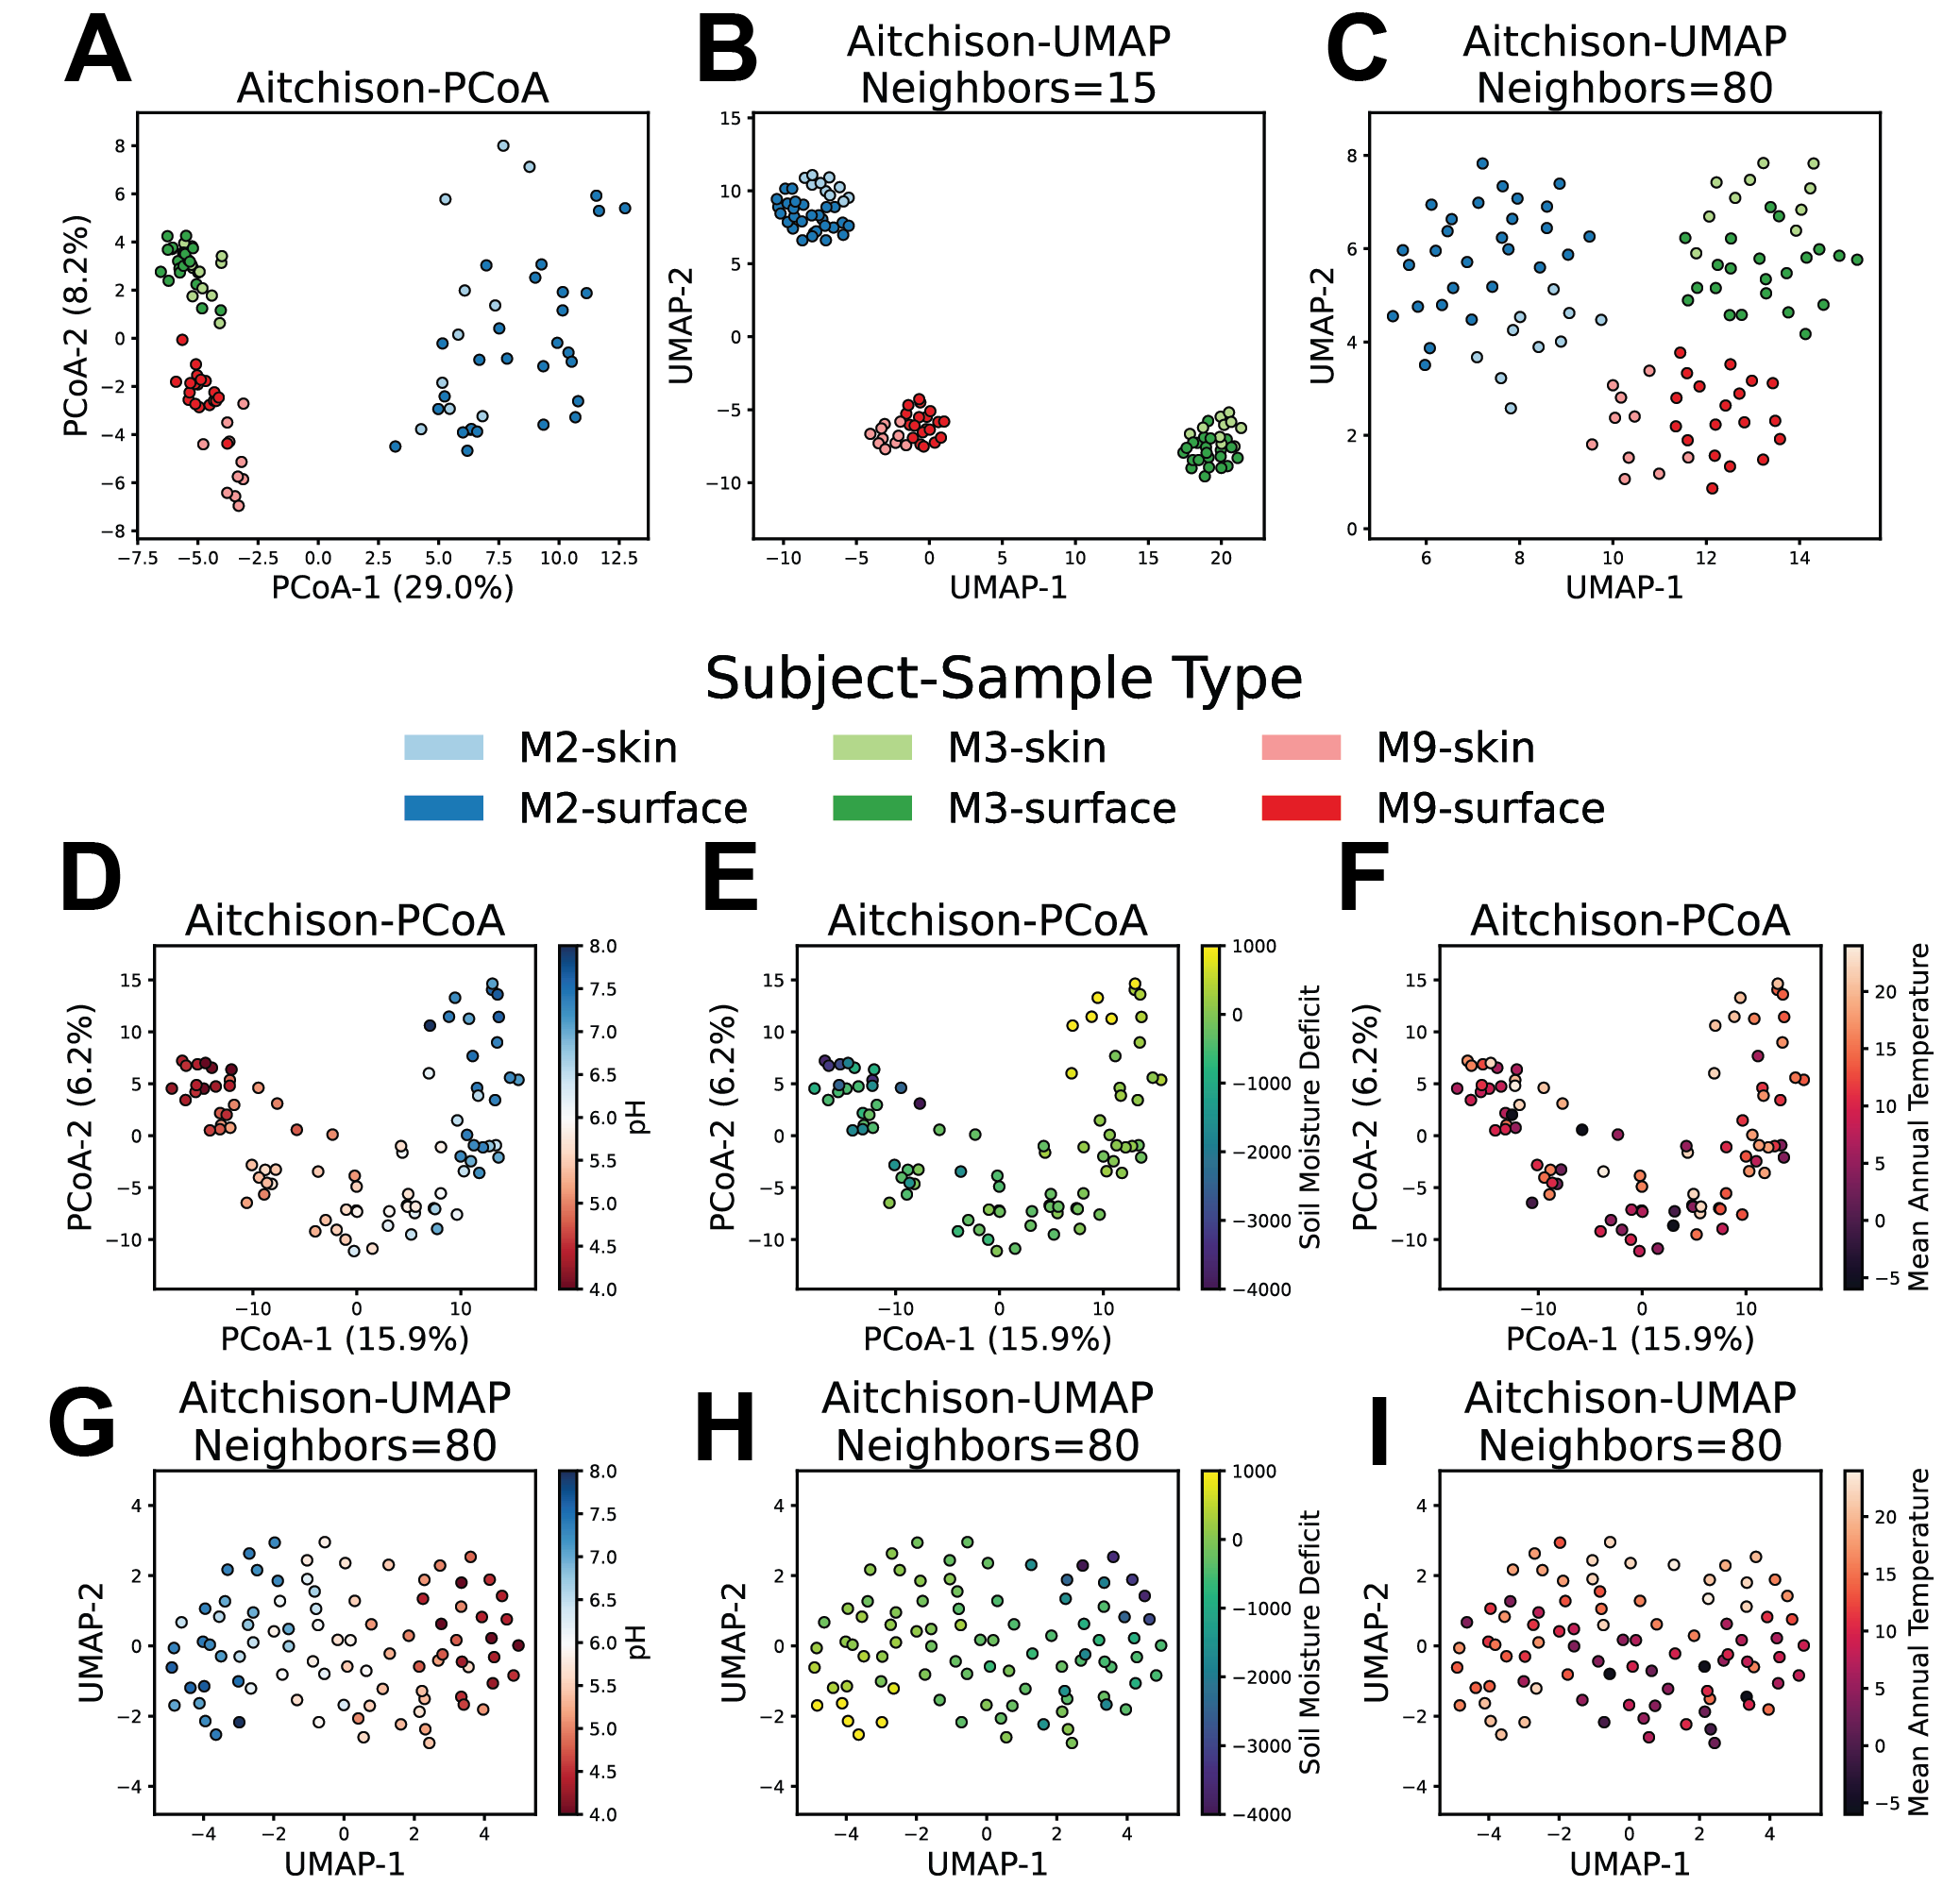
\includegraphics[width=0.8\textwidth]{umap-figures/figure01.png}
\caption[Comparison of PCoA and UMAP visualizations of cluster and gradient patterns on real data.]{\textbf{ Comparison of PCoA and UMAP visualizations of cluster and gradient patterns on real data. } The keyboard data set contains samples from three different subjects’ keyboards (surface) and their hands (skin). (A) PCoA on Aitchison distances (pseudocount = 1) demonstrates a strong separation between M2 and the other subjects, as well as separation between subjects M3 and M9. (B) A UMAP (n\_neighbors = 15, min\_dist = 1) visualization demonstrates stronger clustering by subject, with a different relative positioning of the clusters by subject. The plot also emphasizes clustering by sample type. (C) UMAP with an increased n\_neighbors parameter (n\_neighbors = 80, min\_dist = 1) reflects the same relative positioning of clusters as PCoA. It also demonstrates the improved localization by sample type within subjects. (D) On the “88 soils” data, PCoA on the Aitchison distances demonstrates a horseshoe pattern with pH distributed along the horseshoe. (E) Soil moisture deficit is also distributed along the horseshoe, and (F) there is not a strong association between mean annual temperature and position on the PCoA. (G) In the UMAP (n\_neighbors = 80, min\_dist = 1), followed by centering/rotation with PCA }
\label{umap_fig1}
\end{figure}

\begin{sidewaystable}[]
\caption{Linear Discriminant Analysis on Aitchison Embedding 10 different initializations for UMAP}
\singlespace
\label{umap_table1}
\centering
\begin{tabular}{llllllll} \hline
\multicolumn{1}{c}{} & \multicolumn{1}{c}{Metric} & \multicolumn{1}{c}{\begin{tabular}[c]{@{}c@{}}PCoA \\ Dims=2\end{tabular}} & \multicolumn{1}{c}{\begin{tabular}[c]{@{}c@{}}PCoA\\ Dims=3\end{tabular}} & \multicolumn{1}{c}{\begin{tabular}[c]{@{}c@{}}UMAP\\ Neighbors=15 \\ Dims=2\end{tabular}} & \multicolumn{1}{c}{\begin{tabular}[c]{@{}c@{}}UMAP\\ Neighbors=80 \\ Dims=2\end{tabular}} & \multicolumn{1}{c}{\begin{tabular}[c]{@{}c@{}}UMAP\\ Neighbors=98\\ Dims=2\end{tabular}} & \multicolumn{1}{c}{\begin{tabular}[c]{@{}c@{}}UMAP\\ Neighbors=98\\ Dims=2\end{tabular}} \\ \hline
\multirow{2}{*}{host} & \begin{tabular}[c]{@{}l@{}}mean\\ (Accuracy)\end{tabular} & 0.990 & 1.000 & 1.000 & 1.000 & 1.000 & 1.000 \\
 & std &  &  & 0.000 & 0.000 & 0.000 & 0.000 \\ \hline
\multirow{2}{*}{M2-type} & \begin{tabular}[c]{@{}l@{}}mean\\ (Accuracy)\end{tabular} & 0.789 & 0.921 & 0.974 & 0.992 & 0.989 & 0.997 \\
 & std &  &  & 0.012 & 0.013 & 0.014 & 0.008 \\ \hline
\multirow{2}{*}{M3-type} & \begin{tabular}[c]{@{}l@{}}mean\\ (Accuracy)\end{tabular} & 0.781 & 0.844 & 0.856 & 0.831 & 0.828 & 0.900 \\
 & std &  &  & 0.049 & 0.059 & 0.065 & 0.041 \\ \hline
\multirow{2}{*}{M9-type} & \begin{tabular}[c]{@{}l@{}}mean\\ (Accuracy)\end{tabular} & 0.931 & 0.966 & 0.990 & 0.969 & 0.972 & 0.976 \\
 & std &  &  & 0.017 & 0.025 & 0.027 & 0.023 \\ \hline
\multirow{2}{*}{host} & \begin{tabular}[c]{@{}l@{}}mean\\ (Silhouette)\end{tabular} & 0.647 & 0.601 & 0.794 & 0.548 & 0.533 & 0.500 \\
 & std &  &  & 0.069 & 0.011 & 0.018 & 0.008 \\ \hline
\multirow{2}{*}{M2-type} & \begin{tabular}[c]{@{}l@{}}mean\\ (Silhouette)\end{tabular} & 0.095 & 0.127 & 0.297 & 0.306 & 0.304 & 0.263 \\
 & std &  &  & 0.019 & 0.012 & 0.012 & 0.008 \\ \hline
\multirow{2}{*}{M3-type} & \begin{tabular}[c]{@{}l@{}}mean\\ (Silhouette)\end{tabular} & 0.181 & 0.288 & 0.231 & 0.181 & 0.184 & 0.175 \\
 & std &  &  & 0.036 & 0.065 & 0.066 & 0.026 \\ \hline
\multirow{2}{*}{M9-type} & \begin{tabular}[c]{@{}l@{}}mean\\ (Silhouette)\end{tabular} & 0.534 & 0.441 & 0.449 & 0.383 & 0.385 & 0.308 \\
 & std &  &  & 0.023 & 0.013 & 0.029 & 0.020 \\ \hline
\end{tabular}
\end{sidewaystable}

To quantitatively assess the dimensionality reduction, we performed a supervised classification with Linear Discriminant Analysis (LDA) and as well as an unsupervised evaluation of clustering using the silhouette measure on the low dimensional representations. The LDA classification, which solely measures separability, demonstrated higher accuracy of sample type (stratified by subject) on UMAP with two components compared to PCoA with two or three components for all subjects (Table~\ref{umap_table1}). Silhouette scores, which measure cluster separation and density, demonstrated that host separation is improved with UMAP with a low `n\_neighbors' value, but not for a higher `n\_neighbors' value, which is likely due to the reduced distance between clusters in the UMAP coordinates with higher `n\_neighbors'. The method with the highest within-host sample-type silhouette varied for each host. A simulated missing data analysis, where entries were randomly masked from samples, demonstrated that these results are sensitive to missing values (Figure~\ref{umap_figS2}).
In dimensionality reduction, it is not only important for clusters to be separated; the positioning of clusters with respect to their similarity to other clusters, i.e. preserving global distances, is desirable. In the PCoA visualization (Figure~\ref{umap_fig1}A) the samples of subjects M3 and M9 are similar to each other in the plot, and both are distant from M2. This corresponds with the expectation that M3 and M9 are more similar, because they shared an office. Additionally, this agrees with the original distances, where the mean Aitchison distance between M3 and M9 samples is $13.87 \pm 0.11$, (95\% CI), whereas the mean M2-M3 distance is $19.89 \pm 0.11$, (95\% CI), and the mean M2-M9 distance is $18.94 \pm 0.12$. (95\% CI). However, for UMAP with n\_neighbors = 15 in Figure~\ref{umap_fig1}B,  the relative position of the clusters has changed (M9 is closer to M2 than it is to M3). Using the default ‘spectral’ initialization option, which is recommended for preserving global structure \cite{Kobak2021-ih}, we found that on only 34 / 50  initializations with different random seeds and n\_neighbors = 15, UMAP produced clusters with the correct relative positioning. However, when we increase the parameter to n\_neighbors = 80, which represents a large majority of the samples, the visualization retains separation by subject (Figure~\ref{umap_fig1}C), and 50 / 50 initializations produced clusters with the correct relative positioning.

Ecological gradients are another common pattern that microbial communities can exhibit \cite{Kuczynski2010-gu}. The `88 soils' data from \cite{Lauber2009-jo} contains 16S samples (n = 88, features = 5627, 4\% dense) from 88 different soils with additional measurements of the soil. A Bio-Env test \cite{Clarke1993-ad} reveals that the top three soil variates corresponding with the Aitchison distances are pH, moisture deficit, and mean annual temperature (Table~\ref{umap_table2}). In the PCoA of the Aitchison distances, which displays a horseshoe artifact \cite{Morton2017-bs,Diaconis2008-ah}, pH is distributed along the horseshoe (Fig 1d). To quantitatively assess the visualization of gradients in the data, similarly to \cite{Kuczynski2010-gu}, we calculated the Spearman correlation of the components of the ordination with the ecological variable. We found that soil pH is strongly correlated with the first component (Spearman r = 0.934) (Table~\ref{umap_table2}). Soil Moisture deficit is also distributed along the horseshoe (Figure~\ref{umap_fig1}E), with PCoA-1 (Spearman r = 0.828). There is a mild correlation between Mean Annual Temperature and the second PCoA coordinate (Spearman r = 0.313), although a pattern is difficult to see visually due to the horseshoe artifact (Figure~\ref{umap_fig1}F).

\begin{table}[]
\caption{BioEnv selected top 3 combinations of variables correlated with Aitchison Distances}
\label{umap_table2}
\centering
\begin{tabular}{lll} \hline
Variables & \# of variables & Correlation \\ \hline
ph & 1 & 0.649058 \\
annual\_season\_temp, ph & 2 & 0.609095 \\
annual\_season\_temp, ph, soil\_moisture\_deficit & 3 & 0.583832 \\ \hline
\end{tabular}
\end{table}

On the gradient problem, we fit UMAP with the parameters used with the keyboard data (min\_dist = 1, n\_neighbors = 80). Since the UMAP algorithm does not guarantee the direction with the most variance in its output coordinates is axis-aligned, we use PCA to identify the direction of maximum variance in the UMAP embedding and rotate the UMAP coordinates so that this direction is aligned with the x-axis. The visualization shows reduced horseshoe-like warping, in contrast to the PCoA (Figure~\ref{umap_fig1}G). Additionally, the pH gradient is highly correlated with the first principal component of the embedding (Spearman r = -0.931). Furthermore, the soil moisture deficit is displayed clearly across the diagonal of the embedding (Figure~\ref{umap_fig1}H), and is correlated with both components of the axes (Table~\ref{umap_table3}). Finally, the mean annual temperature has a much clearer association in two-dimensional UMAP coordinates compared to the first two components of PCoA, with a higher Spearman correlation with the second component (r = 0.478 for n\_neighbors = 80, r = -0.604 for n\_neighbors = 87). PCoA exhibits maximum Spearman correlation with mean annual temperature in its third component (r = -0.567). So while a single axis of PCoA may be more correlated with the gradient, UMAP is able to display each of the gradients in fewer dimensions.

\begin{table}[]
\caption{Spearman Correlation of Environmental Variables with Embedding.}
\label{umap_table3}
\centering
\begin{tabular}{lllll} \hline
PC & method & category & spearmanr & p-value \\ \hline
1 & PCoA & annual\_season\_temp & 0.173 & 0.106514 \\
1 & UMAP Neighbors=80 & annual\_season\_temp & -0.184 & 0.085465 \\
1 & UMAP Neighbors=87 & annual\_season\_temp & 0.218 & 0.041722 \\
2 & PCoA & annual\_season\_temp & 0.313 & 0.002998 \\
2 & UMAP Neighbors=80 & annual\_season\_temp & 0.478 & 0.000002 \\
2 & UMAP Neighbors=87 & annual\_season\_temp & -0.604 & 0.000000 \\
3 & PCoA & annual\_season\_temp & -0.568 & 0.000000 \\
1 & PCoA & ph & 0.934 & 0.000000 \\
1 & UMAP Neighbors=80 & ph & -0.931 & 0.000000 \\
1 & UMAP Neighbors=87 & ph & 0.928 & 0.000000 \\
2 & PCoA & ph & 0.104 & 0.333014 \\
2 & UMAP Neighbors=80 & ph & -0.009 & 0.930266 \\
2 & UMAP Neighbors=87 & ph & 0.020 & 0.850003 \\
1 & PCoA & soil\_moisture\_deficit & 0.828 & 0.000000 \\
1 & UMAP Neighbors=80 & soil\_moisture\_deficit & -0.848 & 0.000000 \\
1 & UMAP Neighbors=87 & soil\_moisture\_deficit & 0.850 & 0.000000 \\
2 & PCoA & soil\_moisture\_deficit & -0.040 & 0.711593 \\
2 & UMAP Neighbors=80 & soil\_moisture\_deficit & -0.367 & 0.000436 \\
2 & UMAP Neighbors=87 & soil\_moisture\_deficit & 0.327 & 0.001882 \\ \hline
\end{tabular}
\end{table}

	Next, we compared PCoA and UMAP on data from the HMP(n = 8,280, features = 13,318, 0.08\% dense) \cite{The_Human_Microbiome_Project_Consortium2012-og}. These samples are from various body sites and individuals, with a large portion of samples processed with primers for two different variable regions of 16S. As noted in \cite{Debelius2016-ym}, the PCoA on unweighted UniFrac distances shows differences in primers are not visible in the first two coordinates (Figure~\ref{umap_fig2}A). Localization by body sites, however, is more apparent (Figure~\ref{umap_fig2}B). Clustering by primer is instead visible in the third component of the PCoA (Figure~\ref{umap_figS3}A), where clustering by body site is also apparent (Figure~\ref{umap_figS3}B). We also fit a two-dimensional UMAP (min\_dist = 1, n\_neighbors = 800) to the same data. UMAP is able to separate a majority of the samples by variable region (Figure~\ref{umap_fig2}C). It also produces more distinct clusters by body site.

\begin{figure}[htbp]
\centering
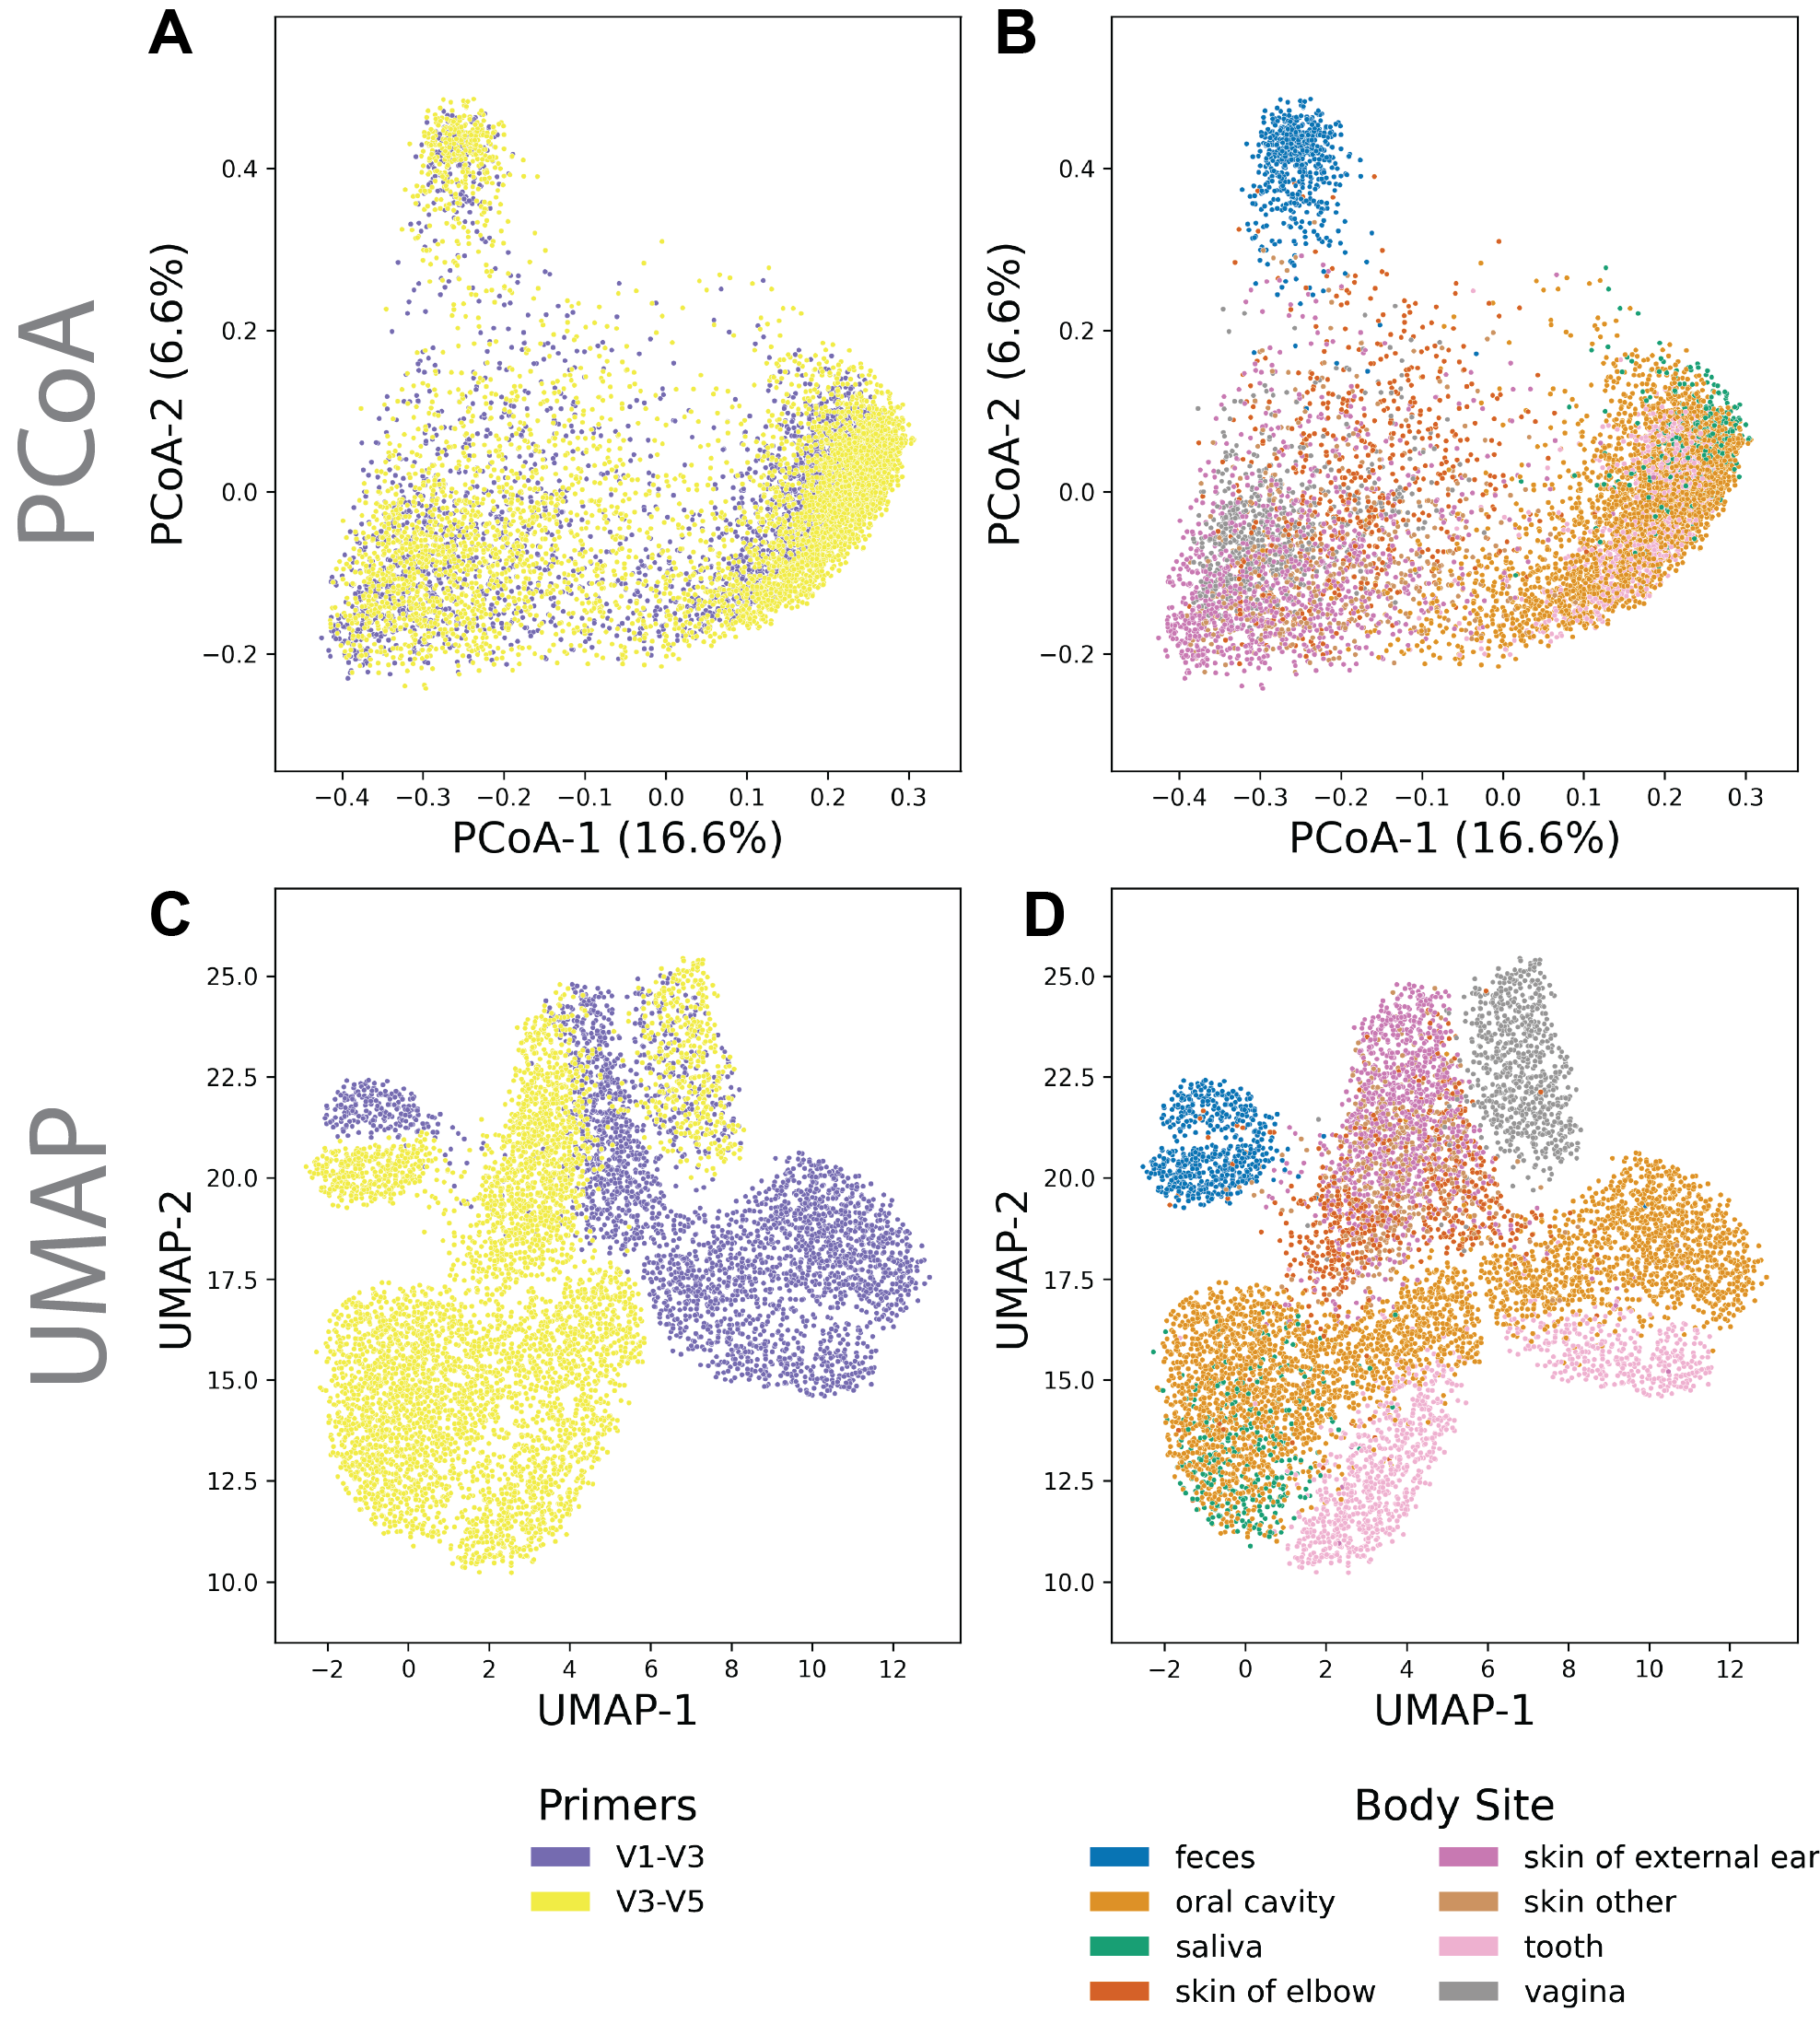
\includegraphics[width=\textwidth]{umap-figures/figure02.png}
\caption[PCoA and UMAP comparison on 8,280 samples from the Human Microbiome Project (HMP).]{\textbf{PCoA and UMAP comparison on 8,280 samples from the Human Microbiome Project (HMP).}  In the HMP data, when samples prepared with different primers are analyzed jointly, (A) there appears to be no separation between primers in the first two coordinates of PCoA and (B) mild separation by body site. In the same number of dimensions, UMAP is able to both (C) emphasize the differences between samples prepared with different variable regions and (D) improve clustering by body site. Both methods use the unweighted UniFrac distances on the HMP data rarefied to 1,000 sequences per sample.}
\label{umap_fig2}
\end{figure}

To quantify the clustering in the HMP data, we trained a k-Nearest Neighbors (kNN) classifier on the respective variables with 10-fold cross validation and reported the mean accuracy on the test folds. We trained kNN models on the first one, two, and three components of the PCoA, as well as fit UMAP embeddings for the respective number of dimensions. We found that kNN on a one-dimensional UMAP can outperform the sample site kNN for PCoA on up to 3 dimensions (Table~\ref{umap_table4}). kNN trained on a two-dimensional UMAP was able to distinguish primers more accurately than kNN on the first two principal coordinates. This indicates that UMAP is capable of representing multiple sources of variability in microbiome datasets with thousands of samples more distinctly and in fewer dimensions than PCoA.

\begin{table}[]
\caption{Comparison of 10-fold cross-validation accuracy of kNN in biological and technical variates}
\label{umap_table4}
\centering
\begin{tabular}{llll}
\hline \# of dimensions & Method & Target & Mean Accuracy \\ \hline
1 & PCoA & body\_habitat & 0.755556 \\
2 & PCoA & body\_habitat & 0.844203 \\
3 & PCoA & body\_habitat & 0.878140 \\
1 & UMAP Neighbors=8279 & body\_habitat & 0.924638 \\
1 & UMAP Neighbors=800 & body\_habitat & 0.929710 \\
2 & UMAP Neighbors=800 & body\_habitat & 0.932609 \\
2 & UMAP Neighbors=8279 & body\_habitat & 0.932850 \\
3 & UMAP Neighbors=800 & body\_habitat & 0.947222 \\
3 & UMAP Neighbors=8279 & body\_habitat & 0.947222 \\
1 & PCoA & qiita\_study\_id & 0.548913 \\
2 & PCoA & qiita\_study\_id & 0.570048 \\
1 & UMAP Neighbors=8279 & qiita\_study\_id & 0.805435 \\
1 & UMAP Neighbors=800 & qiita\_study\_id & 0.808937 \\
2 & UMAP Neighbors=8279 & qiita\_study\_id & 0.860990 \\
3 & PCoA & qiita\_study\_id & 0.891304 \\
2 & UMAP Neighbors=800 & qiita\_study\_id & 0.895773 \\
3 & UMAP Neighbors=800 & qiita\_study\_id & 0.916184 \\
3 & UMAP Neighbors=8279 & qiita\_study\_id & 0.916184 \\ \hline
\end{tabular}
\end{table}

	Finally, we explored a general-purpose recommendation for parameters. The parameters in this study were chosen to emphasize preserving the global structure of the data, by setting the `min\_dist' to its maximum of 1, increasing `n\_neighbors' from its default, and using default values for the rest of the parameters. In accordance with this goal, we set `n\_neighbors' to its maximum (n - 1 in general, 98 for soils, 87 for keyboard, and 8279 for the HMP) and re-ran the previous analyses. With this parameter setting, the results remain largely unchanged (Table~\ref{umap_table4}).
	Our benchmarks demonstrate the potential for improved performance and interpretability for both cluster and gradient microbiome data by using UMAP with its parameters set with the intent to preserve global geometry. Given that both algorithms provide different guarantees with respect to the preservation of distances in embeddings, we conclude that UMAP should be routinely used for microbiome analyses as a complement to PCoA. In order to facilitate using UMAP, we have made it conveniently available via QIIME2 \cite{Bolyen2019-fq} and Qiita \cite{Gonzalez2018-ez} plugins.
	
	
\section{Acknowledgements}

This work was supported in part by IBM Research AI through the AI Horizons Network, the Center for Microbiome Innovation at UC San Diego.

Chapter~\ref{chapter_umap}, in full, is a reprint of the material as it appears in ``Uniform Manifold Approximation and Projection (UMAP) Reveals Composite Patterns and Resolves Visualization Artifacts in Microbiome Data.'' George Armstrong, Cameron Martino, Gibraan Rahman, Antonio Gonzalez, Yoshiki Vázquez-Baeza, Gal Mishne, and Rob Knight.  \textit{mSystems 6}, 2021. The dissertation author was the primary investigator and the first author of this paper.


\chapter{Swapping metagenomics preprocessing pipeline components offers speed and sensitivity increases}\label{chapter_host_filtering}


\glsresetall

% \section{Abstract}

Increasing data volumes on high-throughput sequencing instruments such as the NovaSeq 6000 leads to long computational bottlenecks for common metagenomics data preprocessing tasks such as adaptor and primer trimming and host removal. Here we test whether faster recently developed computational tools (Fastp and Minimap2) can replace widely used choices (Atropos and Bowtie2), obtaining dramatic accelerations with additional sensitivity and minimal loss of specificity for these tasks. Furthermore, the taxonomic tables resulting from downstream processing provide biologically comparable results. However, we demonstrate that for taxonomic assignment, Bowtie2’s specificity is still required. We suggest that periodic re-evaluation of pipeline components, together with improvements to standardized APIs to chain them together, will greatly enhance the efficiency of common bioinformatics tasks while also facilitating incorporation of further optimized steps running on GPUs, FPGAs, or other architectures. We also note that a detailed exploration of available algorithms and pipeline components is an important step that should be taken before optimization of less efficient algorithms on advanced or non-standard hardware.

\section{Importance}
In shotgun metagenomics studies that seek to relate changes in microbial DNA across samples, processing the data on a computer often takes longer than obtaining the data from the sequencing instrument. Recently developed software packages that perform individual steps in the pipeline of data processing in principle offer speed advantages, but in practice may contain pitfalls that prevent their use, for example, they may make approximations that introduce unacceptable errors in the data. Here we show that differences in choices of these components can speed up overall data processing by 5-fold or more on the same hardware while maintaining a high degree of correctness, greatly reducing the time taken to interpret results. This is an important step for using the data in clinical settings, where the time taken to obtain the results may be critical for guiding treatment. 

\section{Observation}

The universal first step in processing metagenomic and metatranscriptomic data is quality filtering and trimming (i.e. removing low-quality reads and removing sequences introduced as technical artifacts such as sequencing adaptors and PCR primers), so that only high-quality data that corresponds to nucleic acid sequences in the original samples is retained. For samples derived from humans, or where host DNA dominates over microbial DNA (for example, biopsy specimens, surface swabs from skin or plants, etc.), filtering out sequences that are derived from the host rather than microbes is also important for ethical and/or technical reasons. Increasing data volumes with newer sequencing instrumentation have transformed these steps from minor nuisances to efforts that require major computation, typically involving clusters or cloud computing solutions.

A widely used combination for quality filtering, trimming and host filtering is Atropos \cite{Didion2017-pl} plus Bowtie2 \cite{Langmead2012-lz}, both of which are popular and widely used tools for these tasks. A few of the many examples of publications that have used either tool for these tasks include comparisons of multiple pipelines for nucleic acid extraction \cite{Shaffer2021-mf}, analysis of a large Finnish cardiac risk cohort \cite{Salosensaari2021-qf}, the popular KneadData preprocessing tool \cite{McIver2018-rk} and a recent paper examining the metavirome of the mosquito Aedes aegypti \cite{Ramos-Nino2020-tr}. 

As datasets have scaled rapidly, the need for near-real-time processing to support clinical applications such as choice of antibiotics in sepsis, determination of respiratory symptoms as bacterial or viral (including novel pathogens such as SARS-CoV-2), and choice of anti-cancer medications have prompted exploration of hardware acceleration approaches such as GPUs  \cite{Sandes2016-tj}, FPGAs \cite{Shah2013-ot}, and in-memory computing approaches \cite{Gupta2019-sd} for key analysis steps, including alignment. Driven by weeks- to months-long delays in processing data from large projects, in the DARPA-sponsored JUMP-CRISP project, we sought to benchmark and characterize the slow steps in the popular Atropos plus Bowtie2 pipeline. However, prior to proceeding directly to implementation of this pipeline on an alternative architecture, we sought to determine whether other CPU-based tools might provide sufficient performance improvement and/or provide a better candidate for acceleration.

Here we explored other combinations of popular methods, and found that the combination of Fastp \cite{Chen2018-zx} (trimming) and Minimap2 \cite{Li2018-bw} (host-filtering) performed best. We then demonstrated that this faster combination of processing produces outputs that are quantitatively similar to previous conventional methods in both data-driven simulation data and real data derived from a broad set of extraction kits and sample types.

While implementing the host-filtering benchmarks, we discovered a read count limitation with Bowtie2. When used on large sequencing data sets, the reads after 232 were not included in Bowtie2's output, prohibiting successful application of host-filtering on full NovaSeq lanes. We subsequently fixed this and the update is available in Bowtie2 v2.4.2 or later (see \href{https://github.com/BenLangmead/bowtie2/pull/312}{here}). We used this updated version in our benchmarks.

To evaluate runtime performance, we used the popular CAMI-Sim package \cite{Fritz2019-vg}, one of the important outputs of the CAMI (Critical Assessment of Metagenome Interpretation) project \cite{Sczyrba2017-wx}, to generate simulated datasets containing known amounts of host genome contamination. The simulated data contained 150 bp reads sampled from 10 microbial and 1 human reference genome (Table~\ref{host_filtering_table_S1}). Errors were simulated into the reads with ART \cite{Huang2012-nl} using Illumina default error profiles. Minimap2 (preset for short-reads), Bowtie2 (which allows several preset modes that trade-off sensitivity for speed) and BWA MEM \cite{Li2013-xz} (no presets, so defaults were used) were run with 12 threads to align the simulated reads to a different human reference (T2T CHM13).  Figure~\ref{host_filtering_fig1} documents the reduction in read misclassification (Figure~\ref{host_filtering_fig1}A) and false negatives (Figure~\ref{host_filtering_fig1}B) of host-filtering by Minimap2 and BWA MEM over Bowtie2. Minimap2 provides a 1.6-8.3-fold improvement in speed of computation on the same data, compared to the most sensitive version of Bowtie2, while offering 10.5-44.3-fold improvement over BWA (Figure~\ref{host_filtering_fig1}C). Compared to Bowtie2, Minimap2’s runtime performs more favorably with the amount of host contamination, making it suitable for even highly host contaminated samples such as tissue biopsies, saliva, nasal cavity, skin, and vaginal samples, which can contain \>90\% host DNA \cite{Poore2020-yh,Marotz2018-yq}. It is also notable that while the rate Bowtie2 and BWA MEM process reads at a relatively constant rate across all the tested read counts, Minimap2 does not achieve optimal performance until it operates on a larger number of reads (Figure~\ref{host_filtering_fig1}D). For runtime, we have focused on the host filtering step because it took the bulk of the time, and the results of trimming are largely unchanged between Fastp and Atropos (Figure~\ref{host_filtering_figS1}A).   When comparing the widely-used combination of Atropos plus Bowtie2 to the new fastest approach of Fastp plus Minimap2, we note that the overall pipeline, including trimming and filtering components, was accelerated overall by a factor of 5.6 (Figure~\ref{host_filtering_figS1}B), which may come at the cost of increased memory usage (Figure~\ref{host_filtering_figS1}C).

\begin{figure}[htbp]
\centering
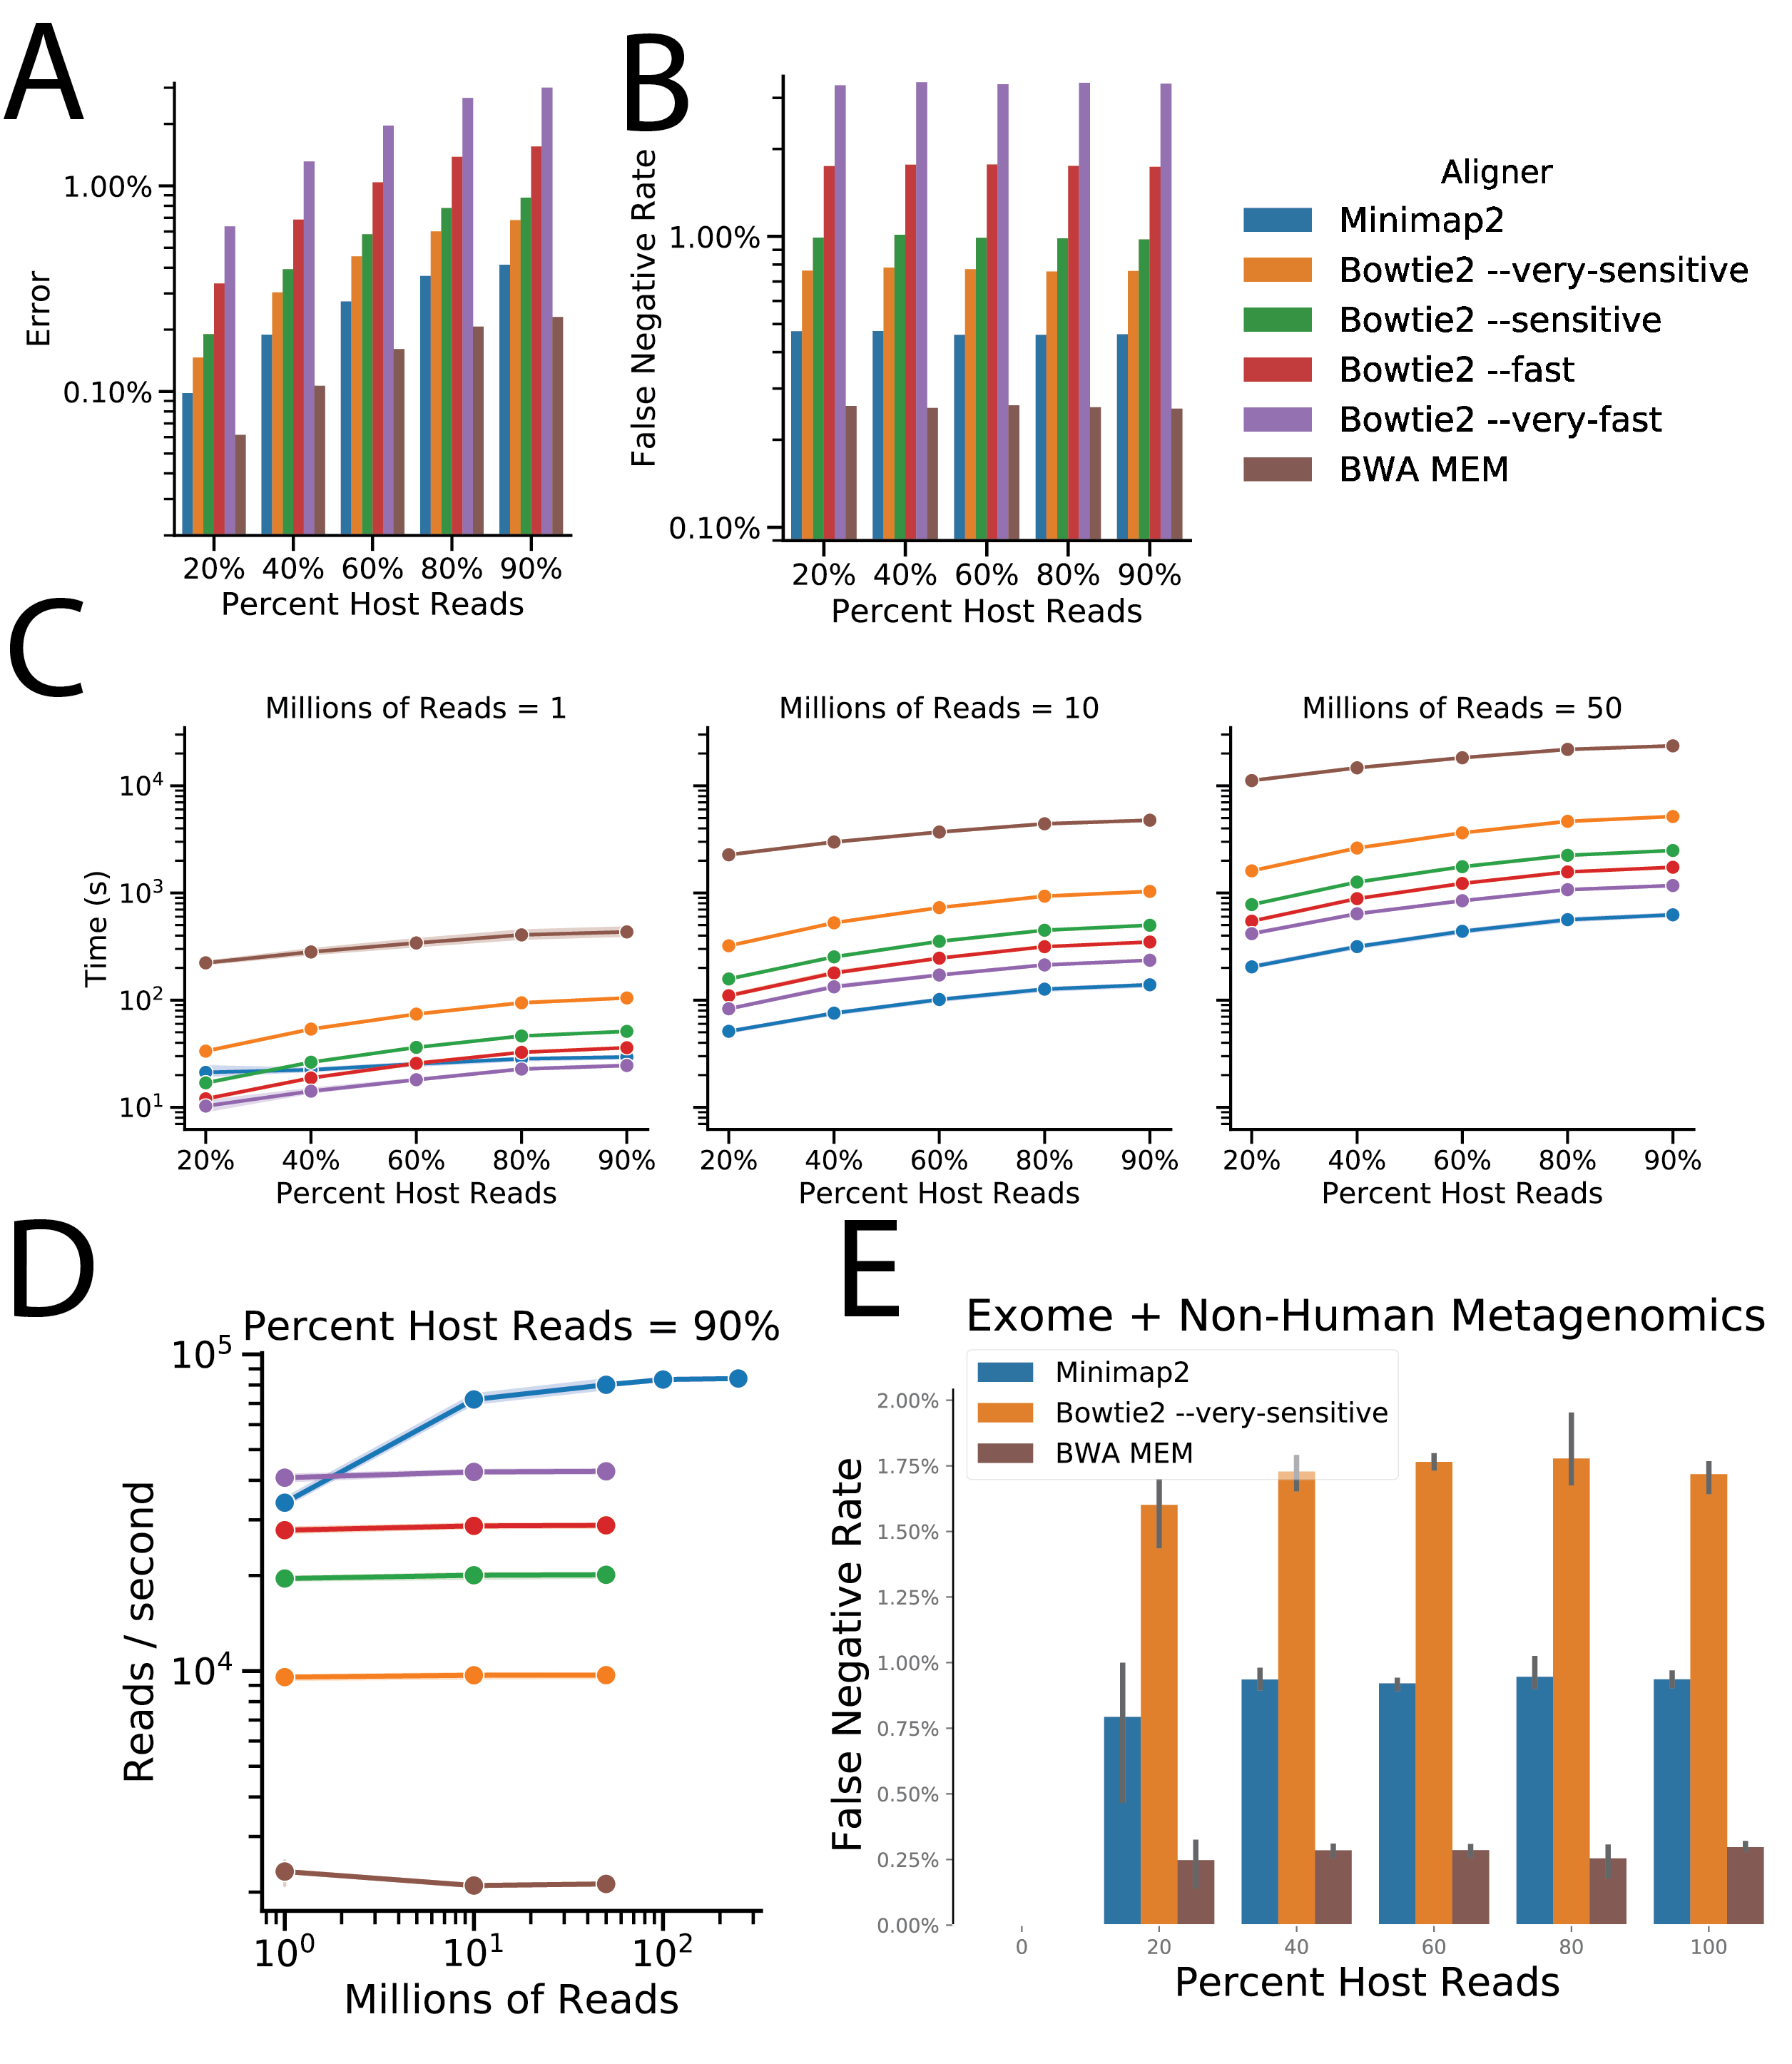
\includegraphics[width=0.95\textwidth]{host-filtering-figures/figure01.png}
\caption[Minimap2 provides improved error, sensitivity, and runtime for host-filtering over the current open-source pipeline.]{\textbf{Minimap2 provides improved error, sensitivity, and runtime for host-filtering over the current open-source pipeline.} Comparison of aligners for host-filtering on 1 million CAMI-sim simulated reads by (A) error and (B) human reads failed to align to the reference (false negative rate). (C) Time and (D) processing rate comparison across aligners of 1 million, 10 million, and 50 million CAMI-sim simulated reads. Minimap2 is shown for 100 million and 250 million reads. (E) False negative rate of host filtering on data with real reads combined from separate exome sequencing and non-human metagenomics studies.}
\label{host_filtering_fig1}
\end{figure}

In order to further validate the results between Bowtie2, BWA MEM, and Minimap2 on real sequencing data, we created in silico mock mixtures of data from known sources.  We first obtained IGSR phase 3 \cite{Clarke2017-qi} human exome sequencing data (Table~\ref{host_filtering_table_S1}) that is likely to be free of microbial genomic contamination compared to whole-genome sequencing, which can be contaminated with microbial reads \cite{Poore2020-yh}.  Then, we obtained soil rhizosphere and mouse fecal metagenomics sequencing data, free of any human genome contamination. From these two datasets we produced benchmarking samples of 1 thousand, 100 thousand, and 1 million total sequences with varying proportions of microbial vs. human derived sequencing data ranging from 0-100\% human. The samples were then processed by Bowtie2 (very-sensitive), BWA MEM, and Minimap2. As observed in the simulation data, in all conditions Minimap2 and BWA MEM outperformed the most sensitive version of Bowtie2 in allowing fewer human sequences to pass read filtering (Figure~\ref{host_filtering_fig1}E).

Although these results on simulated data were encouraging, it is critical to benchmark new techniques on real-world data. We therefore used one of our recently published datasets comparing different nucleic acid extraction methods, which provided a built-in way of comparing for any differences of biological interpretation between the previously established end-to-end pipeline and the new, fastest combination of Fastp and Minimap2. These kit comparisons datasets contain samples from  a range of biospecimen types with differing host DNA load \cite{Shaffer2021-mf}. Across the three extraction conditions tested in that paper, the total number of reads recovered from each sample was essentially identical between the Atropos/Bowtie2 and the Fastp/Minimap2 pipelines (Figure~\ref{host_filtering_fig2}A), and the alpha diversity estimates within each sample were also essentially identical (Figure~\ref{host_filtering_fig2}B). The sample pairs with different host-filtering methods were also extremely similar in unweighted and weighted ordination results (Figure~\ref{host_filtering_fig2}C), with differences between individual specimens run through both pipelines (connected by lines) typically much smaller than differences between different specimens, even of the same biospecimen types. Finally, the overlap of taxonomic calls at the phylum, genus and species level was perfect between the two pipelines (Figure~\ref{host_filtering_fig2}D).

\begin{figure}[htbp]
\centering
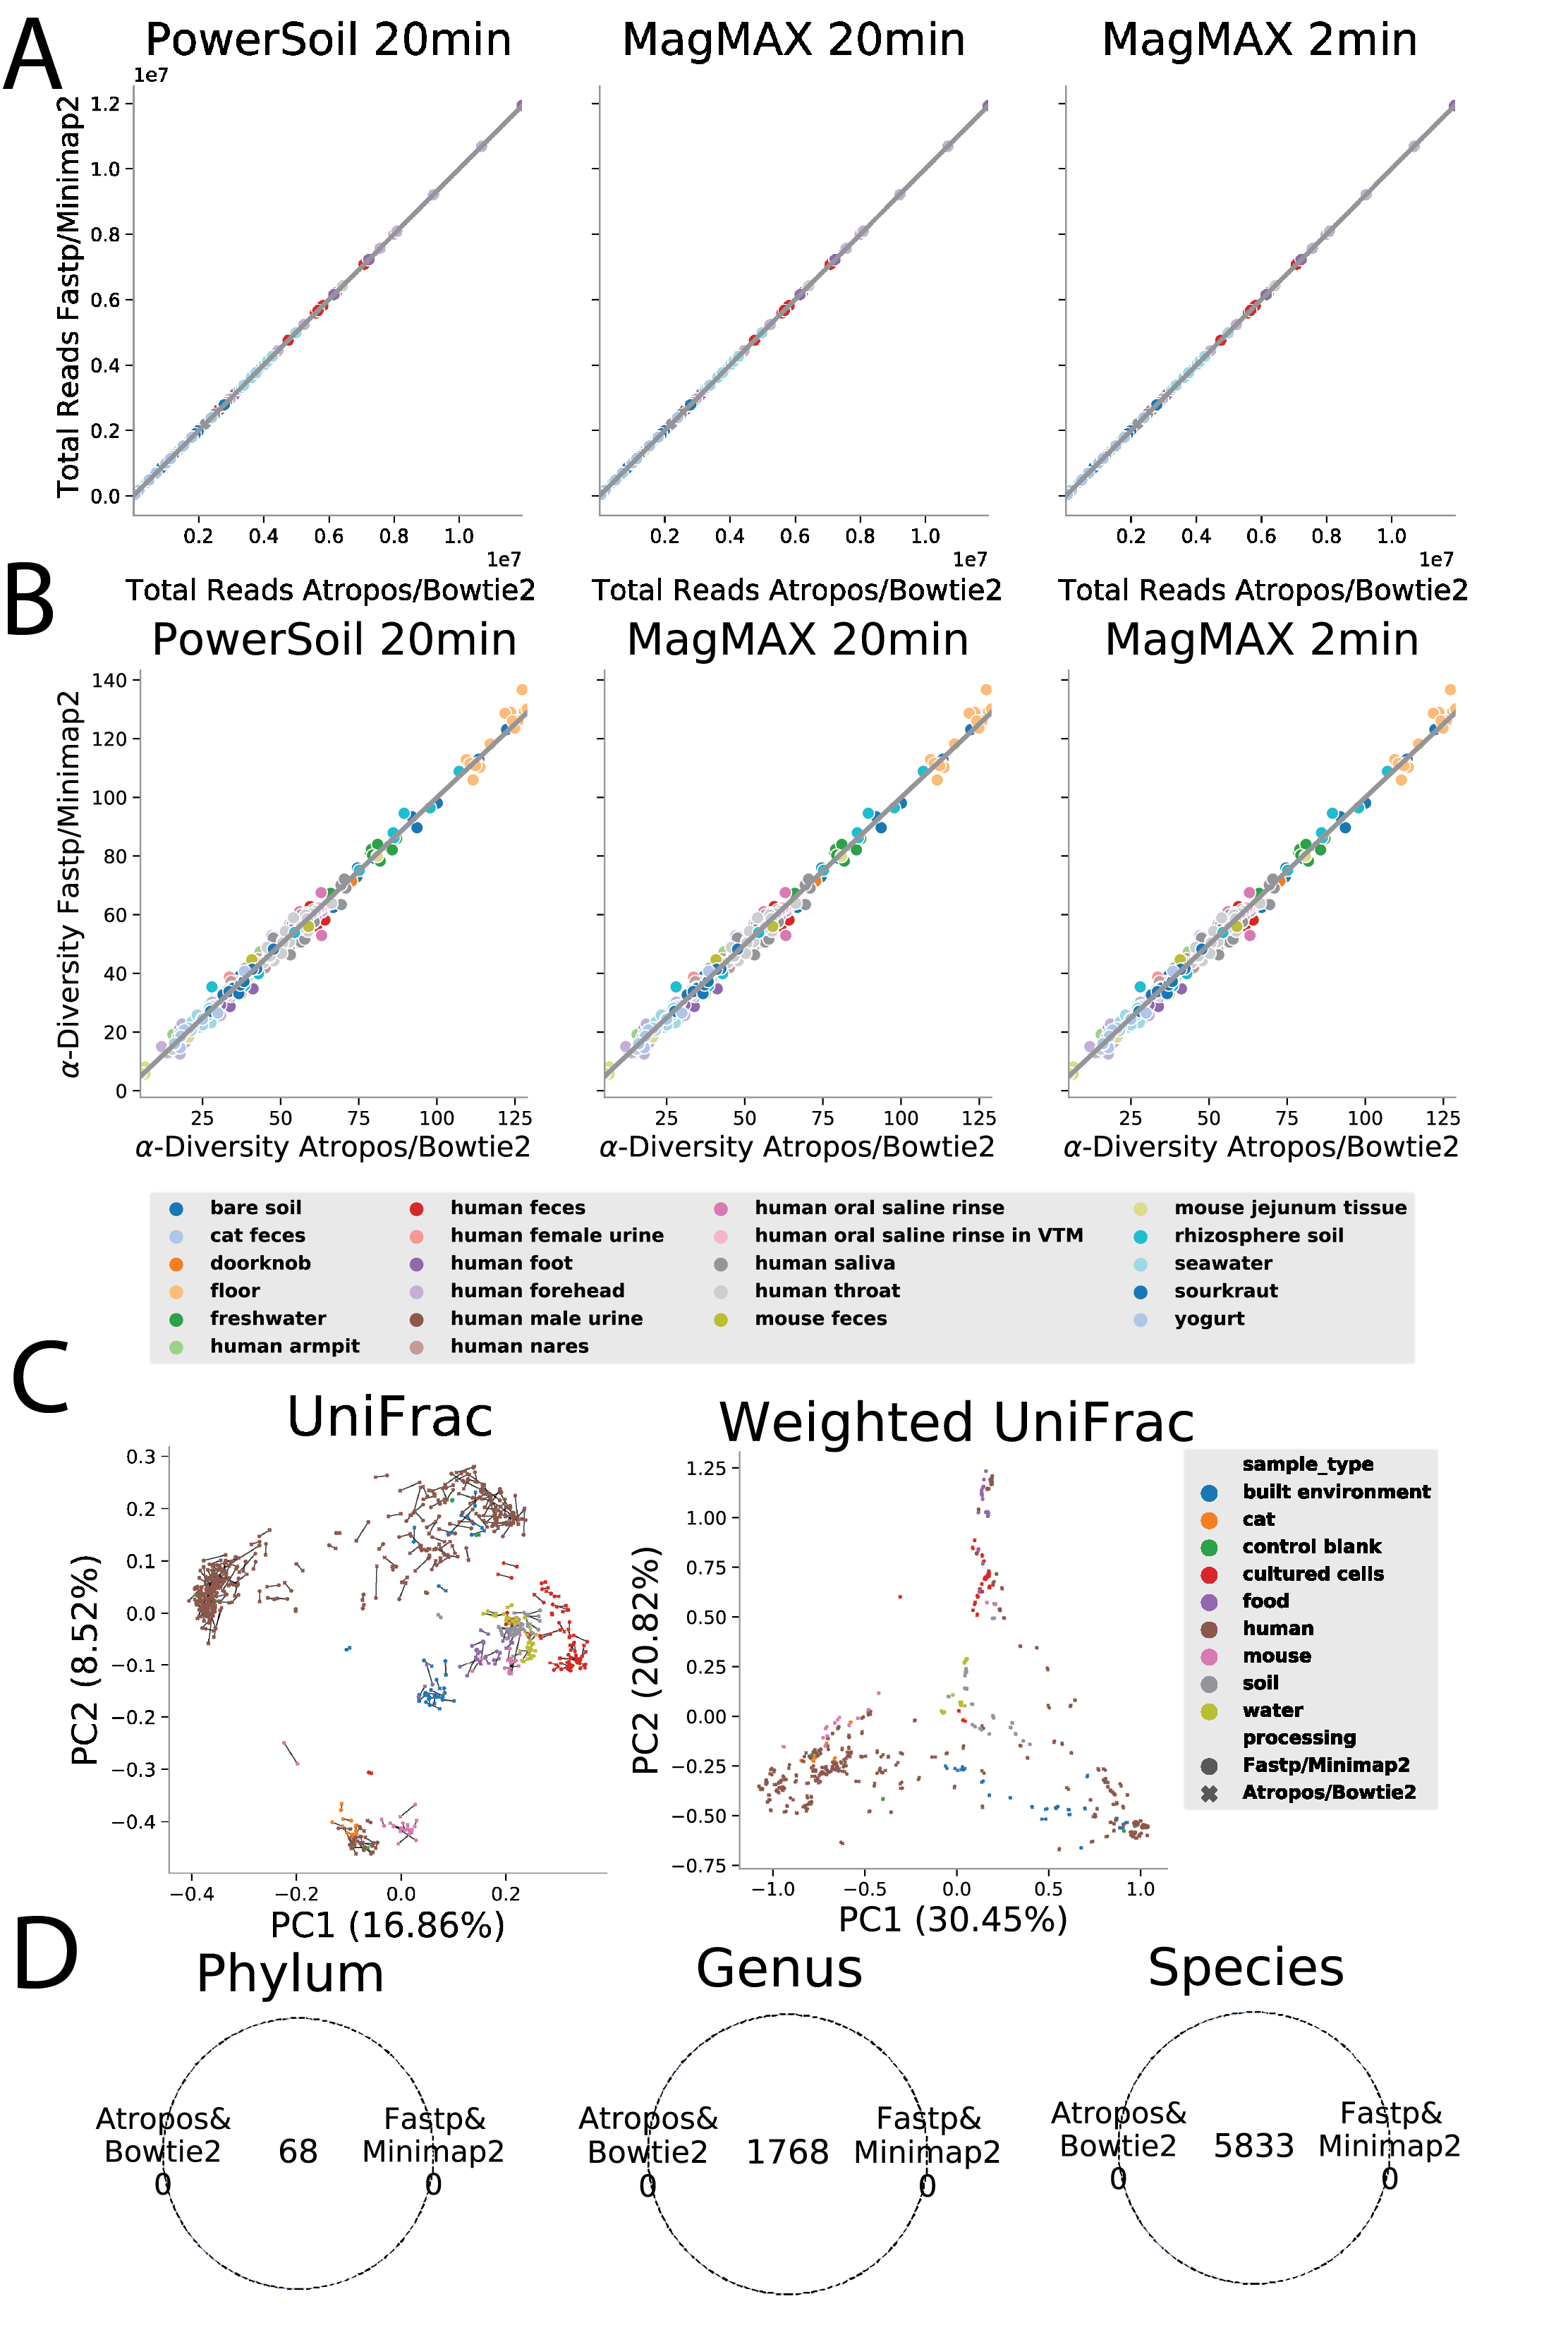
\includegraphics[width=0.7\textwidth]{host-filtering-figures/figure02.png}
\caption[When comparing broad sets of extraction kits and sample types, Minimap2/Fastp processing results do not differ in biological interpretation compared to current processing methods.]{\textbf{When comparing broad sets of extraction kits and sample types, Minimap2/Fastp processing results do not differ in biological interpretation compared to current processing methods.}  (A and B) Comparison of total reads passing the filter (A) and Faith's phylogenetic diversity (B) for Fastp/Minimap2 (y axes) and Atropos/Bowtie2 (x axes) colored by sample type. (C) Principal coordinate analysis (PCoA) on unweighted (left) and weighted (right) UniFrac compared between Fastp/Minimap2 (circles) and Atropos/Bowtie2 (cross) colored by sample source environment. (D) Comparison of shared features between processing methods fastp/Minimap2 and Atropos/Bowtie2 at the phylum, genus, and species taxonomic levels.}
\label{host_filtering_fig2}
\end{figure}

Given the dramatic improvement in preprocessing and host filtering, we further sought to test whether Minimap2 is suitable for taxonomic assignment with similar speed advantages, compared to Bowtie2, which is used in the Woltka pipeline \cite{Zhu2021-ap}. Using Woltka benchmarking datasets for taxonomic assignment, we found Minimap2 performs  comparatively poorly, with a reduced F1-score (Figure~\ref{host_filtering_figS2}A). This is potentially attributed to the higher false positive rate of Minimap2 (Figure~\ref{host_filtering_figS2}B), since it will result in more alternate alignments between similar genomes, which detract Woltka's accuracy. Research into accelerating this part of the overall analysis pipeline for shotgun metagenomics data should therefore focus on accelerating other methods, rather than Minimap2.

Taken together, our results suggest several important principles for optimization of shotgun metagenomics workflows. First, even widely used pipeline components should be periodically re-evaluated to test whether more efficient implementations or better algorithms are available and can be substituted with substantial speed improvements. This benchmarking is facilitated by standardized options and interfaces, and standardized datasets, and we make the datasets we produced here available for reuse. Second, before investing substantial effort in developing nonstandard hardware or approaches to accelerate a specific algorithm, it is worth checking whether a better CPU-based algorithm is available, and then, if it is, optimizing that other algorithm instead. Finally, caution is warranted in generalizing which pipeline steps a given algorithm or implementation is used for. Although Minimap2 and Bowtie2 both fundamentally perform the same task (approximate string match to a database, albeit with different mechanisms), Minimap2’s failure on the taxonomic assignment task warrants further investigation to test whether the algorithm could be adapted to this task or whether there are fundamental limitations.


Our current work therefore provides an important practical improvement with a speedup in common metagenomics preprocessing tasks, which we have already made available to the community via incorporation into Qiita \cite{Gonzalez2018-ez}. Future work will be needed to assess and adapt alignment-free approaches, which often provide improvements in runtime over alignment methods, for both host-filtering and taxonomic assignment tasks. These advancements also point the way towards further optimization that will allow real-time or near-real-time use of metagenomic and/or metatranscriptomic data in clinical decision making, where time is often of the essence.

\section{Acknowledgements}
This work was supported in part by CRISP, one of six centers in JUMP, a Semiconductor Research Corporation (SRC) program sponsored by DARPA. \\ https://crisp.engineering.virginia.edu/. J.P.S. was supported by NIH/NIGMS IRACDA K12 GM068524.

Chapter~\ref{chapter_host_filtering}, in full, is a reprint of the material as it appears in ``Swapping metagenomics preprocessing pipeline components offers speed and sensitivity increases.'' George Armstrong, Cameron Martino, Justin Morris, Behnam Khaleghi, Jaeyoung Kang, Jeff DeReus, Qiyun Zhu, Daniel Roush, Daniel McDonald, Antonio Gonzalez, Justin Shaffer, Carolina Carpenter, Mehrbod Estaki, Stephen Wandro, Sean Eilert, Ameen Akel, Justin Eno, Ken Curewitz, Austin D. Swafford, Niema Moshiri, Tajana Rosing, and Rob Knight. \textit{mSystems e0137821}, 2022. The dissertation author was a primary investigator and co-first author of this paper.


\appendix
\chapter{Supplemental Material for 
Chapter~\ref{chapter_umap}}

\begin{figure}[htbp]
\centering
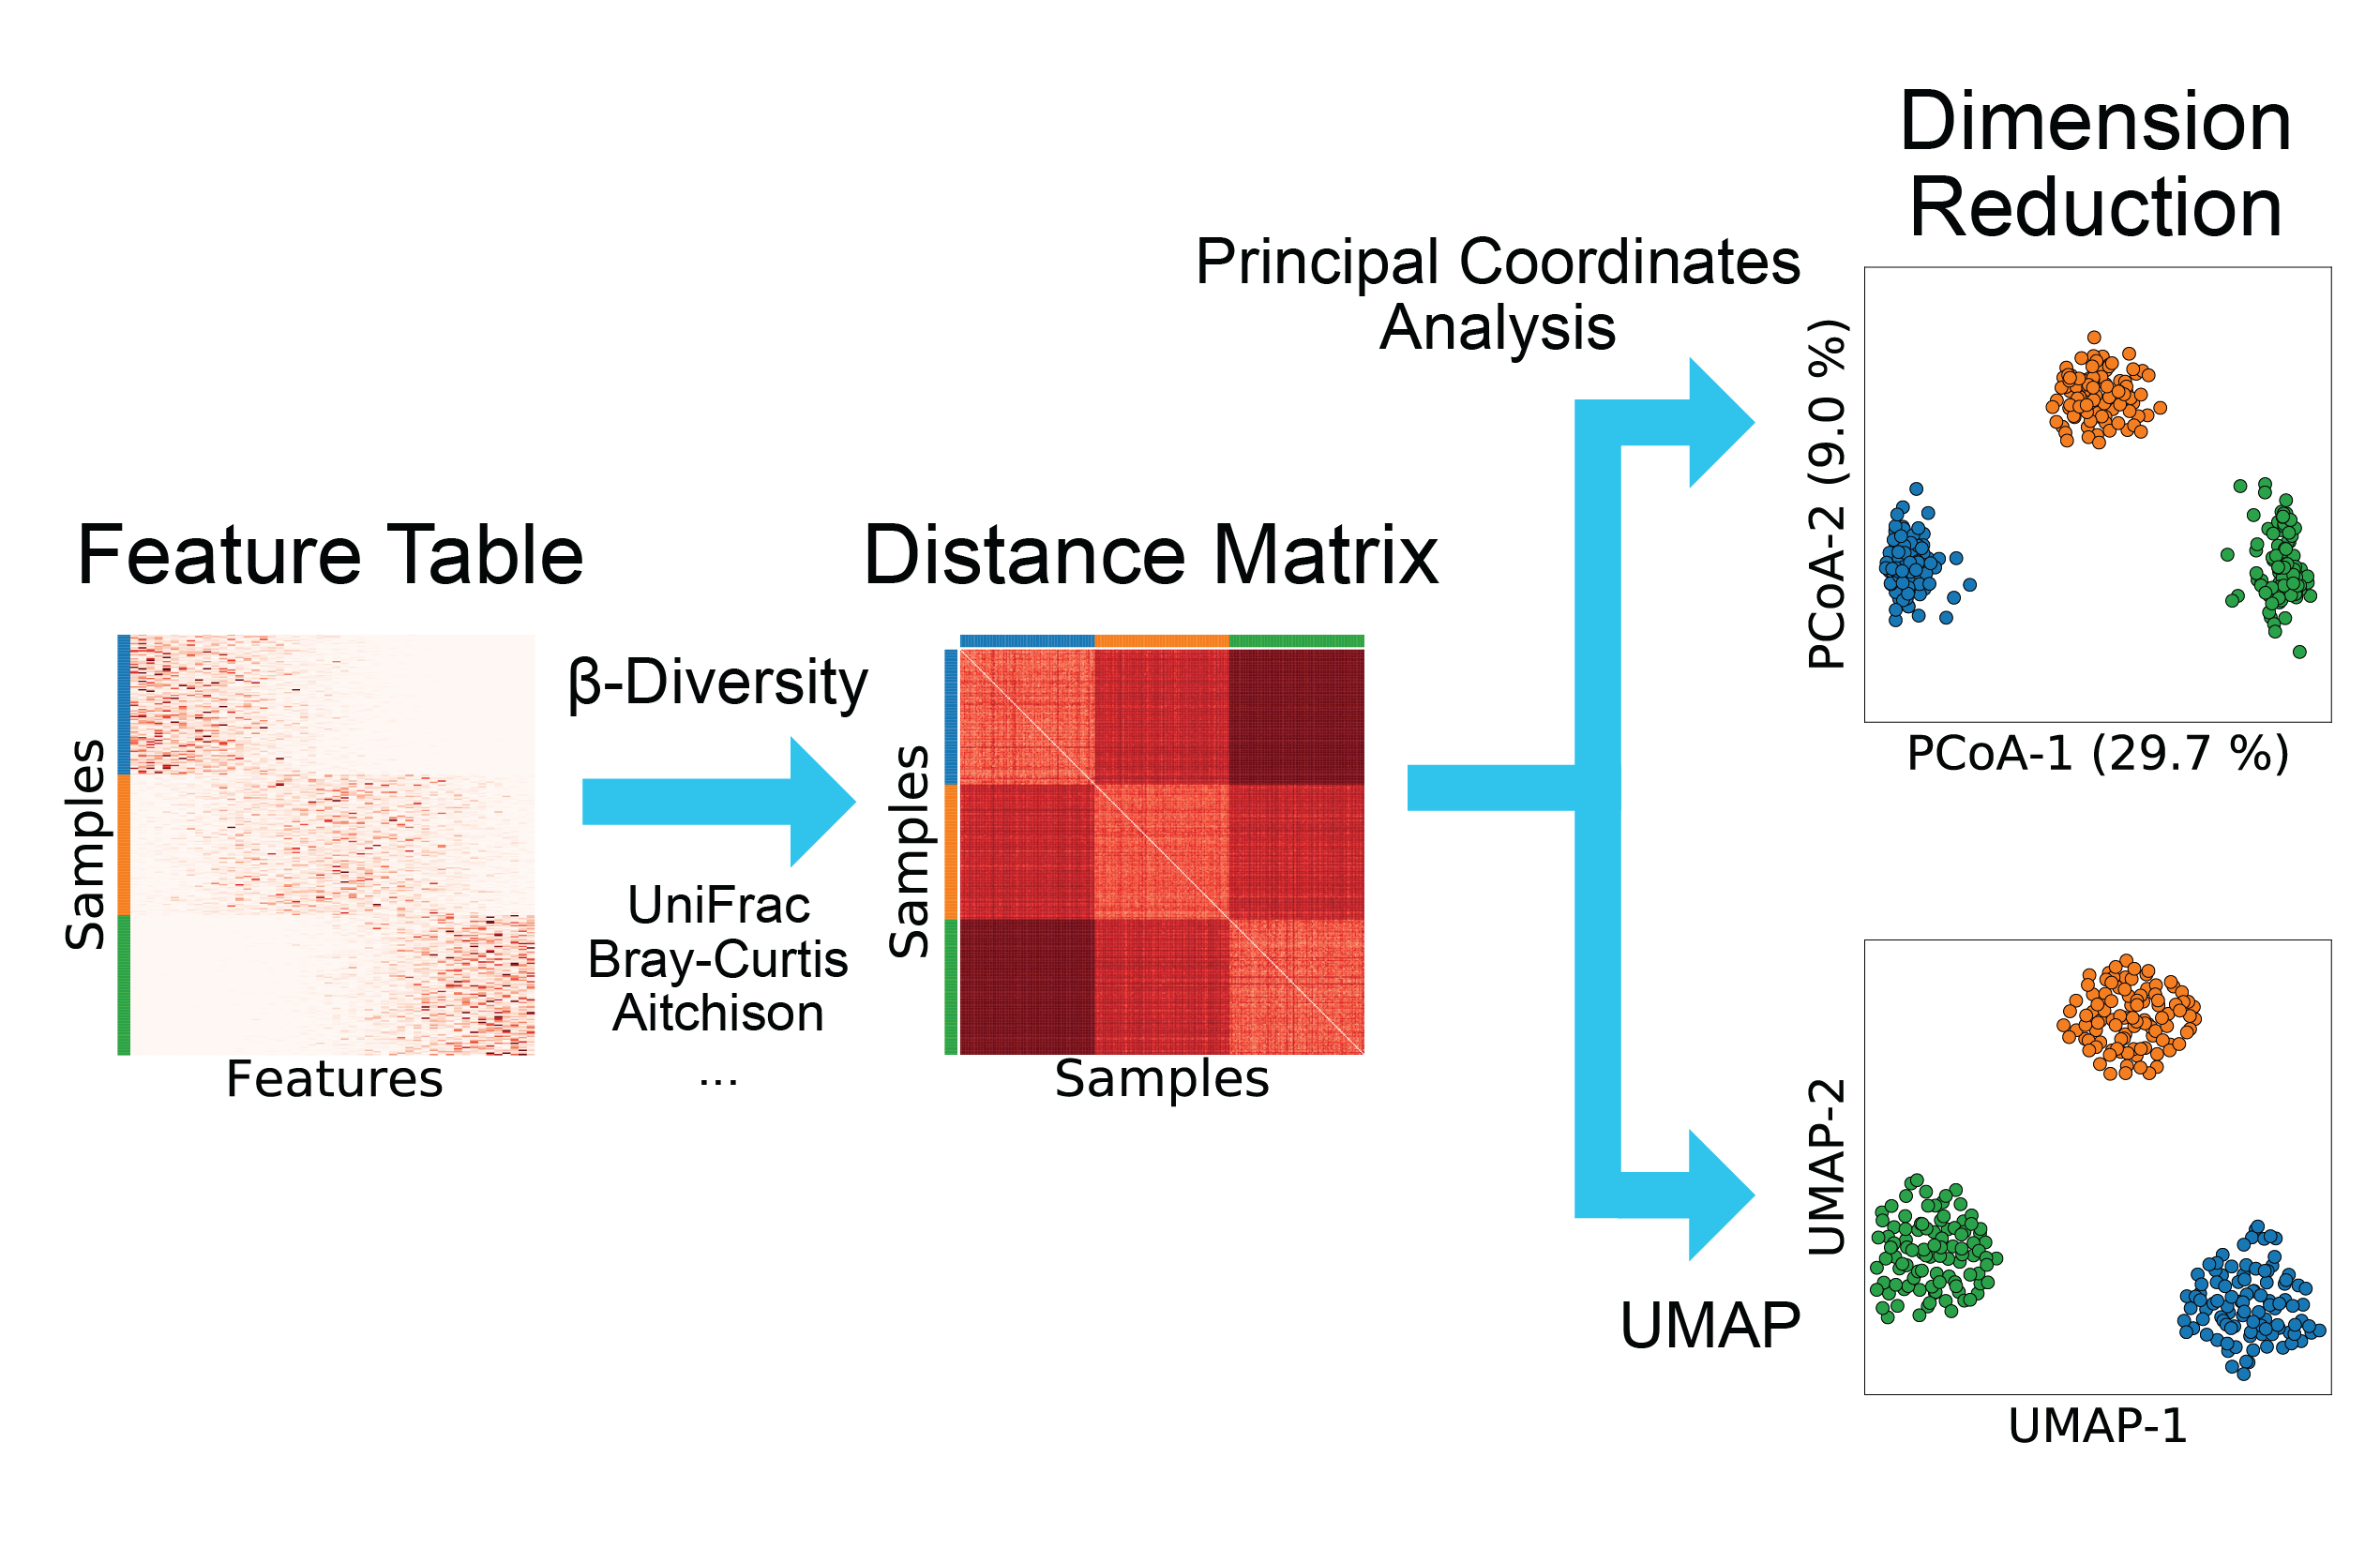
\includegraphics[width=\textwidth]{umap-figures/figureS01.png}
\caption[Graphical abstract.]{\textbf{Graphical abstract.} UMAP can operate on distance matrices of arbitrary distance metrics (UniFrac, Bray-Curtis, Aitchison), similarly to PCoA.}
\label{umap_figS1}
\end{figure}

\begin{figure}[htbp]
\centering
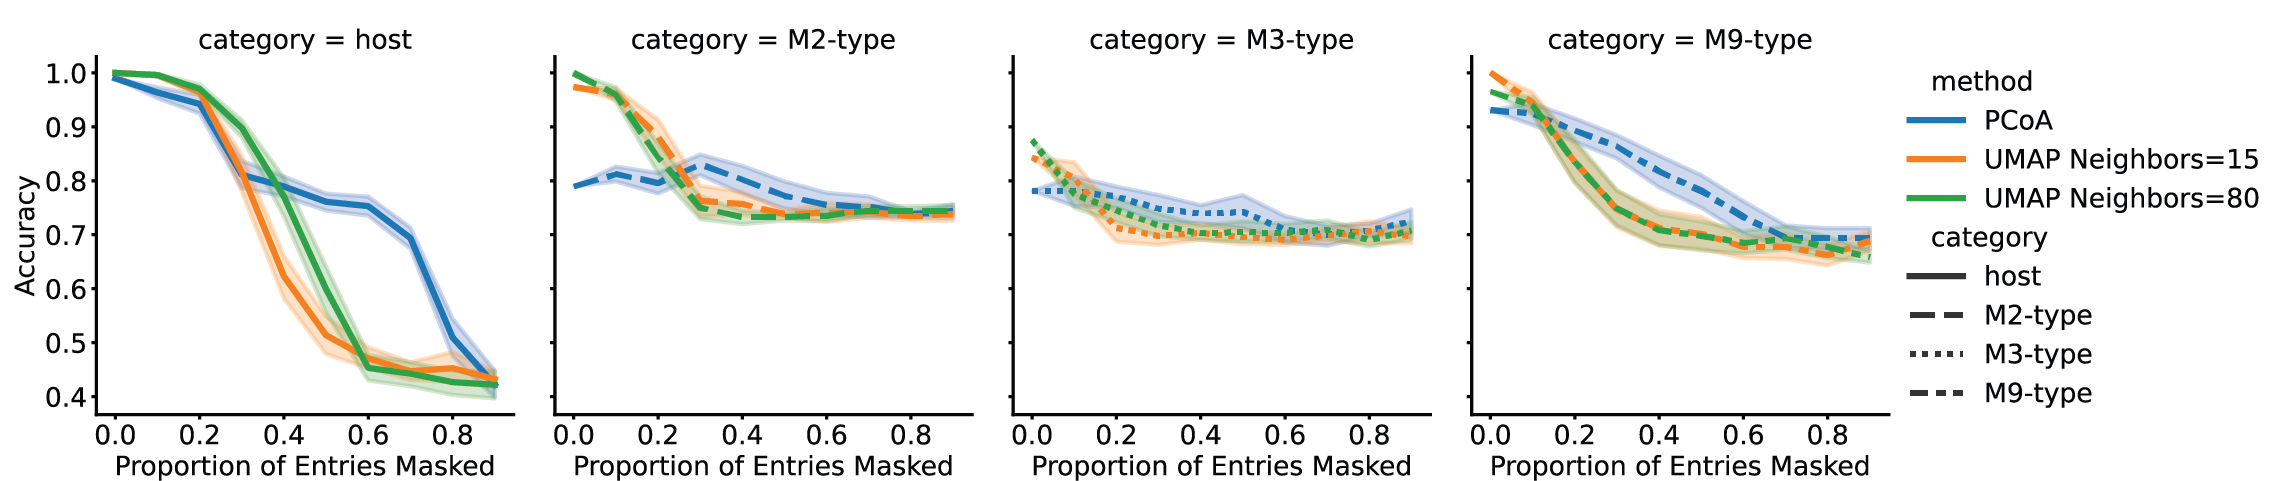
\includegraphics[width=\textwidth]{umap-figures/figureS02.png}
\caption[Simulated missing data on keyboard study.]{\textbf{Simulated missing data on keyboard study.} A proportion of the entries of the table were randomly masked (20 repetitions per ablation level) from the feature table, and dimensionality reduction followed by LDA was run on each of the tables. Host accuracy is the accuracy for identifying the correct subject. The subject-type accuracies are specific sample-type accuracies specific to the individual.}
\label{umap_figS2}
\end{figure}

\begin{figure}[htbp]
\centering
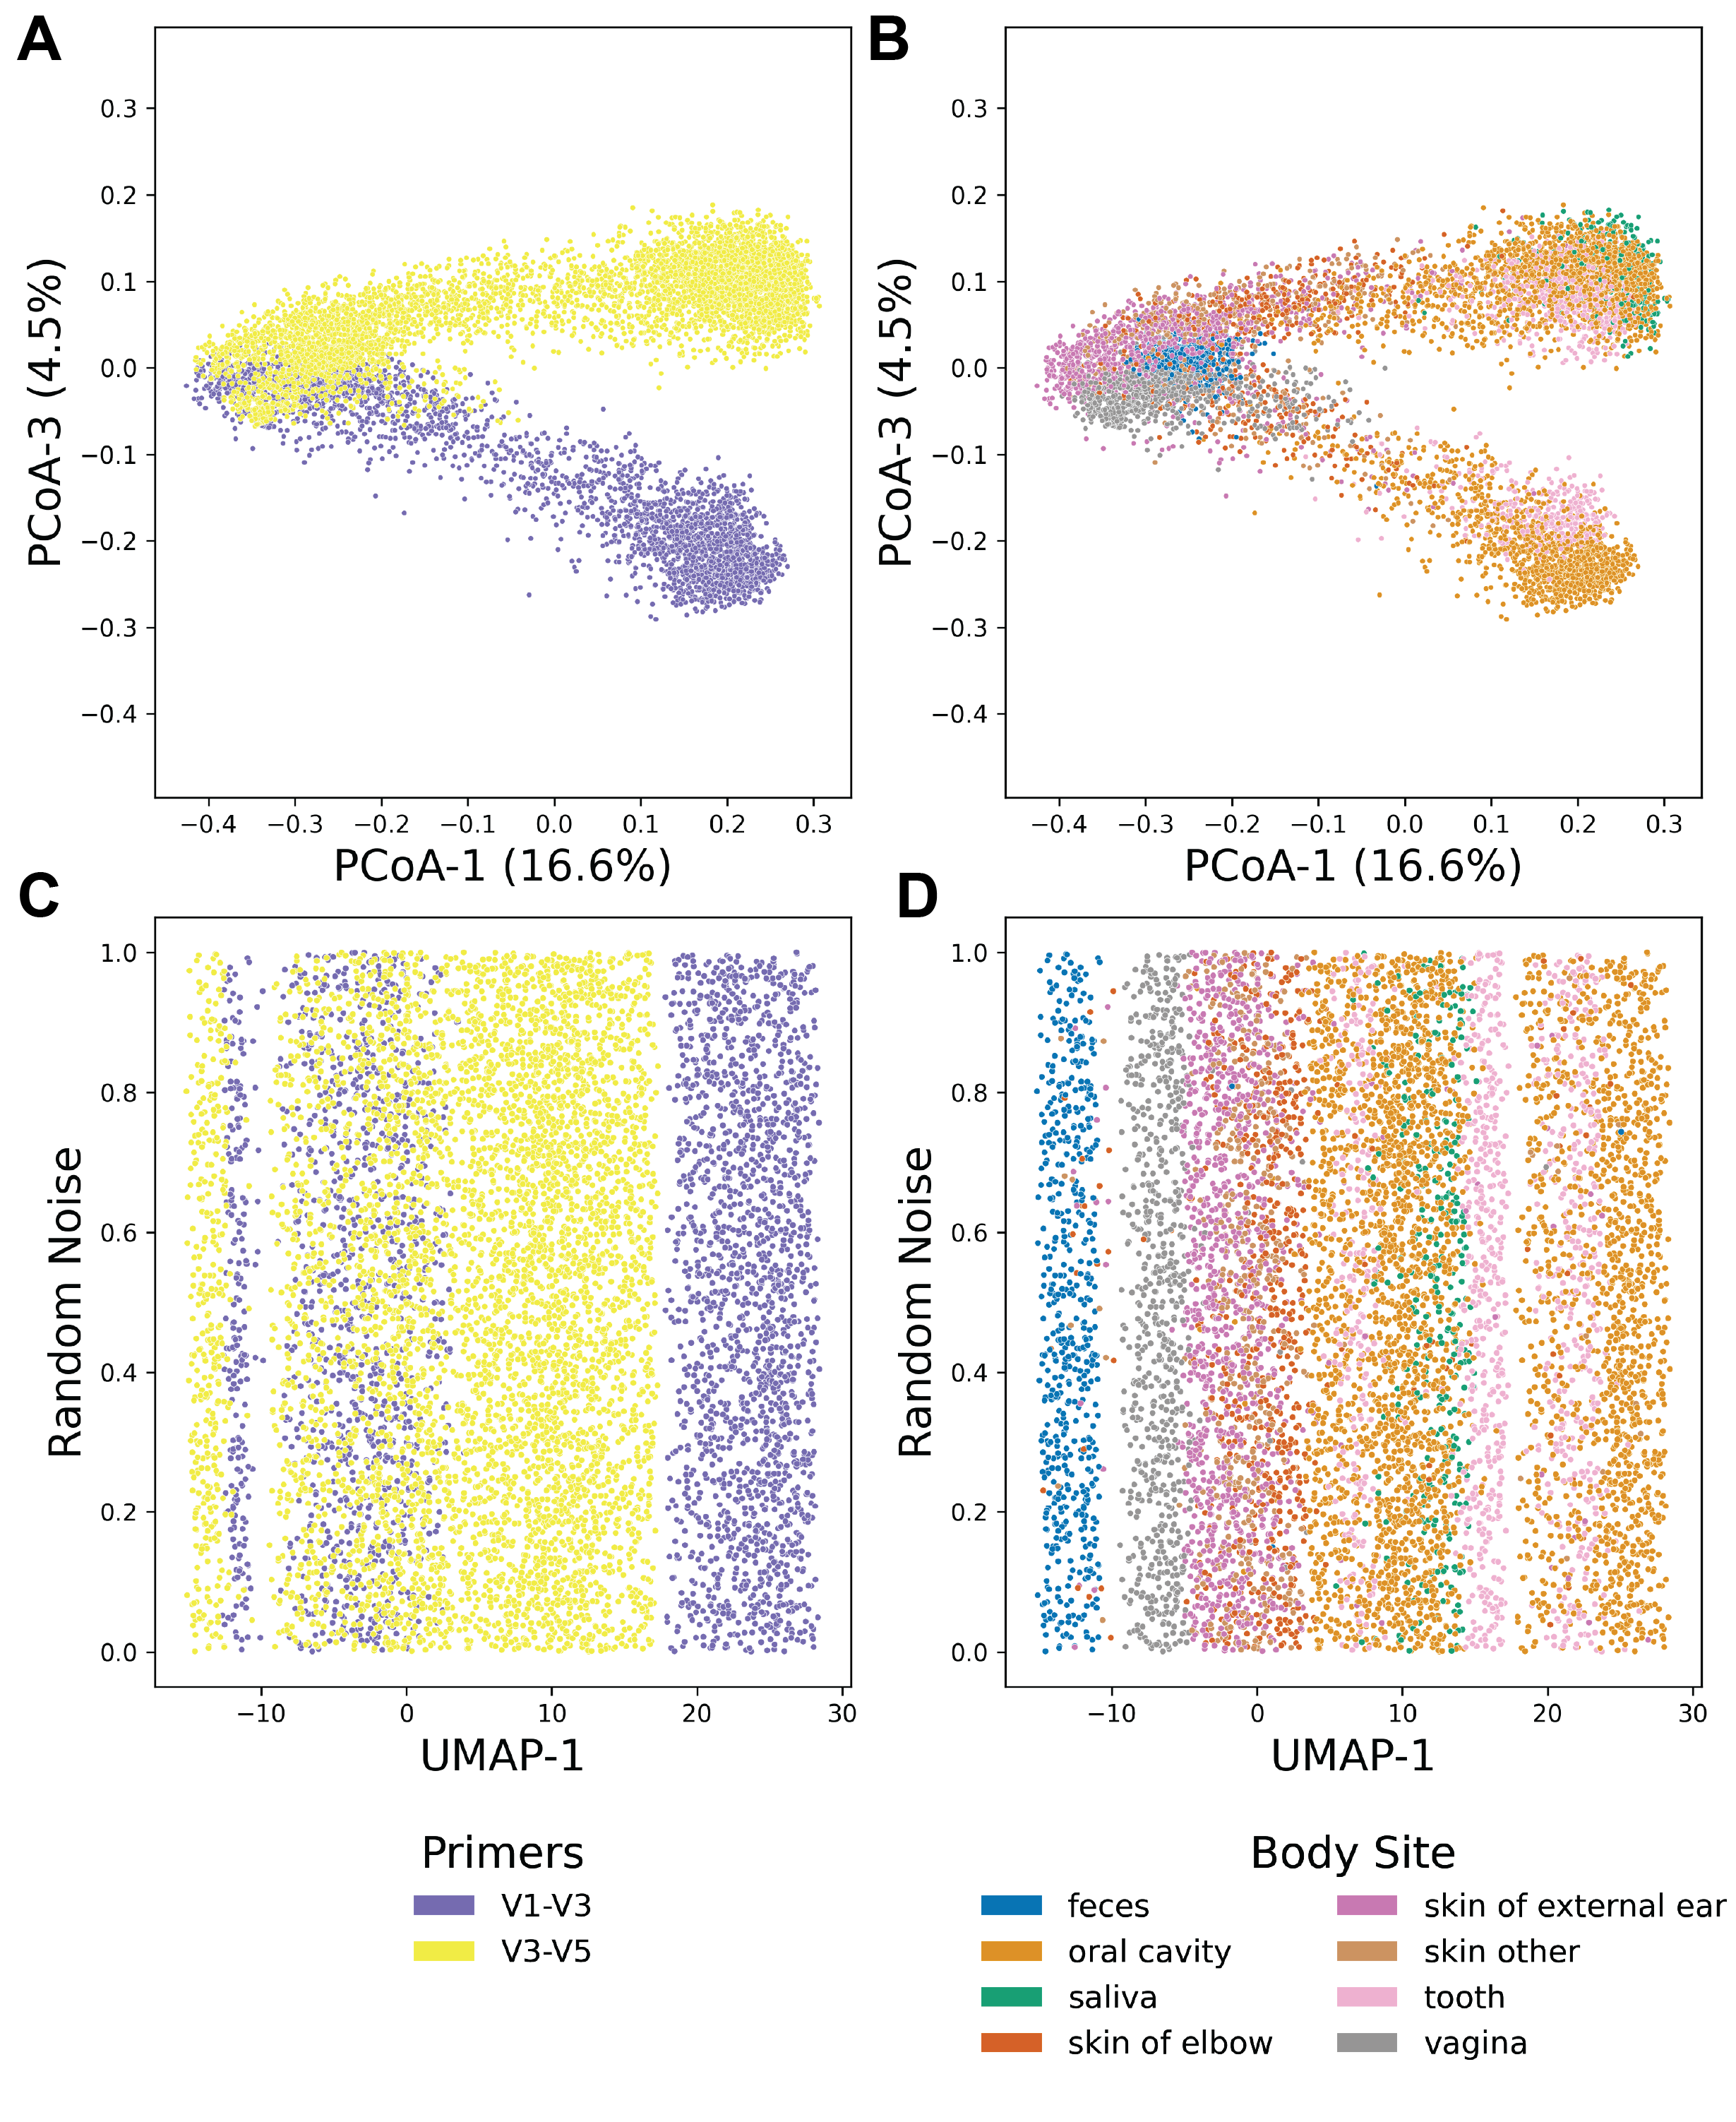
\includegraphics[width=\textwidth]{umap-figures/figureS03.png}
\caption[ Alternative views for PCoA and UMAP comparison on 8,280 samples from the Human Microbiome Project (HMP).]{\textbf{ Alternative views for PCoA and UMAP comparison on 8,280 samples from the Human Microbiome Project (HMP).} (A) PCoA-3 shows separation by primers and (B) some symmetry of sample site by primer. (C) UMAP separates the primers as well as (D) body sites in only one dimension.}
\label{umap_figS3}
\end{figure}


\chapter{Supplemental Material for Chapter~\ref{chapter_host_filtering}}

\begin{figure}[htbp]
\centering
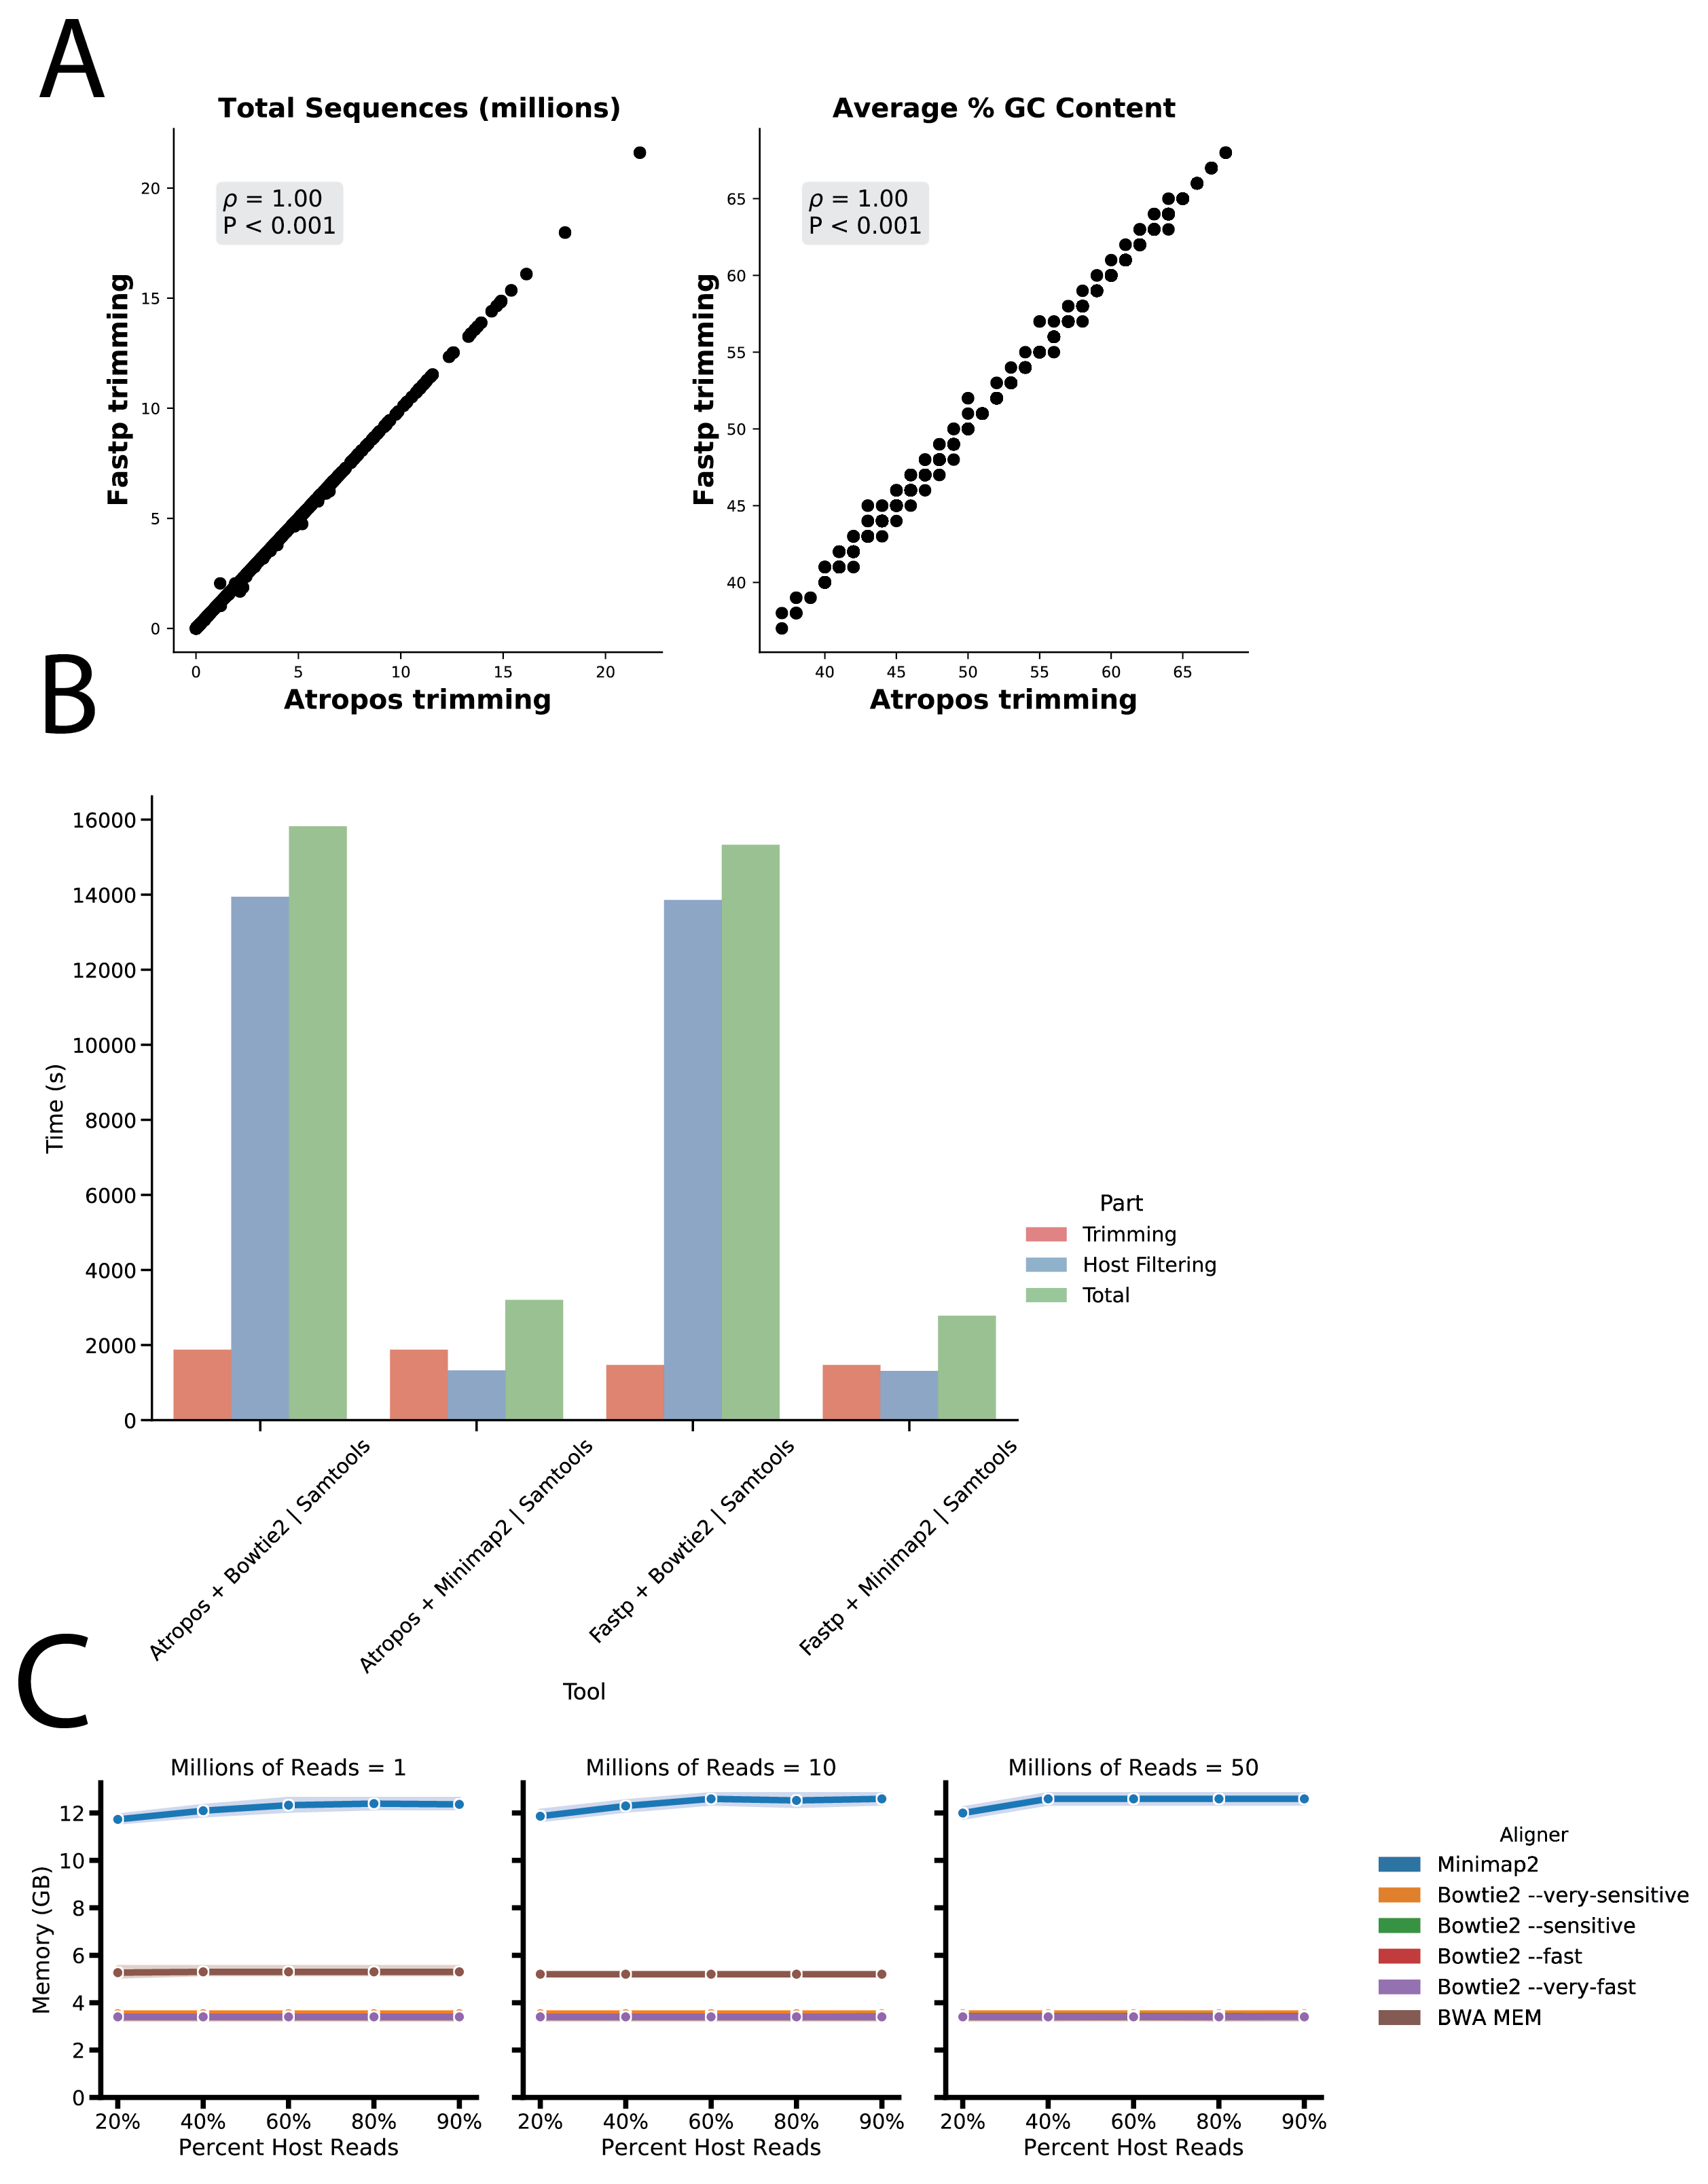
\includegraphics[width=0.9\textwidth]{host-filtering-figures/figureS01.png}
\caption[Comparison of total processing pipeline. ]{\textbf{Comparison of total processing pipeline. } (A) Comparison of trimming results on the kit extraction samples from reference 3. Each point represents the content of one sample. (B) Runtime (seconds) (y axis) between Fastp/Minimap2 and Atropos/Bowtie2 (x axis). (C) Peak memory usage for aligners using the CAMI-Sim simulated reads.}
\label{host_filtering_figS1}
\end{figure}

\begin{figure}[htbp]
\centering
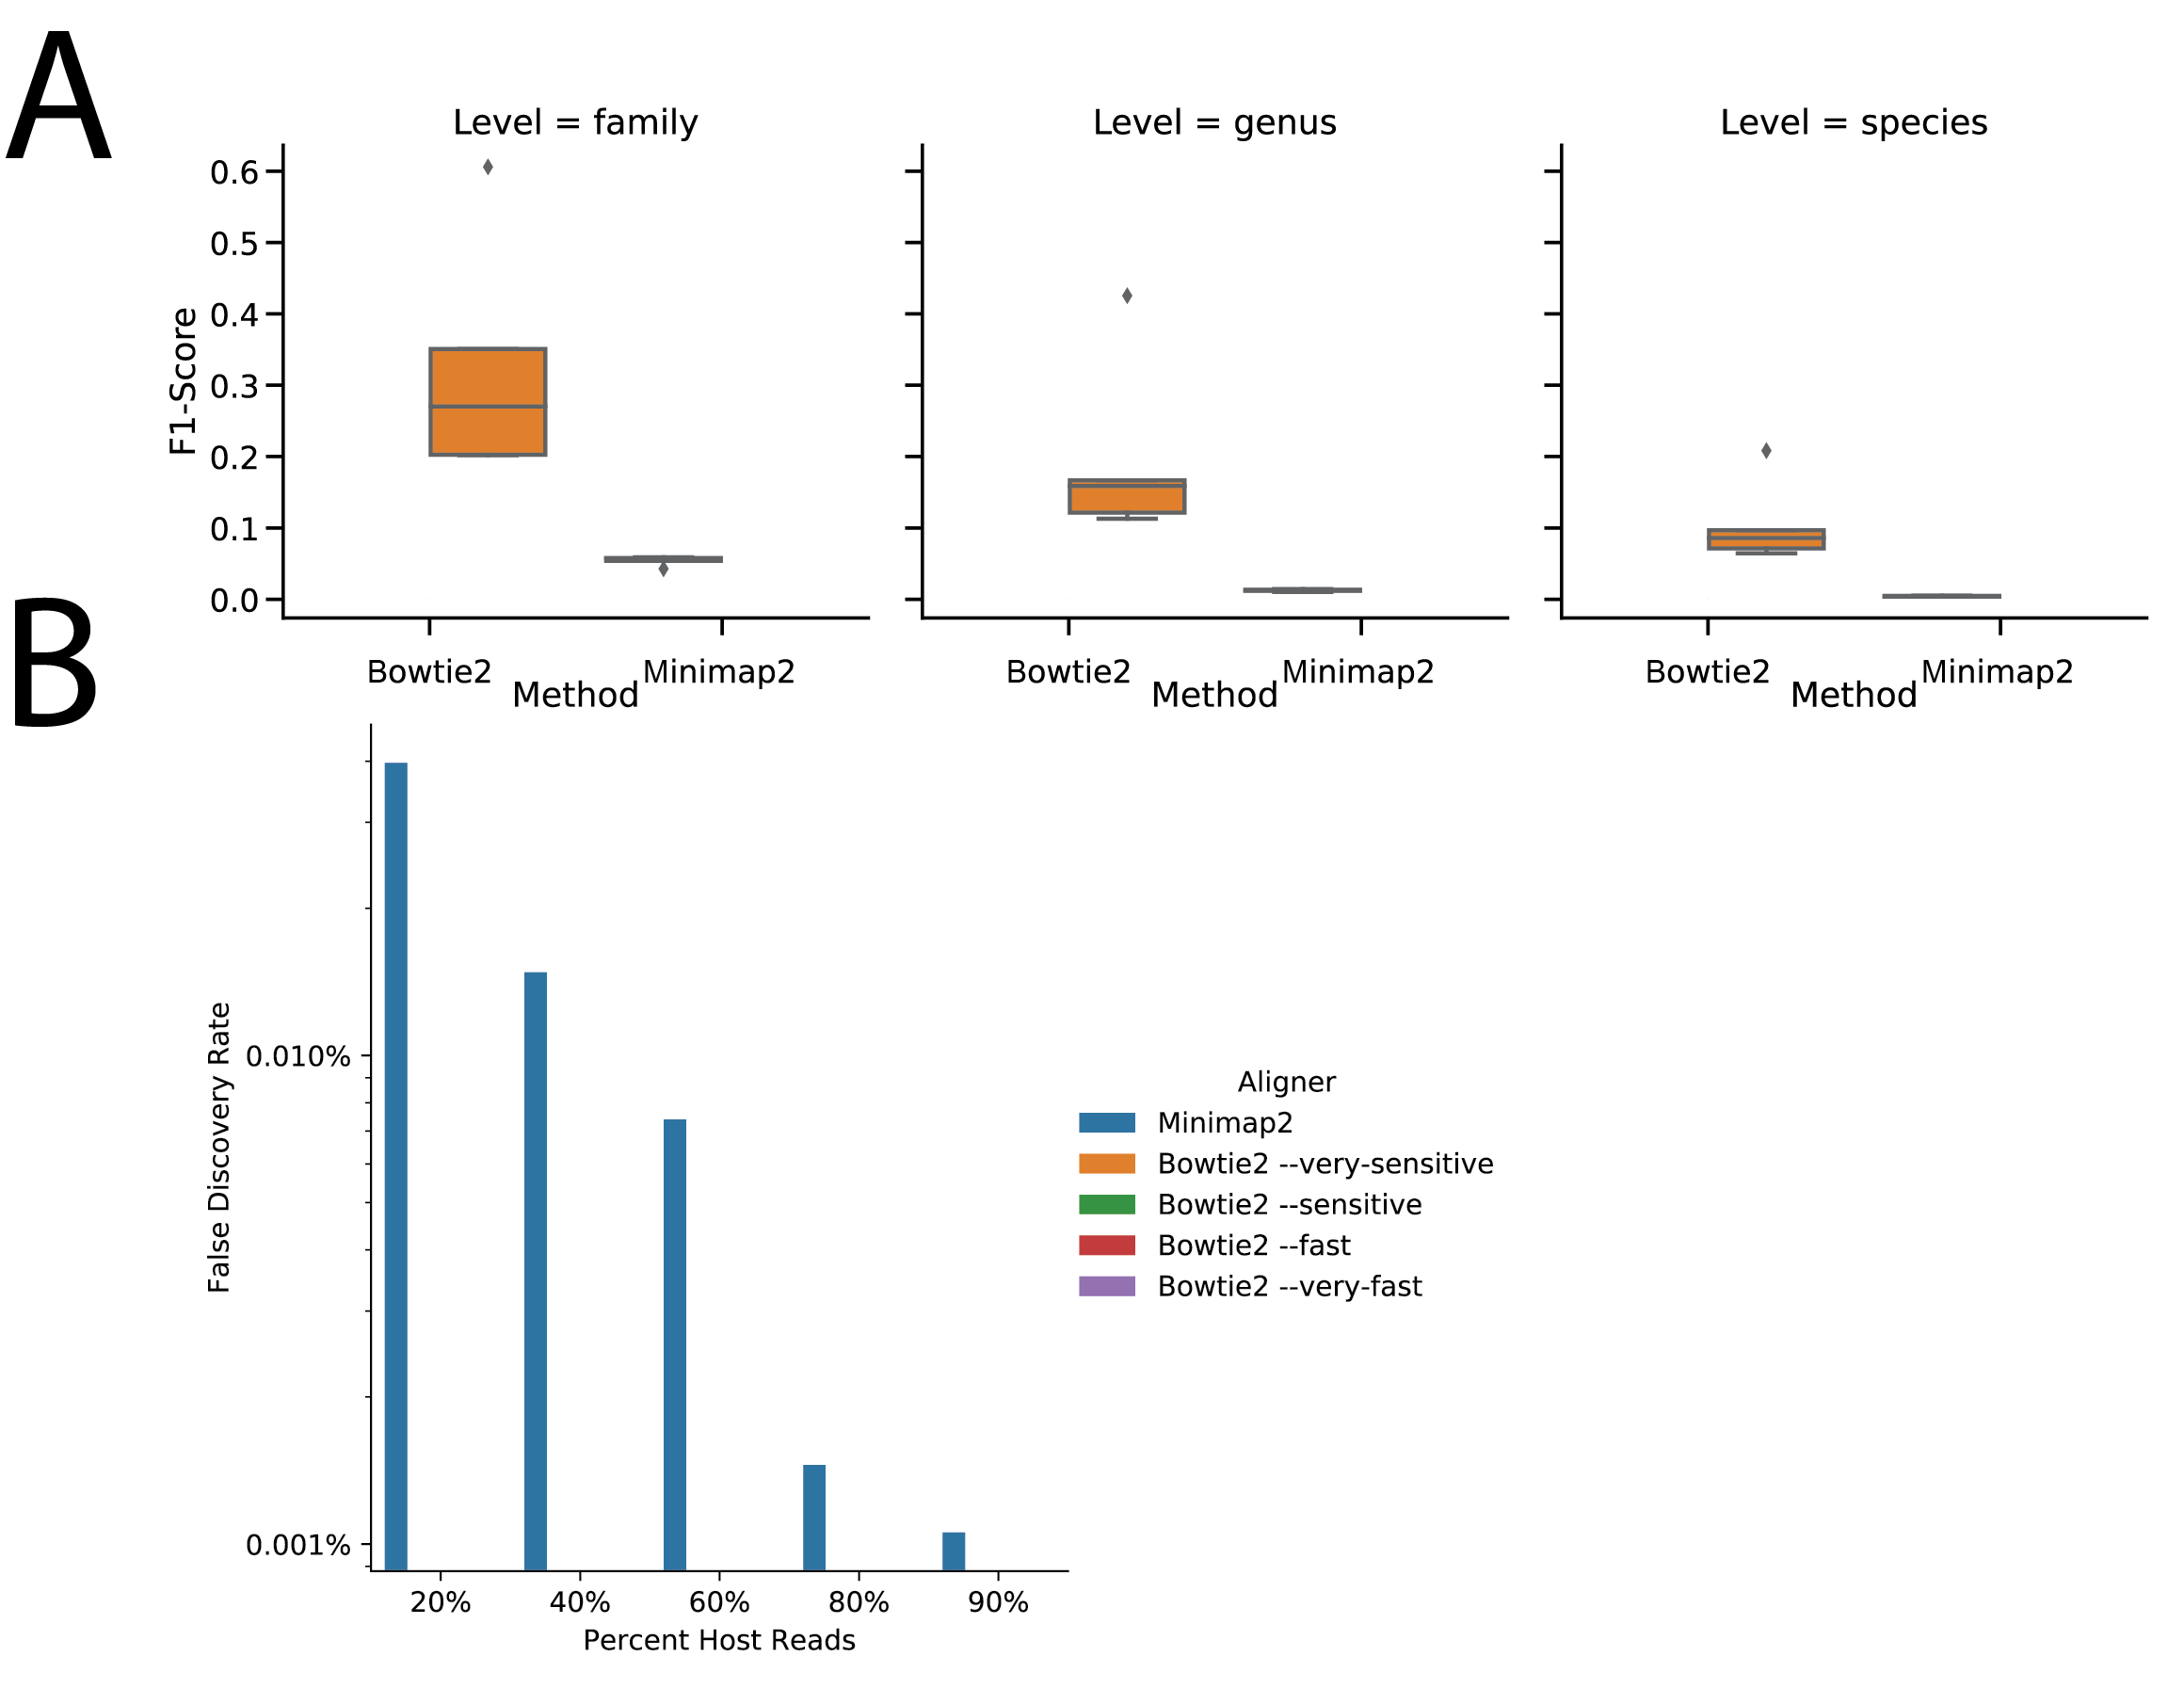
\includegraphics[width=\textwidth]{host-filtering-figures/figureS02.png}
\caption[Minimap2 gives poor taxonomic assignment compared to commonly used methods.]{\textbf{Minimap2 gives poor taxonomic assignment compared to commonly used methods.} (A) Comparison of Minimap2 and Bowtie2 (default) by F1 scores of taxon identification at family, genus, and species levels. (B) False discovery rate of Minimap2 and Bowtie2 for host filtering on the simulation data from Figure~\ref{host_filtering_fig1}A and B. Bars not shown indicate a value of 0.}
\label{host_filtering_figS2}
\end{figure}

\begin{table}

\caption[Refseq Assembly Accessions for Genomes included in simulation data]{Refseq Assembly Accessions for Genomes included in simulation data.}
\label{host_filtering_table_S1}

\centering
\begin{tabular}{ll} \hline
organism\_name          & refseq\_assembly\_accession  \\ 
\hline
\textit{Bacillus subtilis}       & GCF\_000009045.1             \\
\textit{Listeria monocytogenes}  & GCF\_000196035.1             \\
\textit{Staphylococcus aureus}   & GCF\_000013425.1             \\
\textit{Enterococcus faecalis}   & GCF\_000415185.1             \\
\textit{Lactobacillus fermentum} & GCF\_000010145.1             \\
\textit{Salmonella enterica}     & GCF\_000195995.1             \\
\textit{Escherichia coli }       & GCF\_000008865.2             \\
\textit{Pseudomonas aeruginosa } & GCF\_000006765.1             \\
\textit{Homo sapiens}          & GCF\_000001405.39           \\ \hline
\end{tabular}

\end{table}

\begin{table}
    \caption[ Exome sequencing data summary]{ Exome sequencing data summary.}
    \label{host_filtering_table_S2}
    \centering
    Table~\ref{host_filtering_table_S2} can be downloaded \href{https://journals.asm.org/doi/suppl/10.1128/msystems.01378-21/suppl_file/msystems.01378-21-st002.xlsx}{here}.
\end{table}


% \appendix
% \chapter{Supplemental Material for 
Chapter~\ref{chapter_umap}}

\begin{figure}[htbp]
\centering
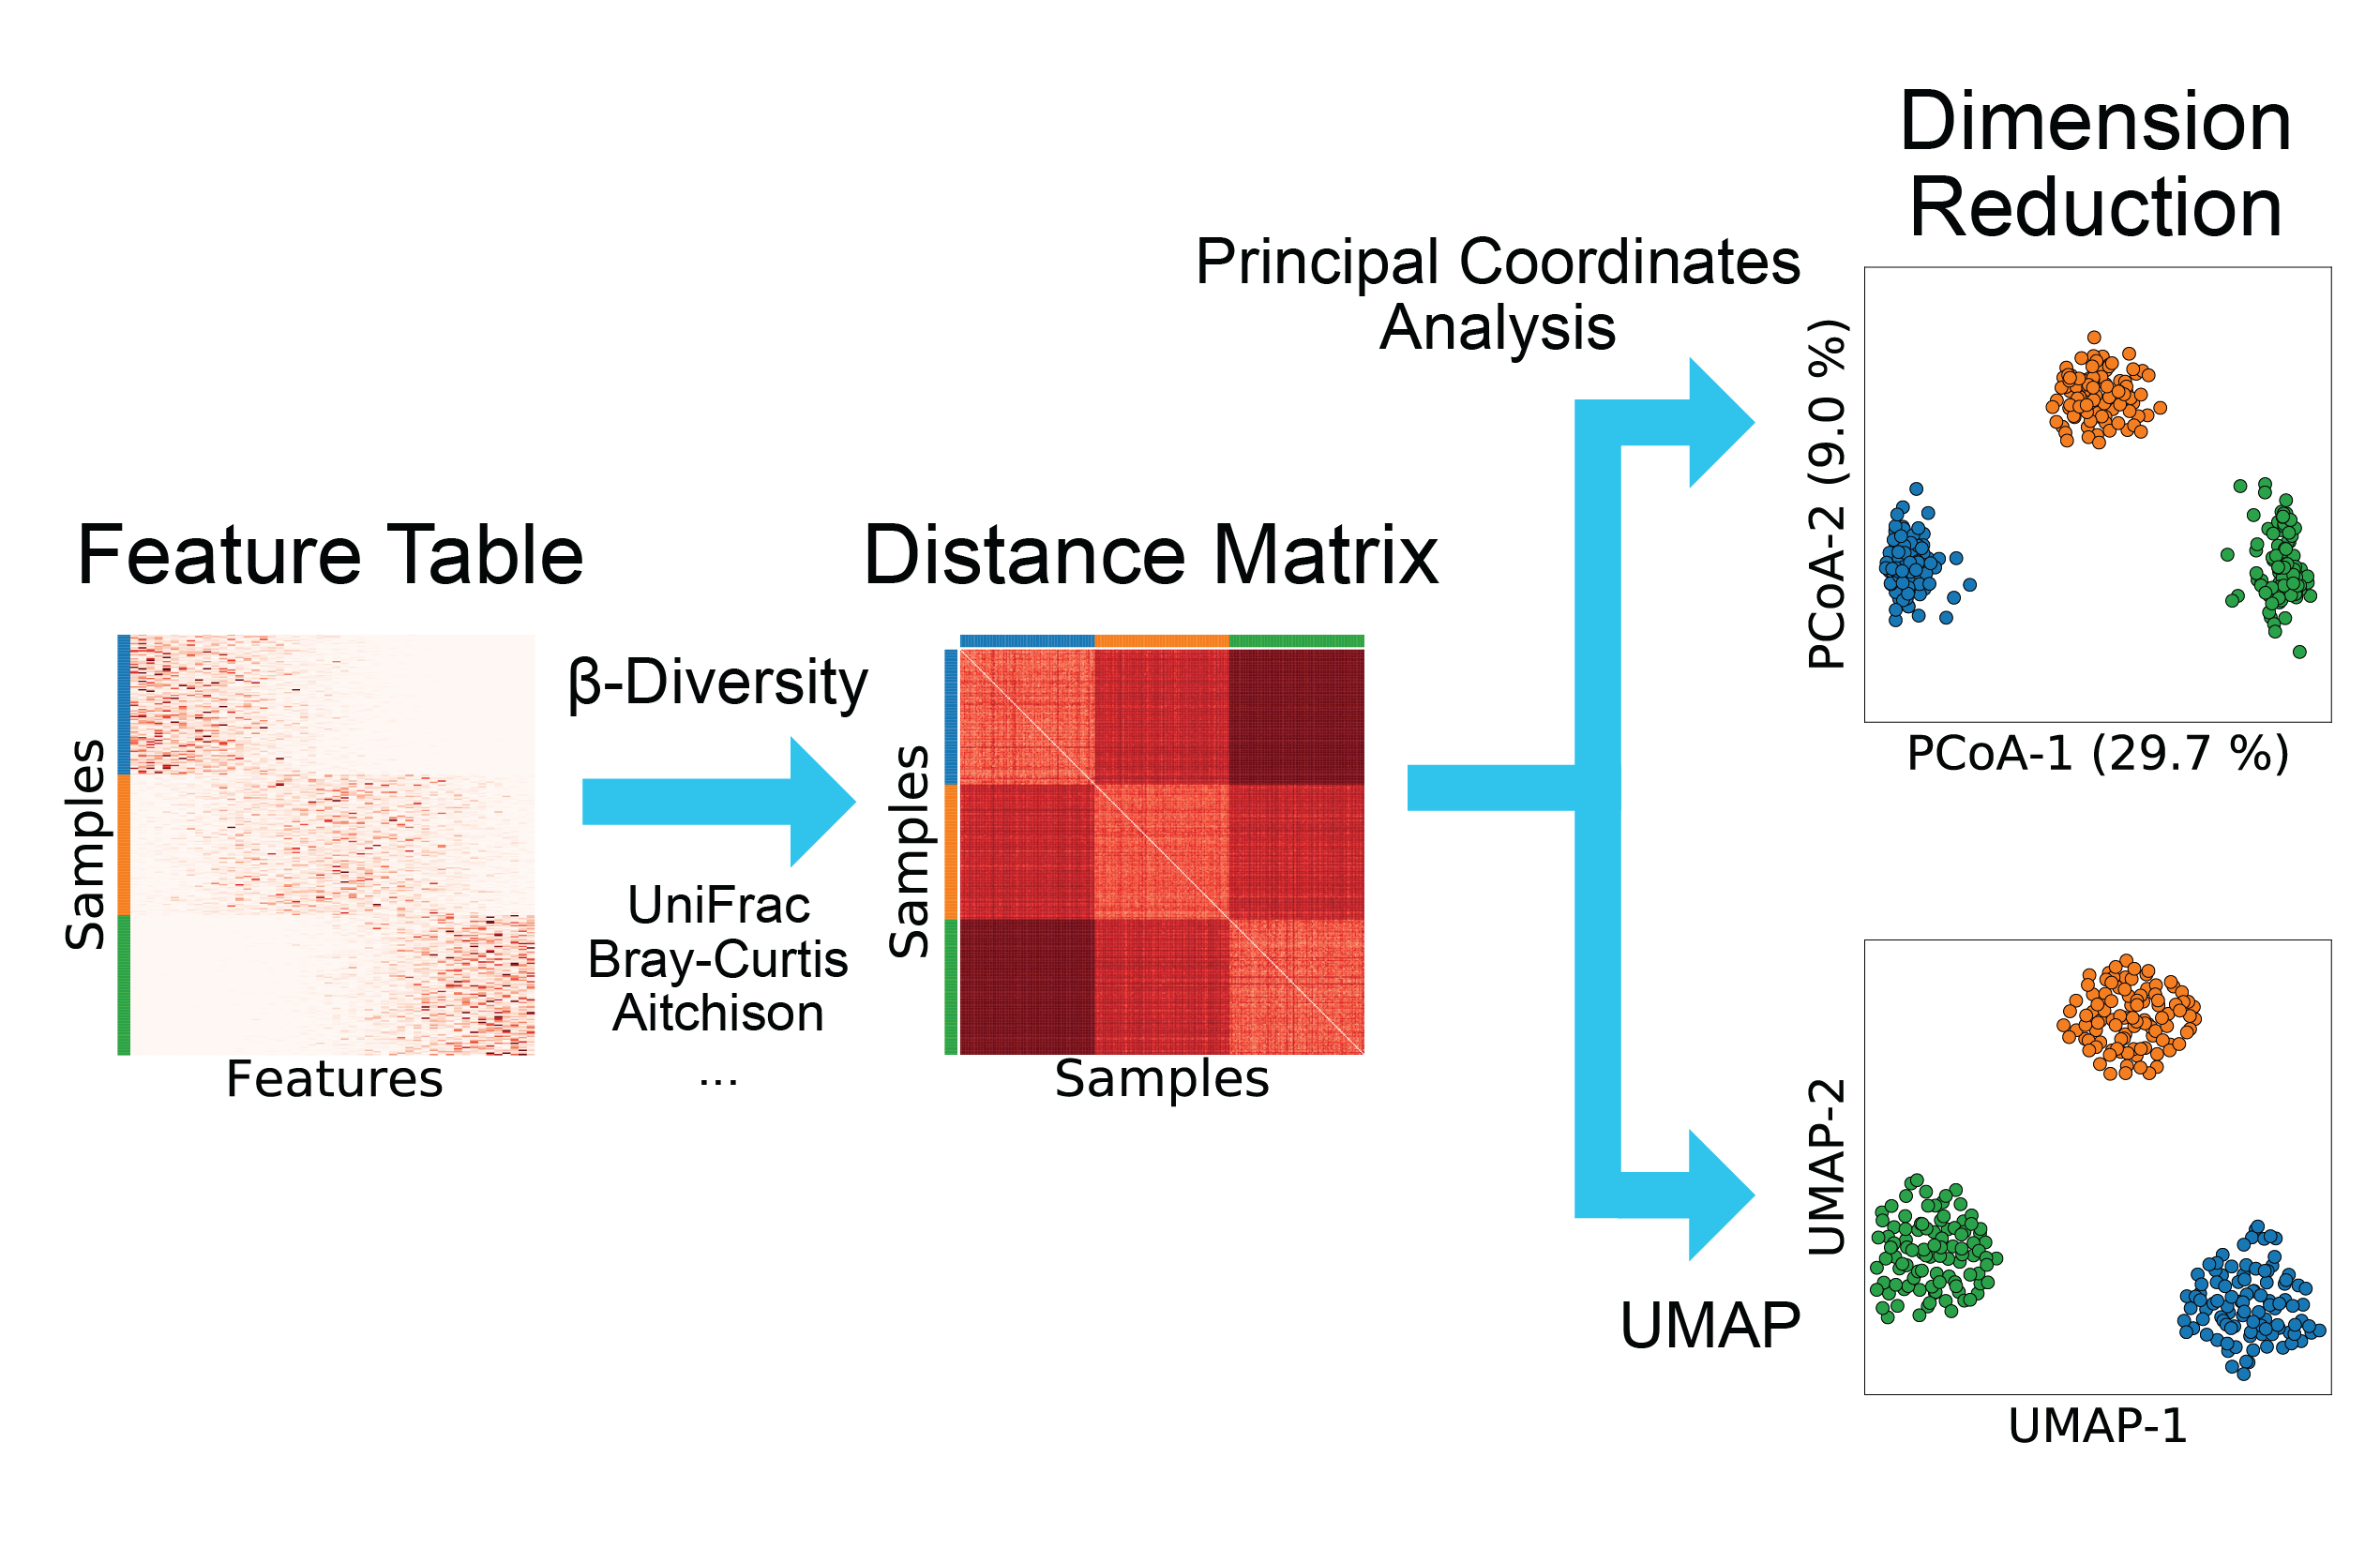
\includegraphics[width=\textwidth]{umap-figures/figureS01.png}
\caption[Graphical abstract.]{\textbf{Graphical abstract.} UMAP can operate on distance matrices of arbitrary distance metrics (UniFrac, Bray-Curtis, Aitchison), similarly to PCoA.}
\label{umap_figS1}
\end{figure}

\begin{figure}[htbp]
\centering
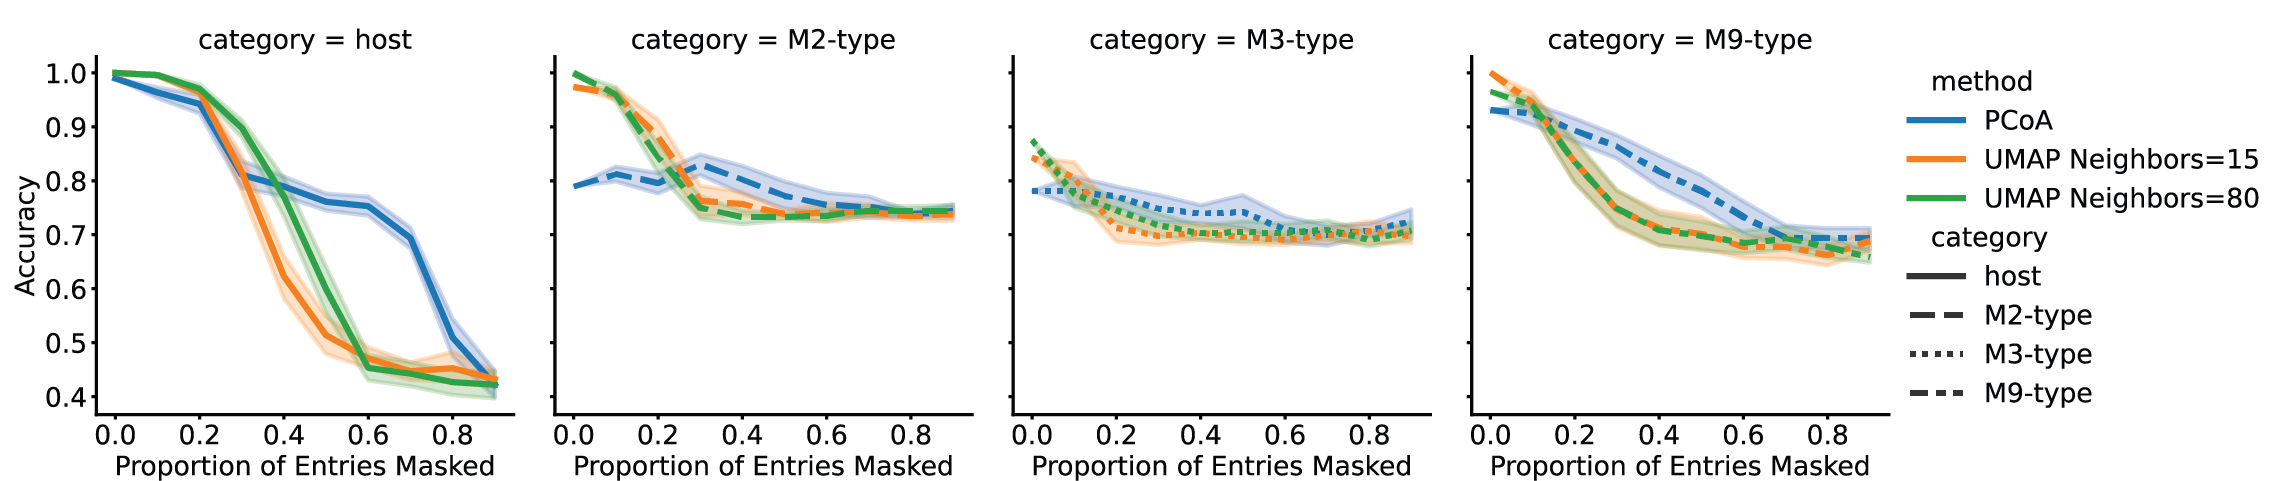
\includegraphics[width=\textwidth]{umap-figures/figureS02.png}
\caption[Simulated missing data on keyboard study.]{\textbf{Simulated missing data on keyboard study.} A proportion of the entries of the table were randomly masked (20 repetitions per ablation level) from the feature table, and dimensionality reduction followed by LDA was run on each of the tables. Host accuracy is the accuracy for identifying the correct subject. The subject-type accuracies are specific sample-type accuracies specific to the individual.}
\label{umap_figS2}
\end{figure}

\begin{figure}[htbp]
\centering
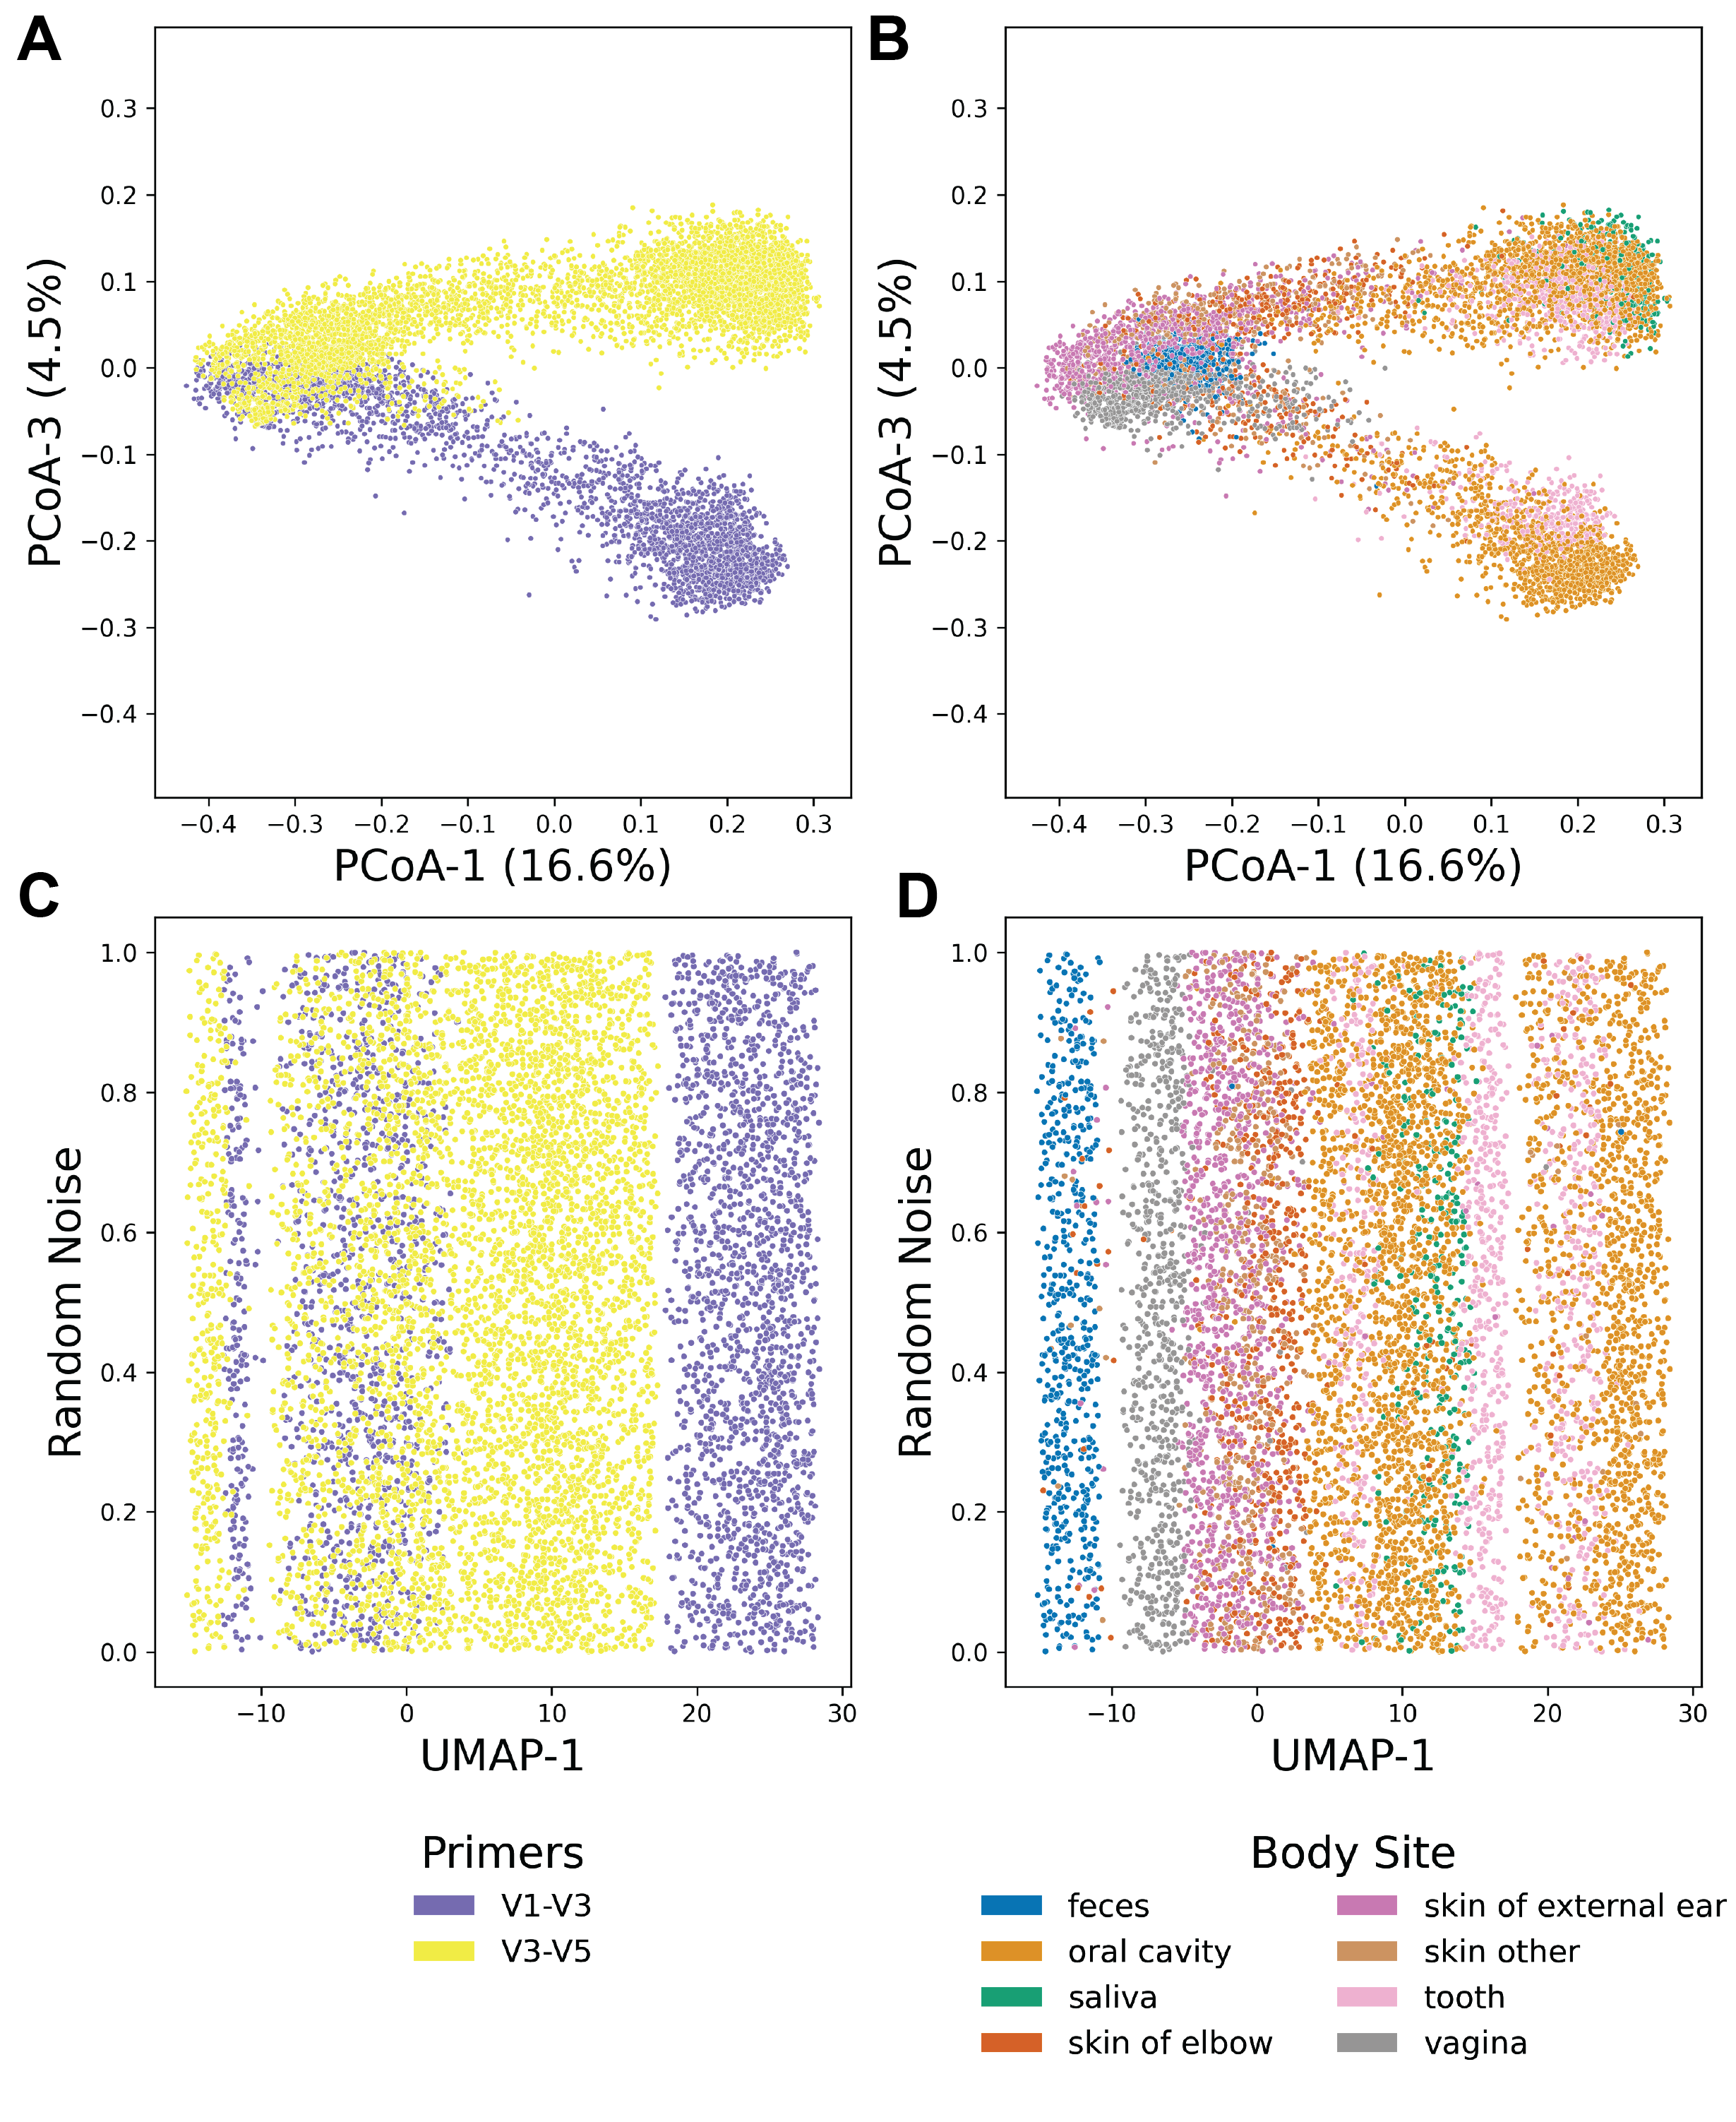
\includegraphics[width=\textwidth]{umap-figures/figureS03.png}
\caption[ Alternative views for PCoA and UMAP comparison on 8,280 samples from the Human Microbiome Project (HMP).]{\textbf{ Alternative views for PCoA and UMAP comparison on 8,280 samples from the Human Microbiome Project (HMP).} (A) PCoA-3 shows separation by primers and (B) some symmetry of sample site by primer. (C) UMAP separates the primers as well as (D) body sites in only one dimension.}
\label{umap_figS3}
\end{figure}


\chapter{Supplemental Material for Chapter~\ref{chapter_host_filtering}}

\begin{figure}[htbp]
\centering
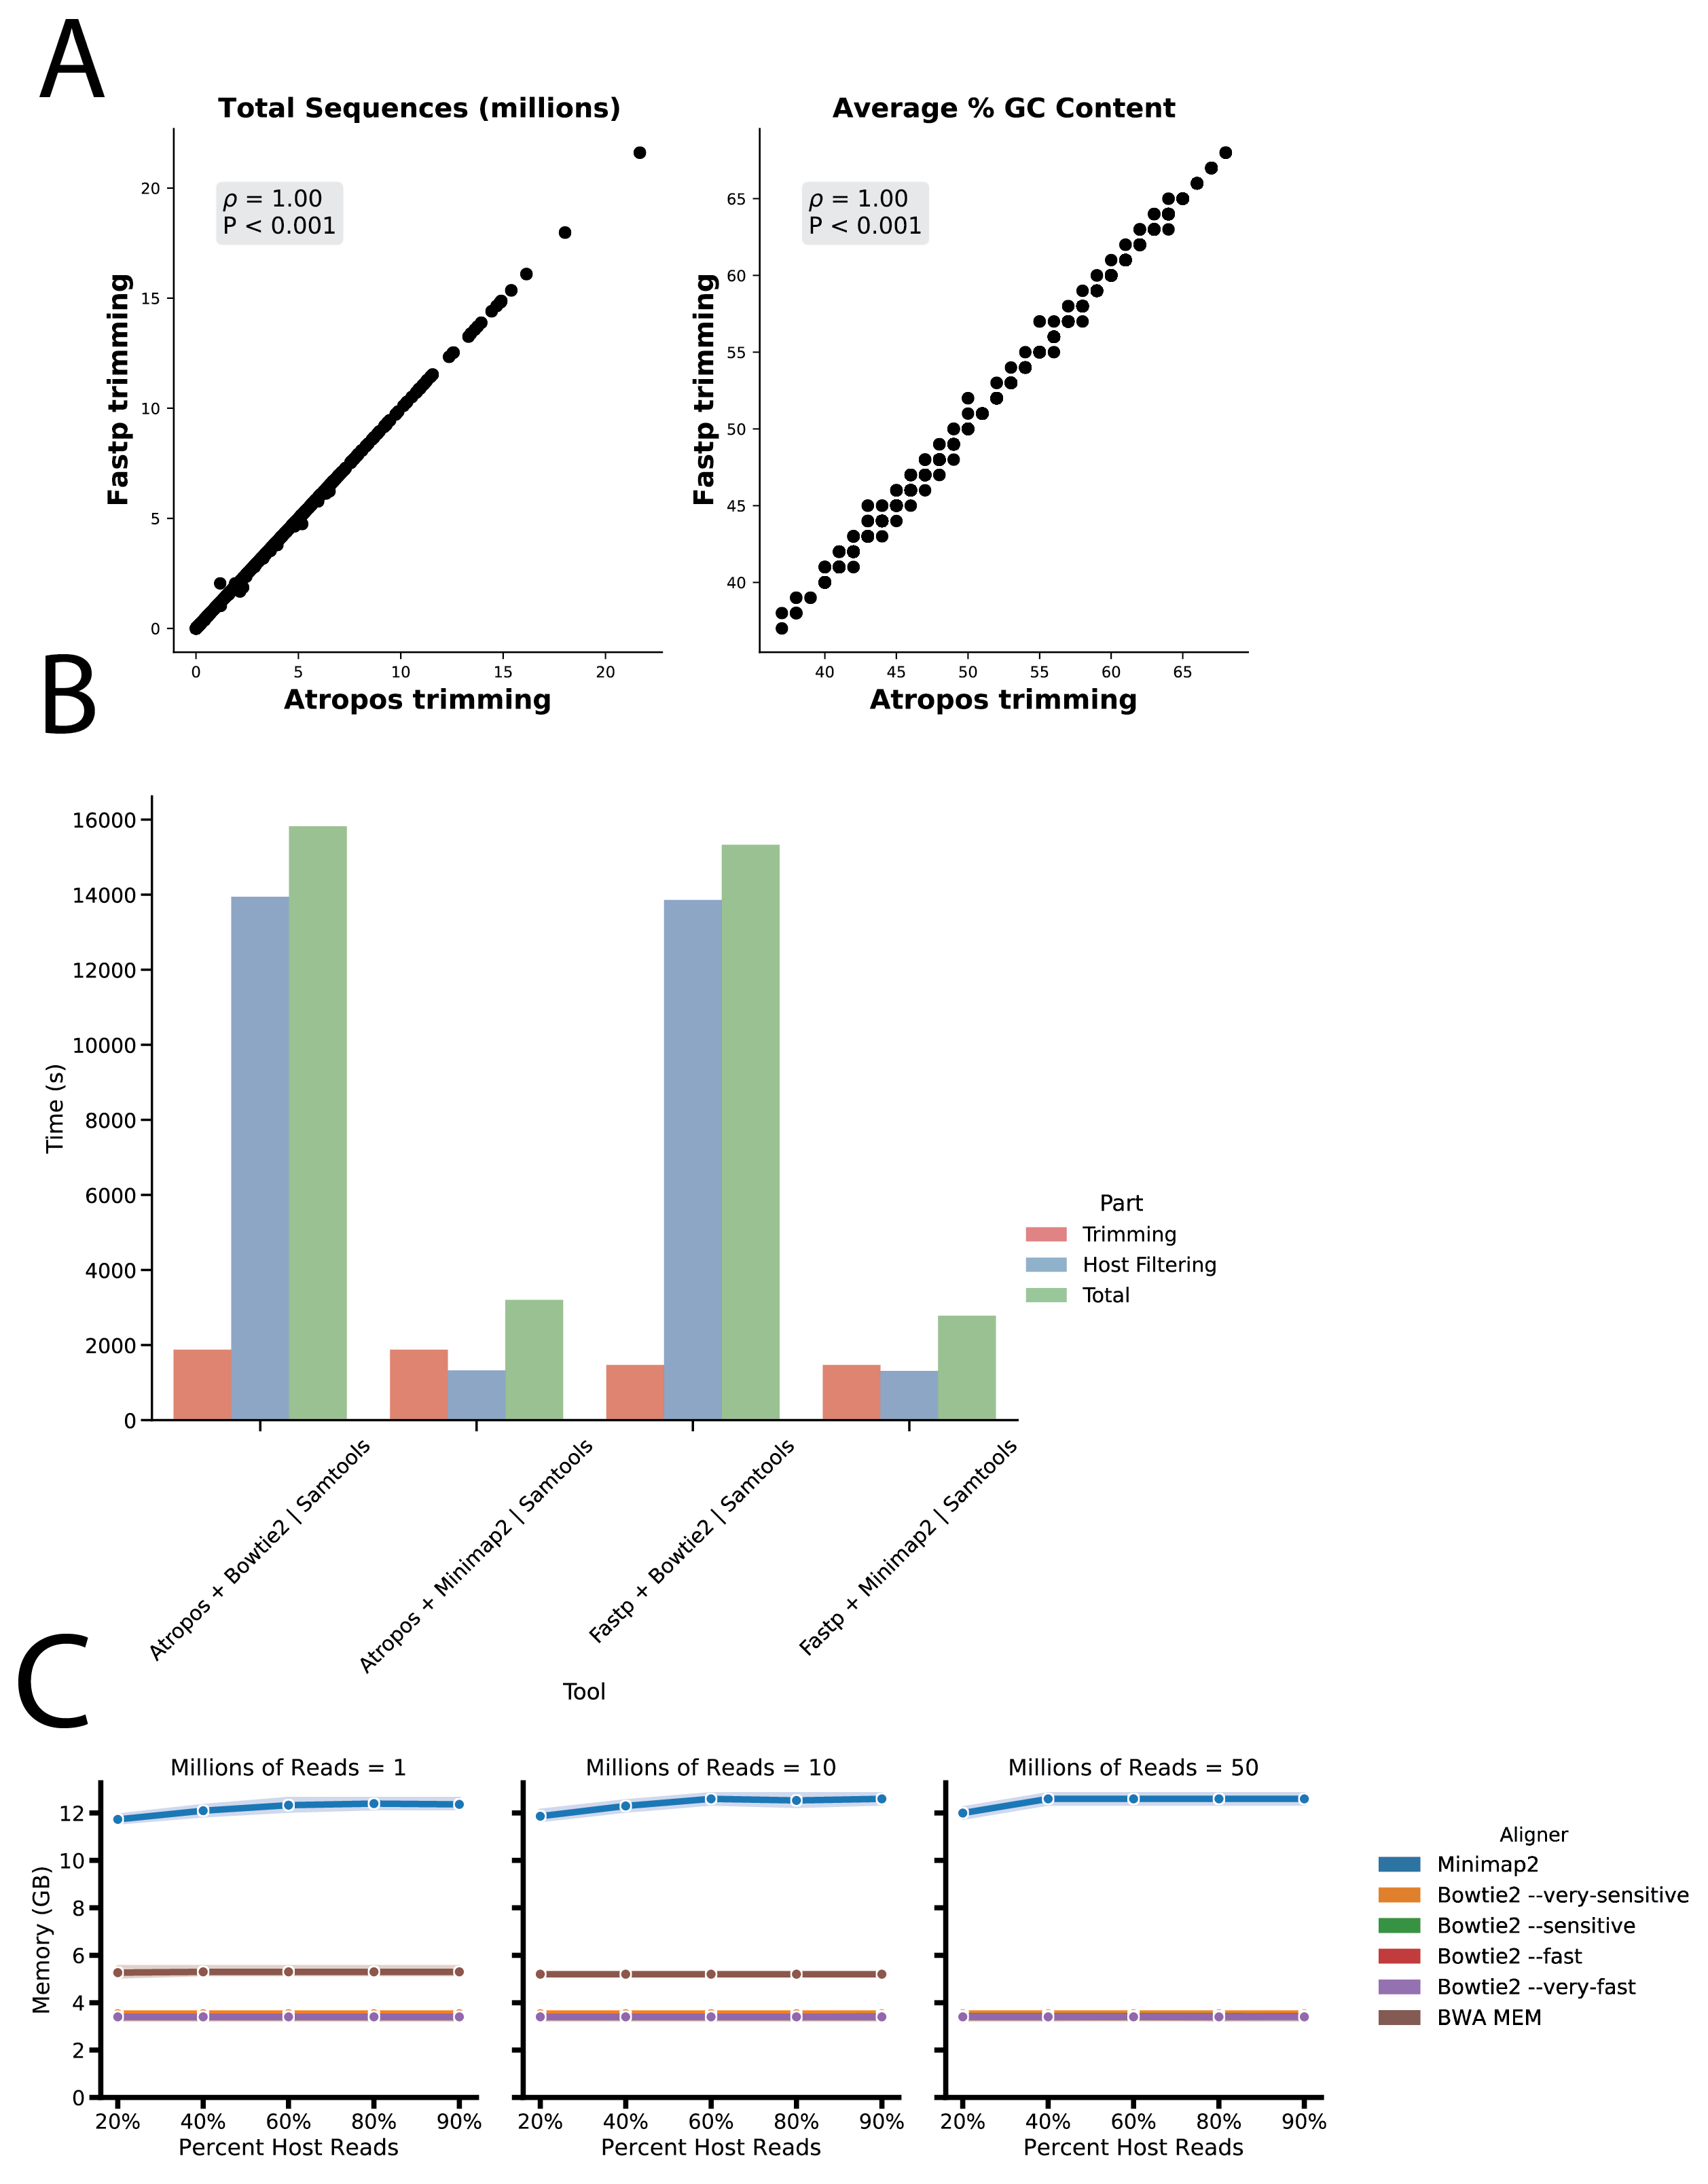
\includegraphics[width=0.9\textwidth]{host-filtering-figures/figureS01.png}
\caption[Comparison of total processing pipeline. ]{\textbf{Comparison of total processing pipeline. } (A) Comparison of trimming results on the kit extraction samples from reference 3. Each point represents the content of one sample. (B) Runtime (seconds) (y axis) between Fastp/Minimap2 and Atropos/Bowtie2 (x axis). (C) Peak memory usage for aligners using the CAMI-Sim simulated reads.}
\label{host_filtering_figS1}
\end{figure}

\begin{figure}[htbp]
\centering
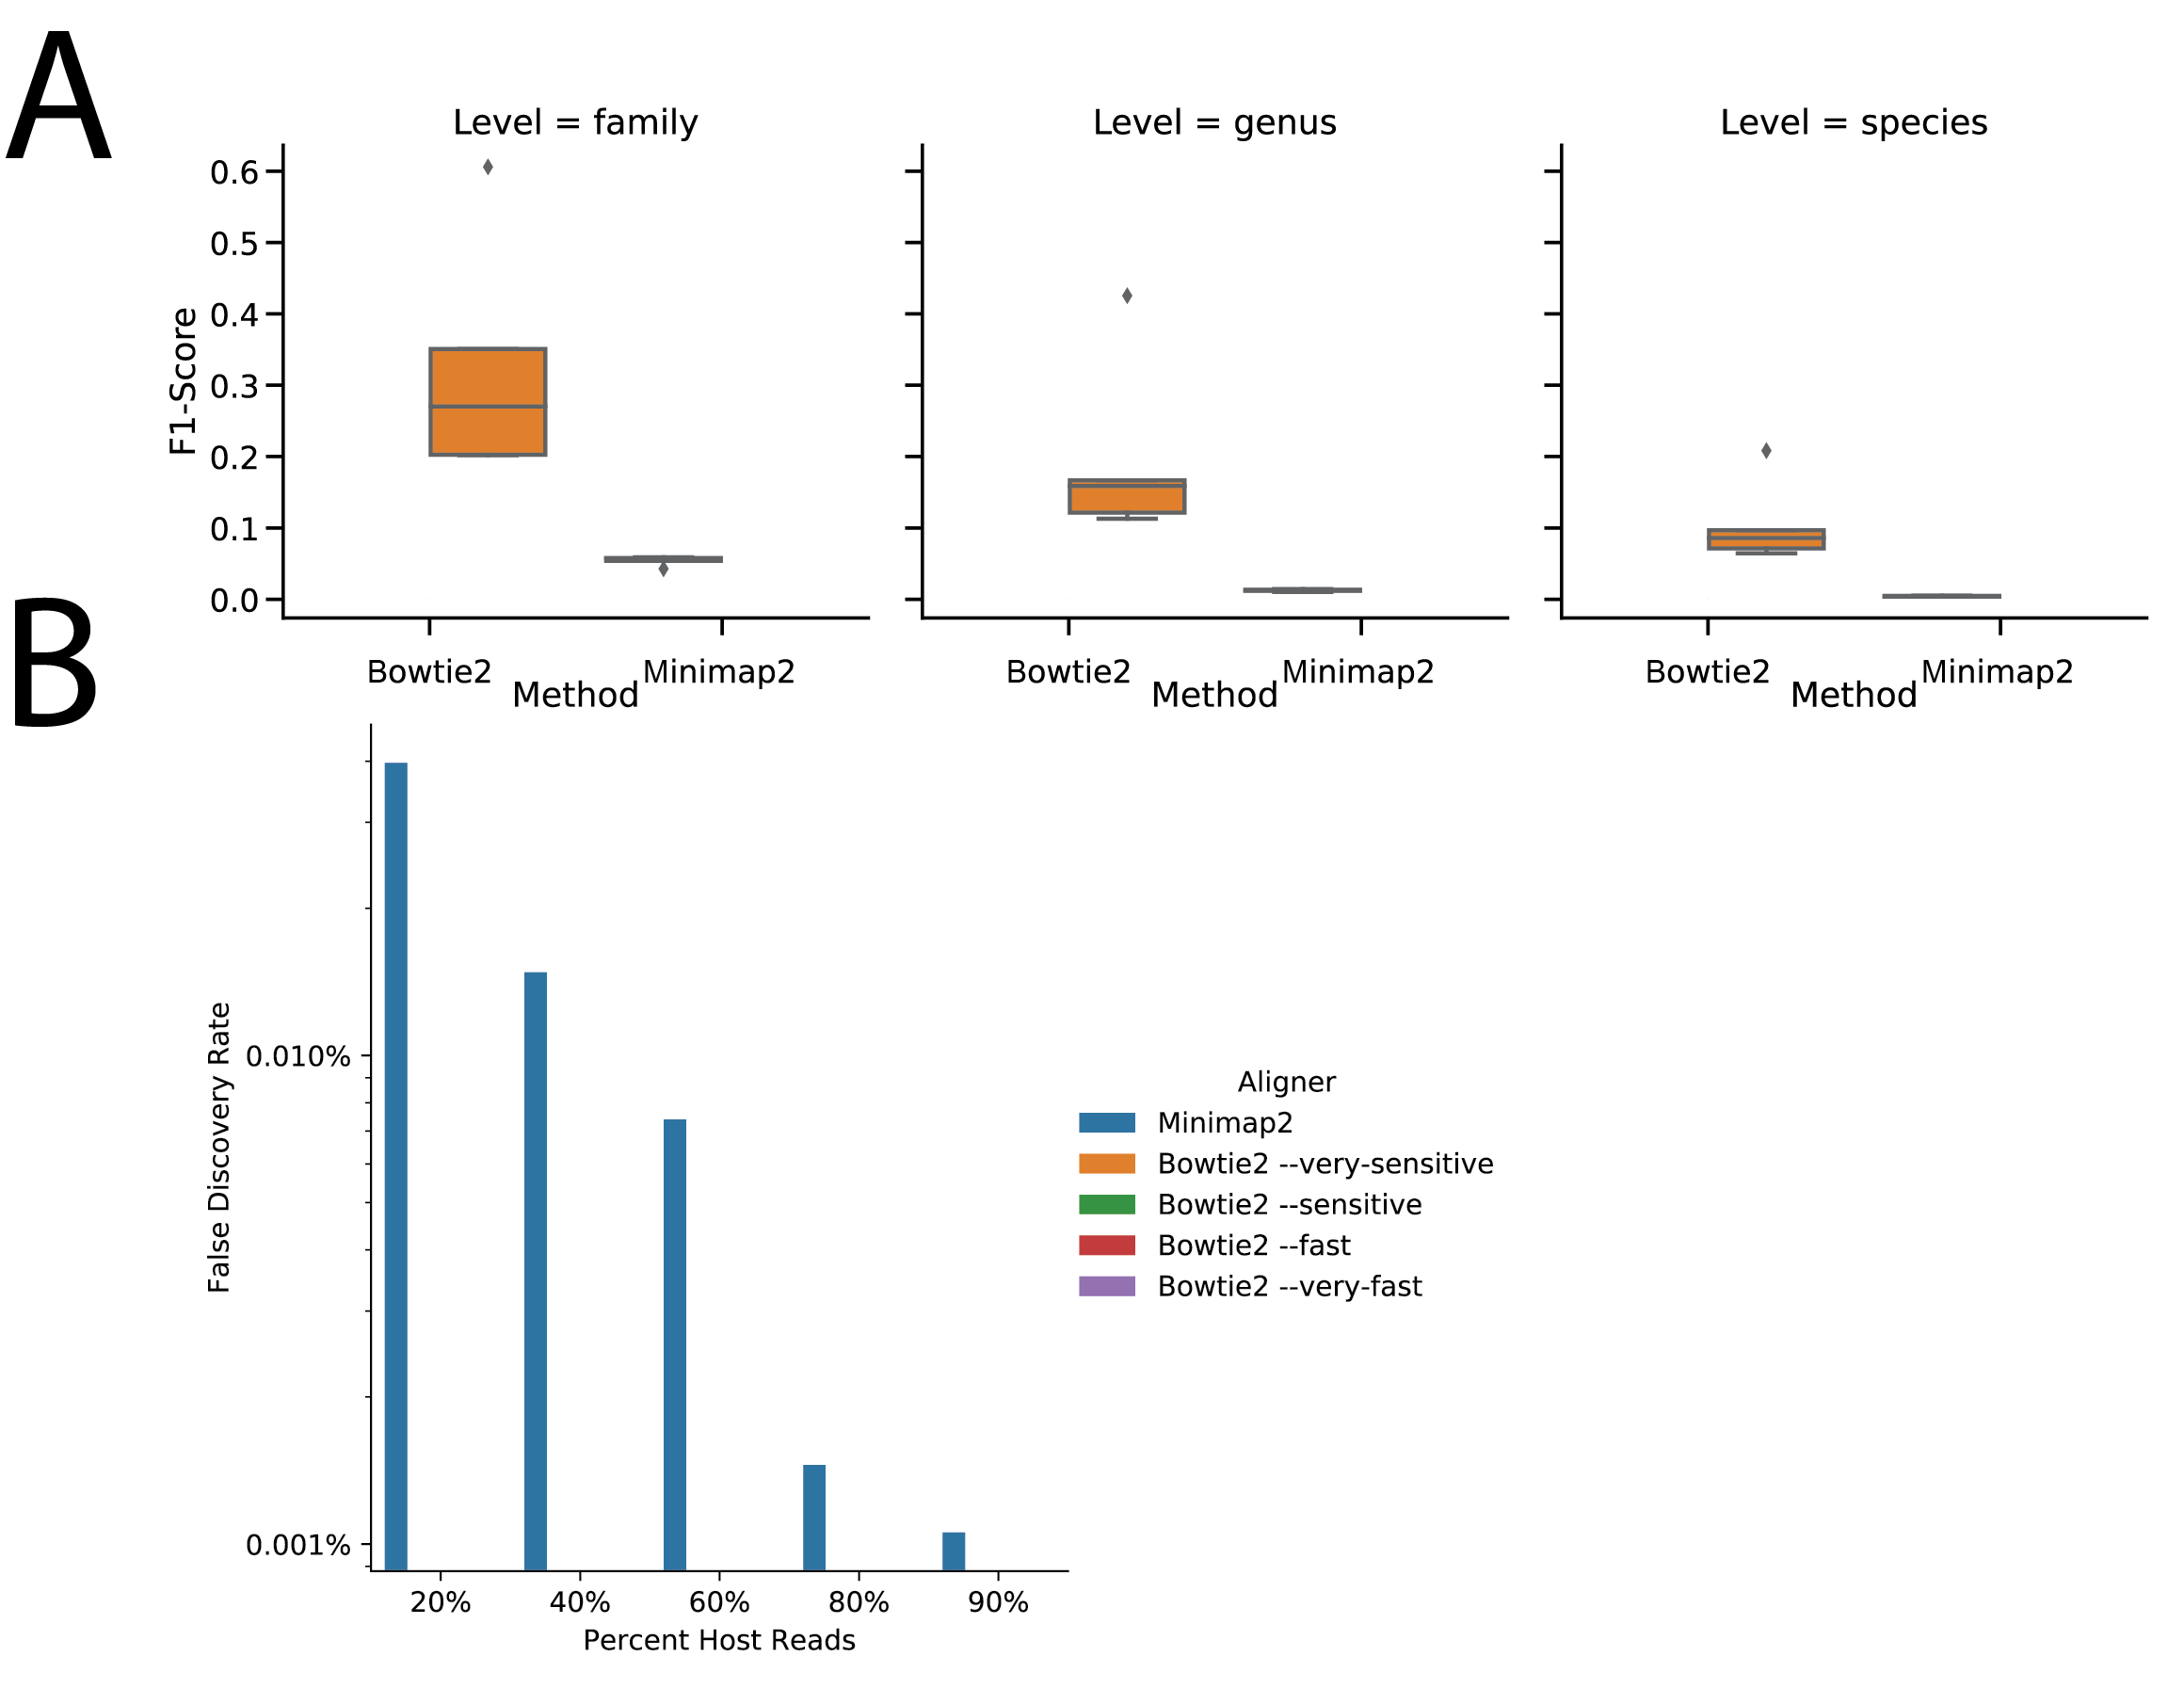
\includegraphics[width=\textwidth]{host-filtering-figures/figureS02.png}
\caption[Minimap2 gives poor taxonomic assignment compared to commonly used methods.]{\textbf{Minimap2 gives poor taxonomic assignment compared to commonly used methods.} (A) Comparison of Minimap2 and Bowtie2 (default) by F1 scores of taxon identification at family, genus, and species levels. (B) False discovery rate of Minimap2 and Bowtie2 for host filtering on the simulation data from Figure~\ref{host_filtering_fig1}A and B. Bars not shown indicate a value of 0.}
\label{host_filtering_figS2}
\end{figure}

\begin{table}

\caption[Refseq Assembly Accessions for Genomes included in simulation data]{Refseq Assembly Accessions for Genomes included in simulation data.}
\label{host_filtering_table_S1}

\centering
\begin{tabular}{ll} \hline
organism\_name          & refseq\_assembly\_accession  \\ 
\hline
\textit{Bacillus subtilis}       & GCF\_000009045.1             \\
\textit{Listeria monocytogenes}  & GCF\_000196035.1             \\
\textit{Staphylococcus aureus}   & GCF\_000013425.1             \\
\textit{Enterococcus faecalis}   & GCF\_000415185.1             \\
\textit{Lactobacillus fermentum} & GCF\_000010145.1             \\
\textit{Salmonella enterica}     & GCF\_000195995.1             \\
\textit{Escherichia coli }       & GCF\_000008865.2             \\
\textit{Pseudomonas aeruginosa } & GCF\_000006765.1             \\
\textit{Homo sapiens}          & GCF\_000001405.39           \\ \hline
\end{tabular}

\end{table}

\begin{table}
    \caption[ Exome sequencing data summary]{ Exome sequencing data summary.}
    \label{host_filtering_table_S2}
    \centering
    Table~\ref{host_filtering_table_S2} can be downloaded \href{https://journals.asm.org/doi/suppl/10.1128/msystems.01378-21/suppl_file/msystems.01378-21-st002.xlsx}{here}.
\end{table}


%% END MATTER
\printindex %% Uncomment to display the index
% \nocite{}  %% Put any references that you want to include in the bib 
%               but haven't cited in the braces.
% \bibliographystyle{alpha}  %% This is just my personal favorite style. 
%                              There are many others.
\bibliography{references}
\bibliographystyle{plain}

\end{document}
